%
%  Lectures on black holes at IAP
%
%%%%%%%%%%%%%%%%%%%%%%%%%%%%%%%%%%%%%%%%%%%%%%%%%%%%%%%%%%%%%%%%%%%%%%%%%%%%

\documentclass[12pt,a4paper]{book}
\usepackage[utf8]{inputenc}
\usepackage[T1]{fontenc}
\usepackage{hyperref}
\usepackage{makeidx} % generation de l'index
\usepackage[nottoc]{tocbibind} % bibliographie et index dans la table des matières
\usepackage{fancyhdr}
\usepackage{minitoc}
\usepackage{graphicx}
\usepackage{color}
\usepackage{bm} % bold math
\usepackage{amsmath}
\usepackage{amssymb} % symboles AMS (-> \mathbb)
\usepackage{amsthm}  % theorem-like environments
\usepackage{mathrsfs} % -> \mathscr

%%%%%%%%%%%%%%%%%%%%%%%%%%%%%%%%%%%%%%%%%%%%%%%%%%%%%%%%%%%%%%%%%%%%%%%%%%%%

% Reglages:
%
\hypersetup{pdftitle={Lectures on black holes},
  pdfsubject={black holes},
  pdfauthor={Eric Gourgoulhon <eric.gourgoulhon@obspm.fr>},
  pdfkeywords={LaTeX},
  colorlinks=true
}
\pagestyle{fancyplain}
\addtolength{\headwidth}{\marginparsep}
\addtolength{\headwidth}{\marginparwidth}
\renewcommand{\chaptermark}[1]{\markboth{#1}{}}
\renewcommand{\sectionmark}[1]{\markright{\thesection\ #1}}
\lhead[\fancyplain{}{\bfseries\thepage}]{}
\rhead[]{\fancyplain{}{\bfseries\thepage}}
\chead[\fancyplain{}{\bfseries\leftmark}]{\fancyplain{}{\bfseries\rightmark}}
\cfoot{}
%
\setcounter{minitocdepth}{1}
\renewcommand{\labelitemi}{$\bullet$}
%
% Hauteur du texte:
\setlength{\topmargin}{-1.8cm}  % marge haut = 2.56cm + \topmargin
\setlength{\headheight}{1cm}
\setlength{\headsep}{0.5cm}
\setlength{\textheight}{22.5cm} % hauteur corps texte = \textheight
%\setlength{\footheight}{2cm}
%
% Largeur du texte:
\setlength{\textwidth}{16cm}
\setlength{\oddsidemargin}{0.cm}
\setlength{\evensidemargin}{0.cm}
\setlength{\marginparsep}{0.cm}
%
% Figures flottantes:
% fraction maximale d'une page pouvant etre occupe par une figure:
\renewcommand{\topfraction}{0.8}
% fraction minimale d'une page reservee pour le texte:
\renewcommand{\textfraction}{0.2}
% fraction minimale d'occupation de la page par une figure pleine page:
\renewcommand{\floatpagefraction}{0.7}
%%%%%%%%%%%%%%%%%%%%%%%%%%%%%%%%%%%%%%%%%%%%%%%%%%%%%%%%%%%%%%%%%%%%%%%%%%%%
% New commands
\newcommand{\M}{\mathscr{M}}
\newcommand{\R}{\mathbb{R}}
\newcommand{\Hor}{\mathscr{H}}
\newcommand{\Sp}{\mathscr{S}}
\newcommand{\Obs}{\mathscr{O}}
\newcommand{\Li}{\mathscr{L}}
\renewcommand{\th}{\theta}
\newcommand{\ph}{\varphi}
\newcommand{\D}{\mathrm{d}}
\newcommand{\dd}{\mathbf{d}}
\newcommand{\w}[1]{\bm{#1}}
\newcommand{\wpar}{\w{\partial}}
\newcommand{\wnab}{\w{\nabla}}
\newcommand{\vw}[1]{\overrightarrow{\w{#1}}}
\newcommand{\vvw}[1]{\stackrel{\twoheadrightarrow}{\w{#1}}}
\newcommand{\uu}[1]{\underline{\w{#1}}}
\newcommand{\weps}{\w{\epsilon}}
\newcommand{\el}{\ell}
\newcommand{\wl}{\w{\el}}
\newcommand{\be}{\begin{equation}}
\newcommand{\ee}{\end{equation}}
\newcommand{\bea}{\begin{eqnarray}}
\newcommand{\eea}{\end{eqnarray}}
\newcommand{\encadre}[1]{\fbox{$\displaystyle #1$}}
\newcommand{\der}[2]{\frac{\partial #1}{\partial #2}}
\newcommand{\dert}[2]{{\partial #1}/{\partial #2}}
\newcommand{\Lie}[1]{\w{\mathcal{L}}_{\w{#1}}\,}
\newcommand{\Liec}[1]{{\mathcal{L}}_{\w{#1}}\,}


\newcommand{\defin}[1]{\textbf{\itshape #1}}

\newcounter{remarkCounter}[section]
\newenvironment{remark}%
{\refstepcounter{remarkCounter}
\par\medskip\noindent\small\textbf{Remark \theremarkCounter:}}%
{\par\medskip}

\newcounter{exampleCounter}[section]
\newenvironment{example}%
{\refstepcounter{exampleCounter}
\par\medskip\noindent\small\textbf{Example \theexampleCounter:}}%
{\par\medskip}

%\newenvironment{remark}[1][]%
%{\begin{description} \item[\emph{Remark #1:}]\it}%
%{\end{description}}

%\theoremstyle{remark}
%\newtheorem{remark}{Remark}



%%%%%%%%%%%%%%%%%%%%%%%%%%%%%%%%%%%%%%%%%%%%%%%%%%%%%%%%%%%%%%%%%%%%%%%%%%%%

\makeindex

%\includeonly{intro,cadre,ref}

\begin{document}

\begin{titlepage}
\
\vspace{4cm}
\begin{center}
{\Huge\textbf{Geometry and physics of black holes}}\\[2ex]
{\Large\emph{Lecture notes}}\\[1ex]
{\Large IAP, March-April 2016} \\[8ex]
Éric Gourgoulhon \\
Laboratoire Univers et Théories \\
CNRS / Observatoire de Paris / Université Paris Diderot\\
\href{mailto:eric.gourgoulhon@obspm.fr}{\texttt{eric.gourgoulhon@obspm.fr}}\\[8ex]
\url{http://luth.obspm.fr/~luthier/gourgoulhon/bh16}
\end{center}
\end{titlepage}

%\Large  % document en 17pt

\dominitoc

\newpage

\tableofcontents

\chapter*{Preface}

These notes correspond to the lectures given at
Institut d'Astrophysique de Paris, France in March-April 2016, in the
framework of the Advanced Lectures at IAP:

\centerline{\url{http://www.iap.fr/vie_scientifique/cours/cours.php?nom=cours_iap&annee=2016}}

\vspace{2ex}

The history of black holes in theoretical physics and astrophysics is
very rich and fascinating. It is however not discussed here. The interested
reader is referred to ??


The web page associated to these notes is

\centerline{\url{http://luth.obspm.fr/~luthier/gourgoulhon/bh16/}}

It contains supplementary material.
  % Preface

\chapter{The concept of black hole 1: Horizons as null hypersurfaces}
\label{s:def}

\minitoc

\section{Introduction}

In this chapter, we shall start from a naive ``definition'' of a black hole,
as a region of spacetime from which no particle may espace, and
we shall convince ourselves that the black hole boundary --- the so-called
\emph{event horizon} --- must be a null hypersurface (Sec.~\ref{s:def:BH_null_hypsurf}).
We shall then study the properties of these hypersurfaces
(Secs.~\ref{s:def:geom_null_hypsurf} and \ref{s:def:null_raychaud}).
The precise mathematical definition of a black hole will be given in Chap.~\ref{s:glo}.


%%%%%%%%%%%%%%%%%%%%%%%%%%%%%%%%%%%%%%%%%%%%%%%%%%%%%%%%%%%%%%%%%%%%%%%%%%%%%%%%%%%%%%%%


\section{Black holes and null hypersurfaces} \label{s:def:BH_null_hypsurf}

\subsection{A first definition of black holes} \label{s:def:first_defin}

Given a $n$-dimensional spacetime $(\M,\w{g})$ as presented in Chap.~\ref{s:fra}
(with $n\geq 2$),
a naive definition of a black hole, involving only words, could be
\begin{greybox}
A \defin{black hole}\index{black!hole} is a localized region of spacetime
from which neither massive particles nor massless ones (photons) can escape.
\end{greybox}
There are essentially two features in this definition: \emph{localization}
and \emph{inescapability}. Let us for a moment focus on the latter.
It implies the existence of a \emph{boundary}, which no
particle emitted in the black hole region can cross.
This boundary is called the
\defin{event horizon}\index{event!horizon}\index{horizon!event --} and is
quite often referred to simply as the \defin{horizon}.
It is a \defin{one-way membrane}\index{one-way membrane}\index{membrane!one-way --},
in the sense that it can be crossed from the black hole ``exterior'' towards
the black hole region, but not in the reverse way. The one-way membrane must be
a hypersurface of the spacetime manifold $\M$, for it has to divide $\M$ in two regions:
the interior (the black hole itself) and the exterior region.
Let us recall that a \defin{hypersurface}\index{hypersurface} is an
embedded submanifold of $\M$ of codimension 1
(cf. Sec.~\ref{s:bas:embed} in Appendix~\ref{s:bas}).

\begin{figure}
\centerline{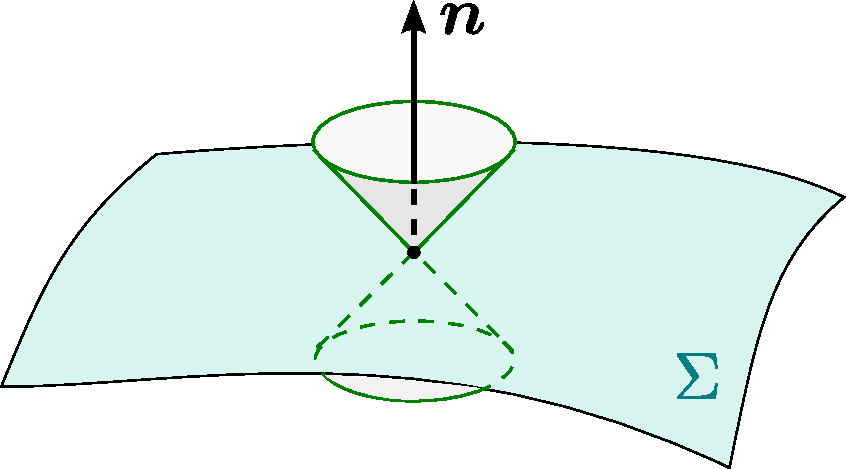
\includegraphics[width=0.45\textwidth]{def_spacelike_hyp.pdf}
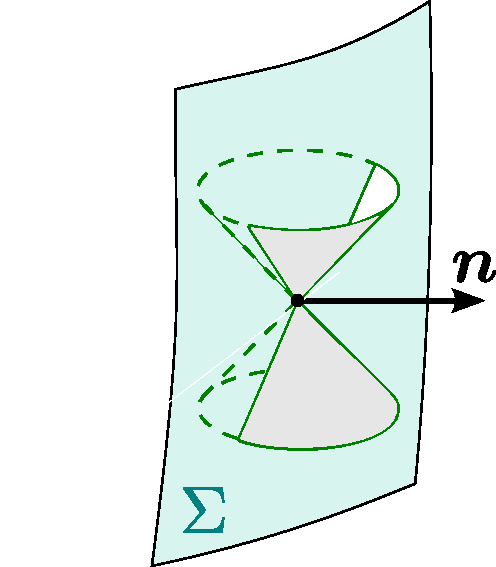
\includegraphics[width=0.25\textwidth]{def_timelike_hyp.pdf}
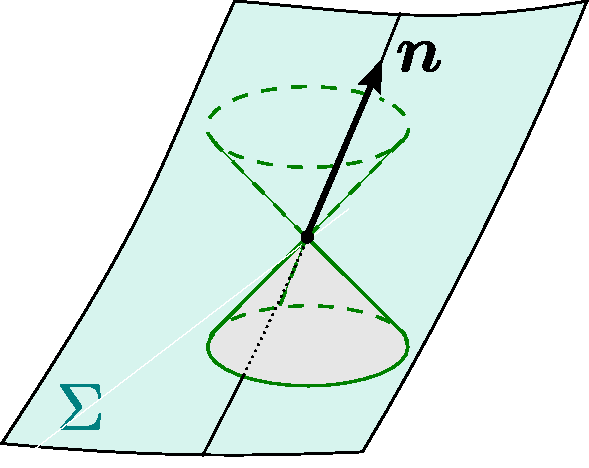
\includegraphics[width=0.30\textwidth]{def_null_hyp.pdf}}
\caption[]{\label{f:def:hypersurfaces} \footnotesize
The three types of hypersurfaces:
spacelike (left), timelike (middle) and null (right).}
\end{figure}

\subsection{The event horizon as a null hypersurface} \label{s:def:hor_as_null}

To discuss further which hypersurface could act as a black hole boundary,
one should recall that, on a Lorentzian manifold $(\M,\w{g})$, there are
three classes of hypersurfaces. The classification
depends on the type of metric induced by $\w{g}$ on the
hypersurface, $\Sigma$ say, the
\defin{induced metric}\index{induced!metric}\index{metric!induced --} being
nothing but the restriction $\left.\w{g}\right| _{\Sigma}$ of $\w{g}$
to vector fields tangent to $\Sigma$.
A hypersurface $\Sigma$ is said to be
\begin{itemize}
\item \defin{spacelike} iff $\left.\w{g}\right| _{\Sigma}$ is positive definite,
i.e. iff $\mathrm{sign} \left.\w{g}\right| _{\Sigma} = (+,+,+)$,
i.e. iff $(\Sigma,  \left.\w{g}\right| _{\Sigma})$ is a Riemannian manifold;
\item \defin{timelike} iff $\left.\w{g}\right| _{\Sigma}$ is a Lorentzian metric,
i.e. iff $\mathrm{sign} \left.\w{g}\right| _{\Sigma} = (-,+,+)$,
i.e. iff $(\Sigma,  \left.\w{g}\right| _{\Sigma})$ is a Lorentzian manifold;
\item \defin{null} iff $\left.\w{g}\right| _{\Sigma}$ is degenerate\footnote{
Cf. Sec.~\ref{s:bas:metric} in Appendix~\ref{s:bas} for the definition of a
degenerate bilinear form; the degeneracy
implies that the bilinear form $\left.\w{g}\right| _{\Sigma}$ is not,
strictly speaking, a metric on $\Sigma$.}
i.e. iff $\mathrm{sign} \left.\w{g}\right| _{\Sigma} = (0,+,+)$.
\end{itemize}
The hypersurface type can also be deduced from any normal vector\footnote{
The definition of a vector normal to a hypersurface is recalled in Sec.~\ref{s:bas:hyp_normal} of Appendix~\ref{s:bas}.}
$\w{n}$ to it (cf. Fig.~\ref{f:def:hypersurfaces}):
\begin{itemize}
\item $\Sigma$ spacelike $\iff$ $\w{n}$ timelike;
\item $\Sigma$ timelike $\iff$ $\w{n}$ spacelike;
\item $\Sigma$ null $\iff$ $\w{n}$ null.
\end{itemize}
These equivalences are easily proved by considering a $\w{g}$-orthogonal basis
adapted to $\Sigma$.

\begin{remark}
Null hypersurfaces have the distinctive feature that their normals are
also tangent to them. Indeed, by definition, the normal $\w{n}$ is null iff
$\w{n}\cdot\w{n}=0$, which is nothing but the condition
for $\w{n}$ to be tangent to $\Sigma$.
\end{remark}

\begin{figure}
\centerline{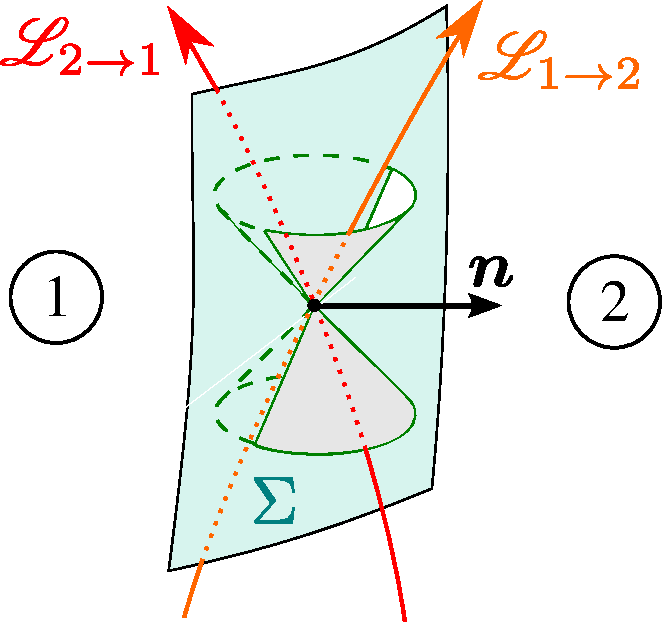
\includegraphics[width=0.4\textwidth]{def_timelike_2way.pdf}}
\caption[]{\label{f:def:timelike_2way} \footnotesize
A timelike hypersurface is a two-way membrane: $\Li_{1\rightarrow 2}$ is
a timelike worldline from Region~1 to Region~2, while $\Li_{2\rightarrow 1}$ is
a timelike worldline from Region~2 to Region~1.}
\end{figure}

\begin{figure}
\centerline{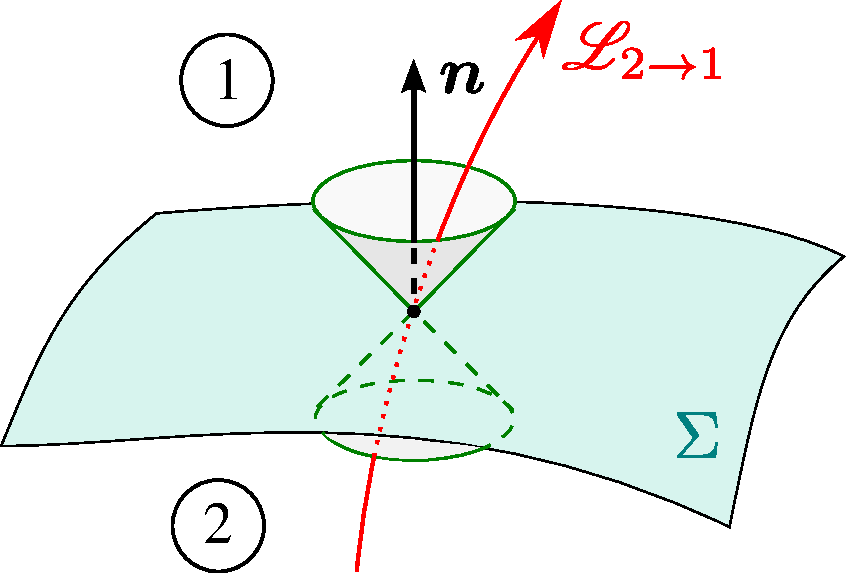
\includegraphics[width=0.5\textwidth]{def_spacelike_1way.pdf}}
\caption[]{\label{f:def:spacelike_1way} \footnotesize
A spacelike hypersurface is a one-way membrane: $\Li_{2\rightarrow 1}$ is
a timelike worldline from Region~2 to Region~1, while there is no timelike or null
worldline from Region~1 to Region~2.}
\end{figure}

\begin{figure}
\centerline{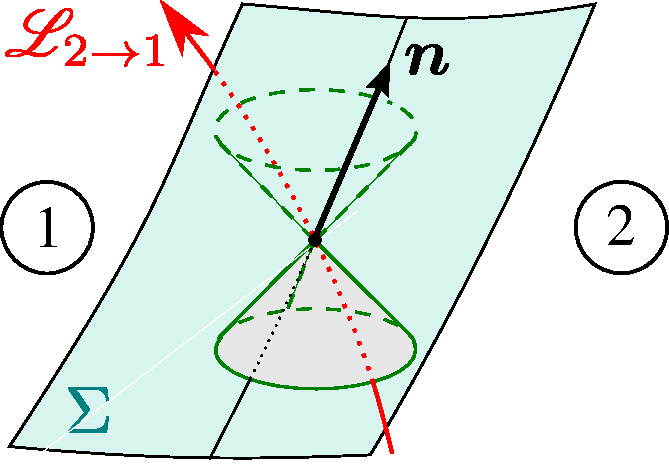
\includegraphics[width=0.5\textwidth]{def_null_1way.pdf}}
\caption[]{\label{f:def:null_1way} \footnotesize
A null hypersurface is a one-way membrane:: $\Li_{2\rightarrow 1}$ is
a timelike worldline from Region~2 to Region~1, while there is no timelike or null
worldline from Region~1 to Region~2.}
\end{figure}

A timelike hypersurface is a two-way membrane: if it divides (locally)
spacetime in two regions, 1 and 2 say, and a future-directed timelike or null
worldline can cross it from Region~1 to Region~2, or from Region~2 to Region~1
(see Fig.~\ref{f:def:timelike_2way}). On the contrary,
a spacelike hypersurface is a one-way membrane: a future-directed timelike or null
worldline, which is constrained to move inside the light cones,
can cross it only from Region~2 to Region~1, say (see Fig.~\ref{f:def:spacelike_1way}).
A null hypersurface is also a one-way membrane (see Fig.~\ref{f:def:null_1way}).
At most, a null worldline that is not going from Region~2 to Region~1 must
stay on the hypersurface; an exemple of such null wordline is
the one depicted in Fig.~\ref{f:def:null_1way} as the thin black line tangent to the normal $\w{n}$.

The limit case between two-way membranes (timelike hypersurfaces)
and one-way ones being null hypersurfaces, it is quite natural to select the
latter ones for the black hole boundary, rather than spacelike hypersurfaces.
This choice will be fully justified in Chap.~\ref{s:glo}, where we shall see
that the precise definition of a black hole implies that its boundary
(the event horizon\index{event!horizon}\index{horizon!event --})
is a null hypersurface as soon as it is smooth (Property~4 in Sec.~\ref{s:glo:properties_H}).
Note however that in Chap.~\ref{s:loc}, we shall see that spacelike hypersurfaces,
called \emph{dynamical
horizons}\index{dynamical!horizon}\index{horizon!dynamical --}, are involved
in quasi-local approaches to black holes.

%%%%%%%%%%%%%%%%%%%%%%%%%%%%%%%%%%%%%%%%%%%%%%%%%%%%%%%%%%%%%%%%%%%%%%%%%%%%%%%%

\section{Geometry of null hypersurfaces} \label{s:def:geom_null_hypsurf}

Having decided that the black hole event horizon must be a null hypersurface,
let us examine the geometrical properties of such hypersurfaces. We shall
denote the hypersurface under study by $\Hor$, for \emph{horizon}, but the results of this section
will be valid for any null hypersurface.

\subsection{Hypersurfaces as level sets}

As any hypersurface, $\Hor$ can be locally considered as a level set\index{level set}:
around any point of $\Hor$, there exists an open subset $\mathscr{U}$
of $\M$ (possibly  $\mathscr{U} = \M$) and
a smooth scalar field $u:\ \mathscr{U} \rightarrow \R$ such that
\be \label{e:def:Hor_u_zero}
    \forall p \in \mathscr{U},\quad p\in \Hor \iff u(p) = 0 .
\ee
and
\be \label{e:def:du_not_zero}
    \wnab u \not = 0 \quad \mbox{on}\ \Hor .
\ee
Condition (\ref{e:def:du_not_zero}) ensures that $\Hor$ is a regular
hypersurface (an \emph{embedded} submanifold, in mathematical terms); without it, $\Hor$ may have
self-intersection points.

\begin{figure}
\centerline{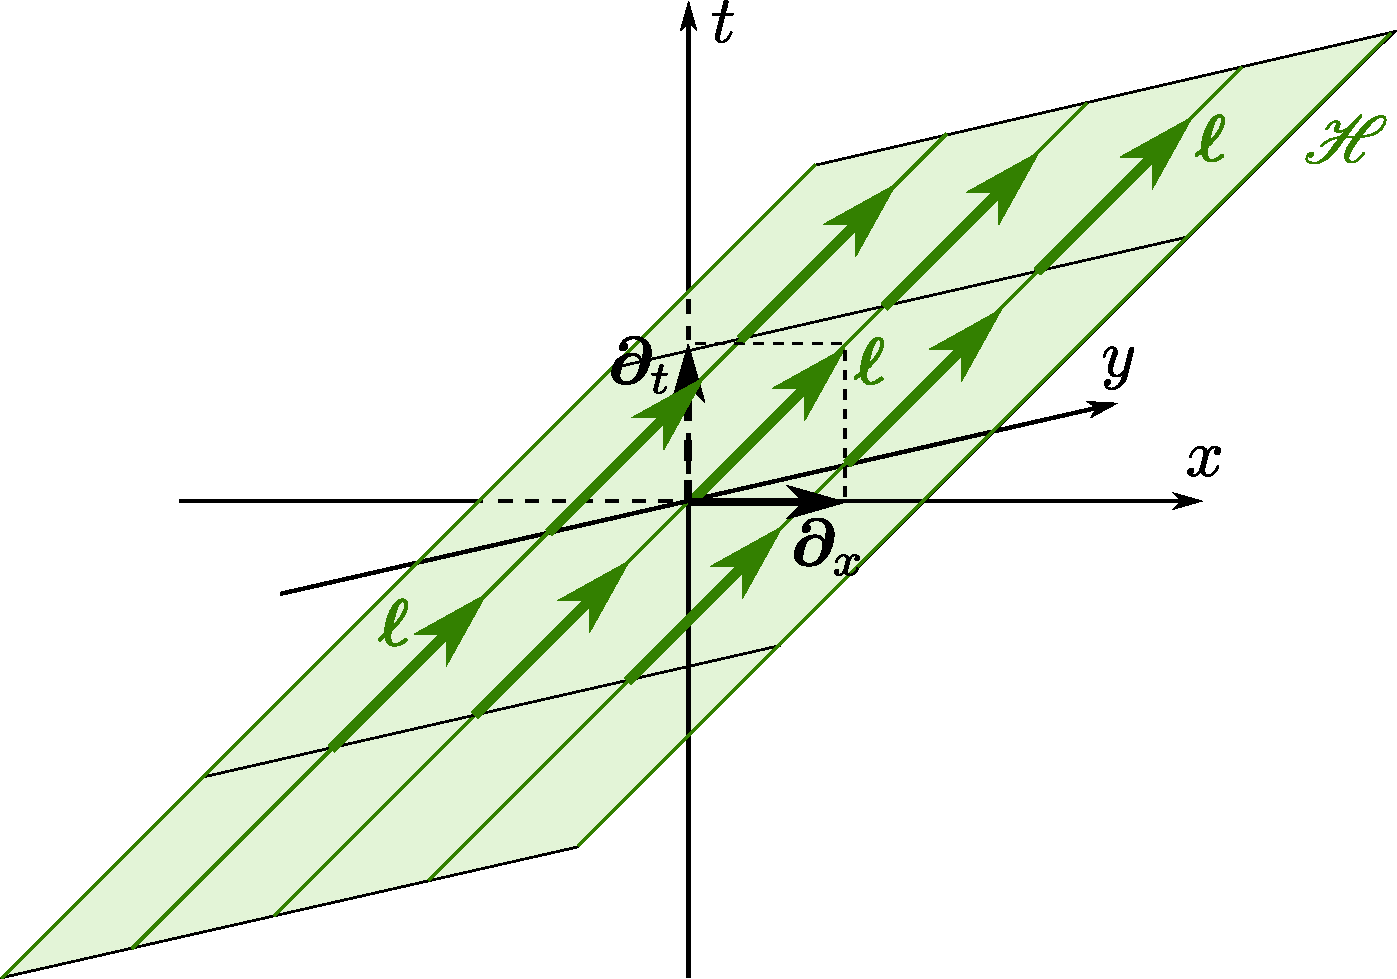
\includegraphics[width=0.6\textwidth]{def_null_hplane.pdf}}
\caption[]{\label{f:def:null_hplane} \footnotesize
Null hyperplane $\Hor$ of equation $t-x=0$ in Minkowski spacetime.
The dimension along $z$ has been suppressed, so that $\Hor$ is pictured as a
2-plane.}
\end{figure}


\begin{example}[null hyperplane] \label{x:def:null_hyp}
A very simple example of null hypersurface is a null hyperplane of
the 4-dimensional Minkowski spacetime. If $(t,x,y,z)$ are standard Minkowskian
coordinates, the choice of the scalar field
\be \label{e:def:null_plane_u}
    u(t,x,y,z) = t - x
\ee
defines a null hyperplane $\Hor$ by $u=0$ (cf. Fig.~\ref{f:def:null_hplane}).
\end{example}

\begin{example}[light cone] \label{x:def:light_cone}
Another simple example of null hypersurface, still in the 4-dimensional Minkowski spacetime,
is the future sheet $\Hor$ of a light cone\index{light!cone}\index{cone!light --}, also
called \defin{future light cone}\index{future!light cone}. Note that we have
to take out the cone apex from $\Hor$, in order to have a regular hypersurface.
In the  Minkowskian coordinates $(t,x,y,z)$, the choice of the
``retarded time''\index{retarded!time}
\be \label{e:def:light_cone_u}
    u(t,x,y,z) = t - \sqrt{x^2+y^2+z^2}
\ee
defines a future light cone $\Hor$ by $u=0$ and $t>0$ (cf.
Fig.~\ref{f:def:future_light_cone}).
\end{example}

\begin{figure}
\centerline{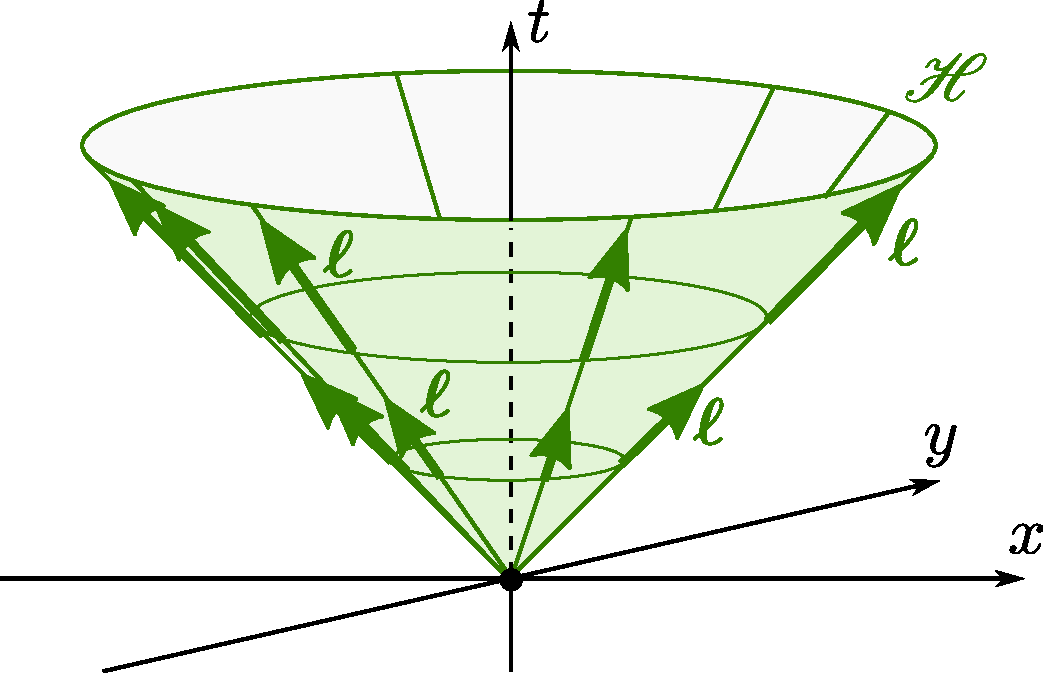
\includegraphics[width=0.6\textwidth]{def_future_light_cone.pdf}}
\caption[]{\label{f:def:future_light_cone} \footnotesize
Future sheet $\Hor$ of the light cone of equation $t-\sqrt{x^2+y^2+z^2}=0$ in Minkowski spacetime.
The dimension along $z$ has been suppressed, so that $\Hor$ looks 2-dimensional,
whereas it is actually 3-dimensional.}
\end{figure}


\begin{example}[Schwarzschild horizon] \label{x:def:Schw_hor}
Let us consider the 4-dimensional spacetime $(\M,\w{g})$ with $\M$ diffeomorphic
to $\mathbb{R}^4$ and equipped with a coordinate system $(x^\alpha)=(t,r,\th,\ph)$
($t\in \mathbb{R}$, $r\in(0,+\infty)$, $\th\in(0,\pi)$
and $\ph\in(0,2\pi)$) such that $\w{g}$ takes the form
\be \label{e:def:Schw_metric}
    g_{\mu\nu} \D x^\mu \D x^\nu = - \left( 1 - \frac{2 m}{r} \right) \D t^2
        + \frac{4m}{r} \, \D t \, \D r
        + \left( 1 + \frac{2 m}{r} \right) \D r^2
        + r^2\D\th^2 + r^2\sin^2\th \, \D\ph^2 ,
\ee
where $m$ is a positive constant. We shall see in Chap.~\ref{s:sch} that
$(\M,\w{g})$ is actually a part of Schwarzschild spacetime, described in
coordinates different from the standard Schwarzschild-Droste ones,  $(\bar t, r, \th, \ph)$
say, by the choice of the time coordinate:
$t = {\bar t} + 2m\ln|r/(2m)-1|$. The present coordinates are called
\defin{3+1 Eddington-Finkelstein coordinates}\index{Eddington-Finkelstein!coordinates}
and have the advantage over the the standard ones to be regular on the event horizon,
which is located at $r=2m$. Indeed, the metric components (\ref{e:def:Schw_metric})
remain finite when $r\rightarrow 2m$, as those of the inverse metric, which are
\be \label{e:def:Schw_metric_inv}
    g^{\alpha\beta} = \left(
    \begin{array}{cccc}
    - 1 - \frac{2m}{r} & \frac{2m}{r} & 0 & 0 \\
    \frac{2m}{r} & 1 - \frac{2m}{r} & 0 & 0 \\
    0 & 0 & \frac{1}{r^2} & 0 \\
    0 & 0 & 0 & \frac{1}{r^2\sin^2\th}
    \end{array} \right) .
\ee
Let us consider the scalar field defined on $\M$ by
\be \label{e:def:Schw_u}
    u(t,r,\th,\ph) = \left( 1 - \frac{r}{2m} \right)
            \exp\left(\frac{r-t}{4m}\right) .
\ee
It is then clear that the hypersurface $u=0$ is the
3-dimensional ``cylinder'' $\Hor$ of equation
$r=2m$ (cf. Fig.~\ref{f:def:Schwarz_horizon}). We shall see below\footnote{This should be obvious to the experienced
reader, since a normal 1-form to $\Hor$ is $\dd r$ and, from Eq.~(\ref{e:def:Schw_metric_inv}), $g^{rr}=0$ on $\Hor$.} that $\Hor$ is indeed a null hypersurface.
\end{example}

\begin{figure}
\centerline{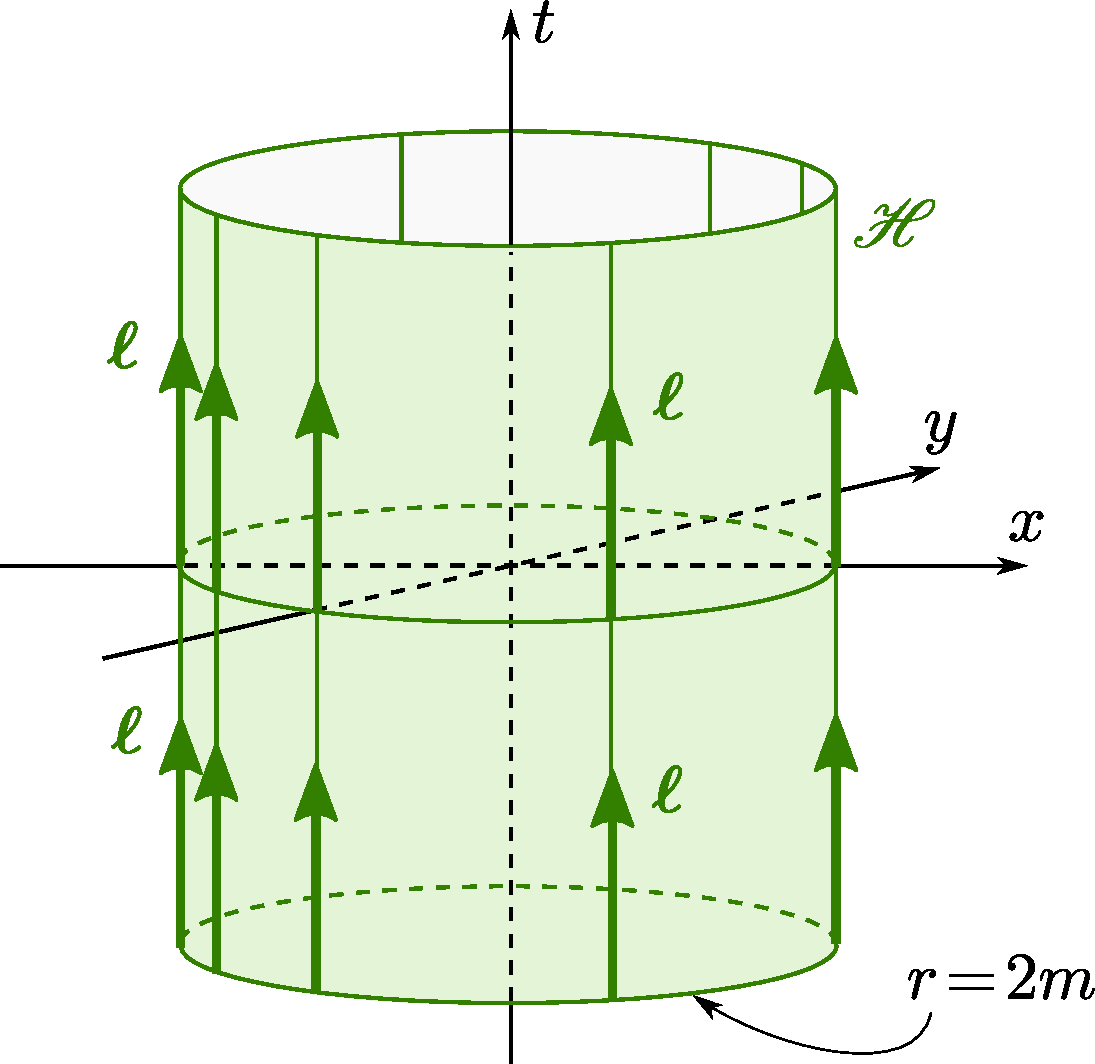
\includegraphics[width=0.5\textwidth]{def_Schwarz_horizon.pdf}}
\caption[]{\label{f:def:Schwarz_horizon} \footnotesize
Schwarzschild horizon $\Hor$ introduced in Example~\ref{x:def:Schw_hor};
The figure is drawn for $\th=\pi/2$ and is based on coordinates $(t,x,y)$
related to the 3+1 Eddington-Finkelstein coordinates $(t,r,\th,\ph)$
by $x=r\cos\ph$ and $y=r\sin\ph$.}
\end{figure}



\subsection{Null normals} \label{s:def:null_normal}

Let $\wl$ be a vector field normal to $\Hor$. Since $\Hor$ is a null hypersurface,
$\wl$ is a null vector:
\be \label{e:def:wl_null}
    \wl\cdot\wl = 0 .
\ee
Moreover, we choose $\wl$ to be future-directed (cf. Sec.~\ref{s:fra:spacetime}).

\begin{remark}
As a consequence of (\ref{e:def:wl_null}), there is no natural normalization
of $\wl$, contrary to the case of timelike or spacelike hypersurfaces,
where one can always choose the normal to be a unit vector
(scalar square equal to $1$ or $-1$). It follows that there is no unique choice
of $\wl$. At this stage, any rescaling $\wl \mapsto \wl' =  \alpha \wl$, with
$\alpha$ some strictly positive (to preserve the future orientation of $\wl$)
scalar field on $\Hor$,
yields a normal vector field $\wl'$ as valid as $\wl$.
\end{remark}
The null normal vector field $\wl$ is a priori defined on $\Hor$
only and not at points $p\not\in\Hor$.
However, it is worth to consider $\wl$ as a vector field
not confined to $\Hor$ but defined
in some open subset of $\M$ around $\Hor$.
In particular this would permit to define the spacetime covariant
derivative $\w{\nabla}\wl$, which is not possible if the
support of $\wl$ is restricted to $\Hor$.
Following Carter \cite{Carte97}, a simple way to achieve
this is to consider not only a single null hypersurface $\Hor$,
but a foliation of $\M$ (in the vicinity
of $\Hor$) by a family of null hypersurfaces, such that $\Hor$ is an
element of this family.
Without any loss of generality,
we may select the value of the scalar field $u$ defining $\Hor$ to label these hypersurfaces and
denote the family by $(\Hor_u)$. The null hypersurface $\Hor$
is then nothing but the element $\Hor = \Hor_{u=0}$ of this family
[Eq.~(\ref{e:def:Hor_u_zero})].
The vector field $\wl$ can then be viewed as being defined in the part of $\M$
foliated by $(\Hor_u)$, such that at each point in this region, $\wl$
is null and normal to $\Hor_u$ for some value of $u$.

\begin{example}
The scalar field $u$ introduced in Example~\ref{x:def:null_hyp}
(null hyperplane) does define a family of null hypersurfaces
$(\Hor_u)$. A counter-example would be $u(t,x,y,z)=(t-x)(1+x^2)$, since
$u=a$ does not define a null hypersurface except for $a=0$.
Similarly, the scalar fields $u$ of
Example~\ref{x:def:light_cone} (light cone)
and Example~\ref{x:def:Schw_hor} (Schwarzschild horizon)
do define a family of null
hypersurfaces $(\Hor_u)$. In the latter example, this would not have been the
case for the simpler choice $u(t,r,\th,\ph)  = r - 2m$.
\end{example}

Obviously the family $(\Hor_u)$ is non-unique but all geometrical
quantities that we shall introduce hereafter do not depend upon the choice
of the foliation $\Hor_u$ once they are evaluated at $\Hor$.

Since $\Hor$ is a hypersurface where $u$ is constant [Eq.~(\ref{e:def:Hor_u_zero})],
we have, by definition,
\bea
    \forall \w{v}\in T_p\M,\quad \w{v} \mbox{\ tangent to\ }\Hor & \iff  &
    \wnab_{\w{v}}\,  u = 0 \nonumber \\
    & \iff  & \langle \wnab u , \w{v} \rangle = 0 \nonumber \\
    & \iff & \vw{\nabla} u \cdot \w{v} = 0 ,   \label{e:def:nab_u_normal}
\eea
where $\vw{\nabla} u$ is the gradient vector field of the scalar field $u$,
i.e. the vector field given in index-notation by
\be \label{e:def:nab_up_u}
    \nabla^\alpha u = g^{\alpha\mu} \nabla_{\mu} u = g^{\alpha\mu} \der{u}{x^\mu} .
\ee
Property (\ref{e:def:nab_u_normal}) means that $\vw{\nabla} u$ is
a normal vector field to $\Hor$. By uniqueness of the normal direction to a hypersurface, it
must then be collinear to $\wl$. Therefore, there must exist some scalar
field $\rho$ such that
\be \label{e:def:wl_rho_u}
    \encadre{\wl = - e^\rho \, \vw{\nabla} u } .
\ee
We have chosen the
coefficient linking $\wl$ and $\vw{\nabla} u $ to be strictly negative,
i.e. under the form of minus an exponential. This is always possible by a suitable
choice of the scalar field $u$. The minus sign ensures that in the case
of $u$ increasing toward the future, $\wl$ is future-directed,
as the following example shows:

\begin{example}[null hyperplane] \label{x:def:null_hyp2}
We deduce from the
expression (\ref{e:def:null_plane_u}) chosen for $u$ in Example~\ref{x:def:null_hyp} that
\[
    \wnab u = \dd t - \dd x .
\]
The gradient vector field obtained by metric duality is
$\vw{\nabla} u = - \wpar_t - \wpar_x$. Choosing for simplicity $\rho=0$,
we get from formula~(\ref{e:def:wl_rho_u})
\be \label{e:def:wl_null_hyperplane}
    \wl =  \wpar_t + \wpar_x .
\ee
The vector field $\wl$ is depicted in Fig.~\ref{f:def:null_hplane}.
\end{example}

\begin{example}[light cone] \label{x:def:light_cone2}
Regarding Example~\ref{x:def:light_cone}, we have,
given expression (\ref{e:def:light_cone_u}) for $u$,
\[
    \wnab u = \dd t - \frac{x}{r} \dd x - \frac{y}{r} \dd y - \frac{z}{r} \dd z,
    \quad\mbox{with}\quad r:=\sqrt{x^2+y^2+z^2}.
\]
Choosing for simplicity $\rho=0$ in (\ref{e:def:wl_rho_u}), we get the
normal
\be \label{e:def:wl_light_cone}
    \wl = \wpar_t + \frac{x}{r} \wpar_x + \frac{y}{r} \wpar_y + \frac{z}{r} \wpar_z .
\ee
The vector field $\wl$ is depicted in Fig.~\ref{f:def:future_light_cone}.
\end{example}

\begin{example}[Schwarzschild horizon] \label{x:def:Schw_hor2}
We deduce from the expression (\ref{e:def:Schw_u}) chosen for $u$ in
Example~\ref{x:def:Schw_hor} that
\[
    \wnab u = \frac{1}{4 m} \mathrm{e}^{(r-t)/(4m)} \left[ - \left(1-\frac{r}{2m}  \right)
        \, \dd t
        - \left(1 + \frac{r}{2m}\right) \, \dd r \right] .
\]
The corresponding gradient vector field,
is computed from (\ref{e:def:nab_up_u}) via expression
(\ref{e:def:Schw_metric_inv}) for $g^{\alpha\mu}$:
\[
    \vw{\nabla} u = \frac{1}{4 m} \mathrm{e}^{(r-t)/(4m)} \left[
    - \left(1+ \frac{r}{2m} \right) \wpar_t
    + \left(1 - \frac{r}{2m} \right) \wpar_r \right] .
\]
This time, we do not chose $\rho=0$ but rather select $\rho$ so that
$\el^t = 1$:
\be \label{e:def:rho_Schw_hor}
    e^\rho =  - \frac{1}{\nabla^t u} \iff
    \rho = \frac{t-r}{4m} - \ln \left( 1 + \frac{r}{2m} \right) + \ln (4 m).
\ee
Equation~(\ref{e:def:wl_rho_u}) leads then to
\be \label{e:def:wl_Schw_hor}
    \wl = \wpar_t +  \frac{r-2m}{r+2m} \,  \wpar_r .
\ee
Given the metric (\ref{e:def:Schw_metric}), we check that $\w{g}(\wl, \wl)=0$.
Since $\wl\not=0$, this proves that all hypersurfaces $\Hor_u$, and in particular $\Hor$,
are null.
The vector field $\wl$ is depicted in Fig.~\ref{f:def:Schwarz_horizon}.
\end{example}

\subsection{Null geodesic generators}

\subsubsection{Frobenius identity}

Let us take the metric dual of relation (\ref{e:def:wl_rho_u}): it writes
$\uu{\el} = - e^\rho \, \wnab u$, or, in index notation,
\be
    \el_\alpha = - e^\rho \, \nabla_\alpha u .
\ee
Taking the covariant derivative, we get
\[
    \nabla_\alpha \el_\beta = - e^\rho \nabla_\alpha \rho \nabla_\beta u
                -   e^\rho  \nabla_\alpha \nabla_\beta u
                 = \nabla_\alpha \rho \, \el_\beta - e^\rho  \nabla_\alpha \nabla_\beta u
\]
Antisymmetrizing and using the torsion-free property of $\wnab$ (i.e.
$\nabla_\alpha \nabla_\beta u - \nabla_\beta \nabla_\alpha u = 0$, cf.
Eq.~(\ref{e:bas:torsion-free}) in Appendix~\ref{s:bas}), we get
\be \label{e:def:ext_der_wl_comp}
  \nabla_\alpha \el_\beta - \nabla_\beta \el_\alpha =
  \nabla_\alpha \rho \, \el_\beta -  \nabla_\beta \rho \, \el_\alpha  .
\ee
In the left-hand side there appears the exterior derivative of
the 1-form $\uu{\el}$ (cf. Sec.~\ref{s:bas:ext_deriv} in Appendix~\ref{s:bas}),
while one recognize in the right-hand side the exterior product of
the two 1-forms $\dd\rho$ and $\uu{\el}$. Hence we may rewrite (\ref{e:def:ext_der_wl_comp})
as
\be
    \encadre{ \dd \uu{\el} = \dd\rho \wedge \uu{\el} } .
\ee
This reflects the \defin{Frobenius theorem}\index{Frobenius!theorem}
in its dual formulation (see e.g.
Theorem B.3.2 in Wald's textbook \cite{Wald84}): the exterior derivative of
the 1-form $\uu{\el}$ is the exterior product of $\uu{\el}$ itself with some
1-form ($\dd\rho$ in the present case) if, and only if,
$\uu{\el}$ defines hyperplanes that are integrable in some hypersurface ($\Hor$ in the present case).

\subsubsection{Geodesic generators} \label{s:def:geod_gener}

Let us contract the Frobenius identity (\ref{e:def:ext_der_wl_comp}) with $\wl$:
\be \label{e:def:l_contract_Frob}
    \el^\mu \nabla_\mu \el_\alpha - \el^\mu \nabla_\alpha \el_\mu
        = \el^\mu \nabla_\mu \rho \, \el_\alpha
        - \underbrace{\el^\mu \el_\mu}_{0} \nabla_\alpha \rho .
\ee
Now, since $\wl$ is a null vector,
\[
    \el^\mu \nabla_\alpha \el_\mu = \nabla_\alpha (\underbrace{\el^\mu \el_\mu}_{0})
        - \el_\mu \nabla_\alpha \el^\mu ,
\]
from which we get
\be \label{e:def:el_nab_el_zero}
    \el^\mu \nabla_\alpha \el_\mu = 0 .
\ee
Hence (\ref{e:def:l_contract_Frob}) reduces to
\be \label{e:def:wl_geod_kappa_dual}
    \el^\mu \nabla_\mu \el_\alpha  = \kappa \, \el_\alpha ,
\ee
with
\be \label{e:def:def_kappa}
    \kappa := \el^\mu \nabla_\mu \rho = \wnab_{\wl}\,  \rho .
\ee
The metric dual of (\ref{e:def:wl_geod_kappa_dual}) is
\be \label{e:def:wl_geod_kappa}
    \encadre{ \wnab_{\wl}\, \wl = \kappa \, \wl } .
\ee
This equation implies that the field lines of $\wl$ are geodesics.
To demonstrate this, we note that a rescaling
\be \label{e:def:wl_rescale}
    \wl \mapsto \wl' =  \alpha \wl
\ee
with $\alpha$ a strictly positive scalar field can be performed to yield
a \defin{geodesic vector field}\index{geodesic!vector field} $\wl'$, i.e.
a vector field that obeys\footnote{A vector field that obeys the weaker condition
(\ref{e:def:wl_geod_kappa}) with $\kappa$ possibly different from zero is called
a \defin{pregeodesic vector field}\index{pregeodesic vector field}, cf. Remark~\ref{r:fra:geodesic_vector}
on page~\pageref{r:fra:geodesic_vector}.}
\be \label{e:def:wlp_geod}
    \wnab_{\wl'}\, \wl' = 0 .
\ee
\begin{proof}
Equations~(\ref{e:def:wl_rescale}) and
(\ref{e:def:wl_geod_kappa}) imply
\be \label{e:def:nab_lp_lp}
    \wnab_{\wl'}\, \wl' = \alpha\left(
        \wnab_{\wl}\, \alpha + \kappa \alpha \right) \wl .
\ee
Hence, since $\alpha>0$,
\[
    \wnab_{\wl'}\, \wl' = 0  \iff  \wnab_{\wl}\, \ln \alpha = -\kappa .
\]
Therefore it suffices to solve $\wnab_{\wl}\, \ln \alpha = -\kappa$, which
is a first-order ordinary differential equation along each field line of $\wl$,
to ensure that $\wl'$ is a geodesic vector field.
\end{proof}
Because of (\ref{e:def:wlp_geod}),
the field lines of $\wl'$ are  null geodesics and $\wl'$ is the tangent
vector to them associated with some affine parameter $\lambda$.
On the other side, if $\kappa\not=0$, $\wl$ is not a geodesic vector field
and therefore cannot be associated with some affine parameter. For this
reason the quantity $\kappa$ is called the
\defin{non-affinity coefficient}\index{non-affinity coefficient} of
the null normal $\wl$.

Since $\wl$ is collinear to $\wl'$, it obviously shares the same field lines,
which have just been shown to be null geodesics. These field lines are called the
\defin{null geodesic generators}\index{null!geodesic!generator}\index{generator!of a null hypersurface} of the hypersurface $\Hor$.

Hence, we have shown that
\begin{greybox}
Any null hypersurface $\Hor$ is ruled by a family of null geodesics, called the
\emph{generators of $\Hor$}, and each vector field $\wl$ normal to $\Hor$ is
tangent to these null geodesics.
\end{greybox}

\begin{remark}
\label{r:def:null_curves}
The above result is not trivial: while it is obvious that the field lines of the normal
vector field $\wl$ are null curves that are tangent to $\Hor$, the reader must
keep in mind that not all null curves are null geodesics. For instance, in
Minkowski spacetime, the helix defined in terms of
some Minkowskian coordinates $(x^\alpha)=(t,x,y,z)$ by the parametric equation
$x^\alpha(\lambda) = (\lambda, \cos\lambda, \sin\lambda, 0)$ is a null curve, i.e.
it has
a null tangent vector at each point, but it is not a null geodesics (in Minkowski
spacetime, all null geodesics are straight lines).
\end{remark}

As a by-product of (\ref{e:def:nab_lp_lp}), we get the behaviour of the
non-affinity coefficient under a rescaling of the null normal:
\be \label{e:def:rescale_kappa}
    \wl' = \alpha \wl \ \Longrightarrow \ \kappa' = \alpha \kappa + \wnab_{\wl} \alpha .
\ee

\begin{example}[null hyperplane] \label{x:def:null_hyp3}
It is clear on expression (\ref{e:def:wl_null_hyperplane}) for $\wl$ that
the covariant derivative
$\wnab \wl$ vanishes identically. In particular $\wnab_{\wl} \wl = 0$.
Equation~(\ref{e:def:wl_geod_kappa}) then implies
\be \label{e:def:kappa_0_nullhyp}
    \kappa = 0 ,
\ee
which is in agreement with Eq.~(\ref{e:def:def_kappa}) and the choice $\rho=0$
performed in Example~\ref{x:def:null_hyp2}. The null geodesic generators of $\Hor$ are the
straight lines defined by $t=x$, $y=y_0$ and $z=z_0$ for some constants
$(y_0,z_0)\in \mathbb{R}^2$.
They are depicted as green lines in Fig.~\ref{f:def:null_hplane}.
 Either $t$ or $x$ can be chosen as affine
parameters of these generators.
\end{example}

\begin{example}[light cone] \label{x:def:light_cone3}
From expression (\ref{e:def:wl_light_cone})
for $\wl$ and the fact that
$\nabla_\beta \el^\alpha = \partial_\beta \el^\alpha$
in the Minkowskian coordinates $(t,x,y,z)$, we get
\be \label{e:def:nab_l_light_cone}
    \nabla_\beta \el^\alpha = \left(
    \begin{array}{cccc}
    0 & 0 & 0 & 0 \\
    0 & \frac{y^2+z^2}{r^3} & - \frac{xy}{r^3} & - \frac{xz}{r^3} \\
    0 & - \frac{xy}{r^3} & \frac{x^2+z^2}{r^3} & - \frac{yz}{r^3} \\
    0 & - \frac{xz}{r^3} & - \frac{yz}{r^3} & \frac{x^2+y^2}{r^3}
    \end{array} \right)
    \qquad {(\alpha = \mbox{row index}; \atop \beta = \mbox{column index}).}
\ee
We obtain then $\el^\mu \nabla_\mu \el^\alpha = 0$.
From Eq.~(\ref{e:def:wl_geod_kappa}), we conclude that
\[
    \kappa = 0 ,
\]
which is in agreement with Eq.~(\ref{e:def:def_kappa}) and the choice $\rho=0$
performed in Example~\ref{x:def:light_cone2}. The null geodesic generators of $\Hor$
are the half-lines defined by $x=a t$, $y=b t$, $z = \sqrt{1-a^2-b^2} t$, with
$t>0$ and $(a,b)\in\mathbb{R}^2$ such that $a^2+b^2 \leq 1$.
They are depicted as green lines in Fig.~\ref{f:def:future_light_cone}.
Since from (\ref{e:def:wl_light_cone}) $\wnab_{\wl} t = 1$
and $\kappa=0$, $\lambda=t$ is an affine parameter along these null geodesic generators.
\end{example}

\begin{example}[Schwarzschild horizon] \label{x:def:Schw_hor3}
The covariant derivative of the vector field $\wl$ as given by (\ref{e:def:wl_Schw_hor})
is (cf. Appendix~\ref{s:sam} for the computation)
\be \label{e:def:nab_l_Schw_hor}
    \nabla_\beta \el^\alpha = \left(
    \begin{array}{cccc}
    \frac{m}{r^2} & \frac{m}{r^2} \frac{3r+2m}{r+2m} & 0 & 0 \\[1ex]
    \frac{m}{r^2}\frac{r-2m}{r+2m} & \frac{m}{r^2}\frac{3r^2-4m(r+m)}{(r+2m)^2} & 0 & 0 \\[1ex]
    0 & 0 & \frac{r-2m}{r(r+2m)} & 0 \\
    0 & 0 & 0 & \frac{r-2m}{r(r+2m)}
    \end{array} \right)
    \qquad {(\alpha = \mbox{row index}; \atop \beta = \mbox{column index}).}
\ee
Contracting with $\wl^\beta$, we obtain
\[
    \wnab_{\wl} \wl = \frac{4m}{(r+2m)^2} \wpar_t
        +  \frac{4m(r-2m)}{(r+2m)^3} \,  \wpar_r = \frac{4m}{(r+2m)^2}  \, \wl .
\]
Hence, for any $\Hor_u$, $\kappa=4m/(r+2m)^2$. On $\Hor$ ($r=2m$), we get
\be \label{e:def:kappa_Schw_hor}
   \kappa = \frac{1}{4m} .
\ee
This value agrees with $\kappa = \wnab_{\wl}\rho$ [Eq.~(\ref{e:def:def_kappa})] and the
choice (\ref{e:def:rho_Schw_hor}) made for $\rho$. Contrary to Examples~\ref{x:def:null_hyp3}
and \ref{x:def:light_cone3}, $\kappa$ does not vanish; hence $t$, which is
a parameter of the null geodesic generators associated with $\wl$ (since $\wnab_{\wl} t = 1$
by virtue of (\ref{e:def:wl_Schw_hor})),
is \emph{not} an affine parameter. The null geodesic generators are depicted
as vertical green lines in Fig.~\ref{f:def:Schwarz_horizon}.
\end{example}

\subsection{Cross-sections} \label{s:def:spacelike_sections}

Let us now focus on the first aspect of the black hole definition given
in Sec.~\ref{s:def:first_defin}: \emph{localization}.
This feature is crucial to distinguish a black hole boundary from other types
of null hypersurfaces. For instance the interior of a future null cone
in Minkowski spacetime is a region from which no particle may escape,
but since the null cone is expanding, particles can travel arbitrary far from
the centre. Therefore a null cone does not define a black hole.
A key parameter is hence the \emph{expansion} of null hypersurfaces, which we shall
discuss in the next section, after having introduced cross-sections.

\begin{figure}
\vspace{5cm}
%\centerline{\includegraphics[width=0.6\textwidth]{}}
\caption[]{\label{f:def:hor_cylinder} \footnotesize
The null hypersurface $\Hor$ and some cross-sections.}
\end{figure}

In the remaining of this chapter, we assume that the spacetime dimension
obeys $n\geq 3$. We define then a \defin{cross-section}\index{cross-section}
of the null hypersurface $\Hor$
as a submanifold $\Sp$ of $\Hor$ of codimension 2 (i.e. $\dim \Sp=n-2$),
such that (i) the null normal $\wl$ is nowhere tangent to $\Sp$ and (ii)
each null geodesic generator of $\Hor$ intersects $\Sp$ once, and only once.

\begin{notation}
Indices relative to a cross-section will range from $2$ to $n-1$ and
will be denoted by a Latin letter from the beginning of the alphabet: $a$, $b$, etc.
\end{notation}

To encompass the idea that an event horizon delimitates some
region of spacetime, we shall assume that the cross-sections
are \defin{closed manifolds}\index{closed!manifold}, i.e.
are compact without boundary. The simplest example is the sphere,
more precisely the $(n-2)$-dimensional sphere $\mathbb{S}^{n-2}$, where $n$
is the spacetime dimension. It is the one relevant for standard 4-dimensional
black holes. But at this stage, we shall allow for other
closed-manifold topologies, like that of a torus.

Given the definition of a cross-section $\Sp$,
the topology of $\Hor$ is then that of a ``tube'' or ``cylinder''
(cf. Fig.~\ref{f:def:hor_cylinder}):
\be \label{e:def:H_topology}
    \Hor \simeq \R \times \Sp.
\ee
For the standard 4-dimensional black holes, this is
$\Hor \simeq \R \times \mathbb{S}^{2}$.

A first important property of any cross-section $\Sp$ is to be spacelike,
i.e. every vector
tangent to $\Sp$ must be spacelike.
\begin{proof}
The spacelike character of $\Sp$ follows from the following
lemma\footnote{\emph{Exercise:} prove it!}:
\begin{greybox}
Every nonzero vector tangent to a null hypersurface is either spacelike or null.
Moreover, in the latter case, it is tangent to a null geodesic generator (i.e. it is normal
to the hypersurface).
\end{greybox}
Let $p \in \Sp$ and $\w{v}\in T_p\M$ be a nonzero vector tangent to $\Sp$.
The above lemma implies that $\w{v}$ is either spacelike or tangent to the
null geodesic generator $\Li$ going through $p$, but then $\Li$ would be tangent to $\Sp$,
which is not allowed, given the definition of a cross-section. We conclude
that $\w{v}$ is necessarily spacelike, which proves that $\Sp$ is a spacelike
submanifold.
\end{proof}

\begin{example}[light cone] \label{x:def:light_cone4}
From now on, we abandon the null hyperplane considered in Examples~\ref{x:def:null_hyp},
\ref{x:def:null_hyp2} and \ref{x:def:null_hyp3}, since its topology is $\mathbb{R}^3$,
and therefore not of the type (\ref{e:def:H_topology}) with $\Sp$ compact.
On the other side, the future sheet $\Hor$ of the light cone of Minkowski spacetime considered in Examples~\ref{x:def:light_cone},
\ref{x:def:light_cone2} and \ref{x:def:light_cone3} does obey (\ref{e:def:H_topology}),
since we have excluded the cone apex from $\Hor$.
A natural choice of cross-section is a sphere defined by $t=t_0$ for some positive constant $t_0$:
\[
    \Sp = \left\{ p \in \Hor,\  t(p) = t_0 \right\} .
\]
That $\Sp$ is a 2-dimensional sphere in the hyperplane $t=t_0$ is clear on its equation in terms
of the Minkowskian coordinates $(t,x,y,z)$:
\[
\Sp: \quad t=t_0 \quad\mbox{and}\quad x^2+y^2+z^2 = t_0^2,
\]
which follows immediately from $u=0$
[cf. Eq.~(\ref{e:def:light_cone_u})]. Moreover, this equation shows that the
radius of the sphere is $t_0$.
\end{example}

\begin{example}[Schwarzschild horizon] \label{x:def:Schw_hor4}
The 3-dimensional cylinder $\Hor$ introduced in Example~\ref{x:def:Schw_hor}
has the topology (\ref{e:def:H_topology}), with $\Sp\simeq \mathbb{S}^2$
(cf. Fig.~\ref{f:def:Schwarz_horizon}).
Since it is defined
by $r=2m$ in terms of the 3+1 Eddington-Finkelstein coordinates $(t,r,\th,\ph)$,
a natural coordinate system on $\Hor$ is $x^A = (t,\th,\ph)$. Moreover, we
have seen that the coordinate $t$ is the (non-affine) parameter of the null
geodesics generating $\Hor$ associated with the null normal $\wl$.
As in Example~\ref{x:def:light_cone4}, a natural choice of cross-section is a
sphere defined by $t=t_0$ for some constant $t_0$:
\[
    \Sp = \left\{ p \in \Hor,\  t(p) = t_0 \right\} .
\]
The equation of $\Sp$ in terms of the coordinates $(t,r,\th,\ph)$ is then
\[
    \Sp: \quad t=t_0 \quad\mbox{and}\quad r = 2m .
\]
Note that $x^a=(\th,\ph)$ constitutes a coordinate system on $\Sp$.
\end{example}

\begin{example}[binary black hole]
Some cross-sections of the event horizon $\Hor$ in numerically
generated binary black hole spacetimes are displayed in Figs.~\ref{f:glo:EH_headon}
and \ref{f:glo:EH_binspir} of Chap.~\ref{s:glo}.
\end{example}

Let us denote by $\w{q}$ the
\defin{metric induced on $\Sp$ by $\w{g}$}\index{induced!metric}\index{metric!induced --},
i.e. the bilinear form defined at any point $p\in\Sp$ by
\be \label{e:def:def_q_S}
    \forall (\w{u},\w{v})\in T_p\Sp\times T_p\Sp, \quad
     \w{q}(\w{u},\w{v}) = \w{g}(\w{u},\w{v}) .
\ee
Saying that $\Sp$ is spacelike is equivalent to saying that $\w{q}$ is
positive definite, i.e.
\be
    \forall \w{v}\in T_p\Sp,\quad
    \w{q}(\w{v},\w{v}) \geq 0 \quad \mbox{and} \quad
    \w{q}(\w{v},\w{v}) = 0 \iff \w{v} = 0.
\ee
In other words, $(\Sp, \w{q})$ is a \defin{Riemannian manifold}\index{Riemannian!manifold} (cf Sec.~\ref{s:bas:signature} in Appendix~\ref{s:bas}).

\begin{example}[Schwarzschild horizon] \label{x:def:Schw_hor4a}
The metric induced by $\w{g}$ on the cross-section
$\Sp$ of the Schwarzschild horizon defined in Example~\ref{x:def:Schw_hor4} is readily obtained by
setting $t=\mathrm{const}=t_0$ and $r=\mathrm{const}=2m$ in Eq.~(\ref{e:def:Schw_metric}),
since  $x^a=(\th,\ph)$ is a coordinate system on $\Sp$:
\be \label{e:def:q_S_Schw_hor}
    q_{ab} \D x^a \D x^b = 4m^2 \left( \D\th^2 + \sin^2\th \D^2\ph \right) .
\ee
\end{example}

\begin{figure}
\vspace{5cm}
%\centerline{\includegraphics[width=0.6\textwidth]{}}
\caption[]{\label{f:def:TS_ortho} \footnotesize
The tangent space to the cross-section $\Sp$ and its orthogonal complement.}
\end{figure}

An important consequence of $\Sp$ being spacelike is that, at each point
$p\in \Sp$, the tangent space $T_p\Sp$ has an orthogonal complement
$T_p^\perp\Sp$,  which is a timelike plane such that
$T_p\M$ is the direct sum of $T_p\Sp$ and $T_p^\perp\Sp$ :
\be \label{e:def:TM_direct_sum}
   \encadre{ \forall p\in \Sp,\quad T_p\M = T_p\Sp \oplus T_p^\perp\Sp }.
\ee
That $T_p^\perp\Sp$ is timelike is necessary for the signature of $\w{g}$
to be $(-,+,\ldots,+)$. This can be seen by constructing an $\w{g}$-orthogonal
basis of $T_p\M$ by the Gram-Schmidt process, starting form a
$\w{q}$-orthogonal basis of $T_p\Sp$. Since $\dim T_p\Sp = n-2$, we have
$\dim T_p^\perp\Sp = 2$, i.e. $T_p^\perp\Sp$ is a timelike 2-plane.
In other words, the metric induced by $\w{g}$ on
$T_p^\perp\Sp$ is Lorentzian:
\be
    \mathrm{sign}\, \left.\w{g}\right|_{T_p^\perp\Sp} = (-,+) .
\ee
By definition, the null normal $\wl$ is orthogonal to any vector
tangent to $\Sp$, i.e. $\wl \in T_p^\perp\Sp$.
Since $T_p^\perp\Sp$ is a timelike plane, it has two independent null directions,
which can be seen as the two intersections of the null cone at $p$ with
the 2-plane $T_p^\perp\Sp$ (cf. Fig.~\ref{f:def:TS_ortho}).
Let us denote by $\w{k}$ a future-directed null vector in the null direction of $T_p^\perp\Sp$
that is not along $\wl$. By a proper rescaling $\w{k}\mapsto \alpha\w{k}$,
we may choose $\w{k}$ so that
\be \label{e:def:k_el_minus_one}
        \w{k}\cdot\wl = -1 .
\ee
Given $\wl$ and $\Sp$, the condition (\ref{e:def:k_el_minus_one})
determines the null vector $\w{k}$ uniquely.
Since $\wl$ and $\w{k}$ are non-collinear vectors of $T_p^\perp\Sp$ and
$\dim T_p^\perp\Sp = 2$, they constitute a basis of $T_p^\perp\Sp$:
\be \label{e:def:TSperp_Span_k_l}
    T_p^\perp\Sp = \mathrm{Span}\left( \wl, \w{k} \right) .
\ee

A priori, the bilinear form $\w{q}$ is defined only on $T_p\Sp$, via (\ref{e:def:def_q_S}).
However, thanks to the orthogonal decomposition (\ref{e:def:TM_direct_sum}),
we can extend it to all vectors of $T_p\M$ by requiring
\be \label{e:def:q_zero_TSperp}
    \forall \w{v}\in T_p^\perp\Sp, \quad \w{q}(\w{v}, .) = 0 .
\ee
Indeed, given a pair $(\w{u},\w{v})$ of vectors in $T_p\M$, (\ref{e:def:TM_direct_sum})
implies that there are unique decompositions
\bea
  & & \w{u} = \w{u}^\parallel + \w{u}^\perp,\quad \mbox{with}\quad  \w{u}^\parallel \in T_p\Sp,
    \  \w{u}^\perp \in T_p^\perp\Sp \label{e:def:decomp_u} \\
  & & \w{v} = \w{v}^\parallel + \w{v}^\perp,\quad \mbox{with}\quad  \w{v}^\parallel \in T_p\Sp,
    \  \w{v}^\perp \in T_p^\perp\Sp .\label{e:def:decomp_v}
\eea
Then, using the bilinearity of $\w{q}$ and the property (\ref{e:def:q_zero_TSperp}),
we obtain
\be \label{e:def:q_all_vectors}
    \forall (\w{u},\w{v})\in T_p\M\times T_p\M, \quad
     \w{q}(\w{u},\w{v}) = \w{q}(\w{u}^\parallel,\w{v}^\parallel) .
\ee
Equation~(\ref{e:def:q_all_vectors}), along with (\ref{e:def:def_q_S}), can
be considered as the definition of $\w{q}$. An equivalent definition,
which provides an explicit expression of $\w{q}$, is
\be \label{e:def:q_g_k_l}
    \encadre{ \w{q} = \w{g} + \uu{\el}\otimes\uu{k} + \uu{k}\otimes\uu{\el} } ,
\ee
or, in index notation,
\[
    q_{\alpha\beta} = g_{\alpha\beta} + \el_\alpha k_\beta + k_\alpha \el_\beta .
\]
\begin{proof}
Let us show that (\ref{e:def:q_g_k_l}) implies
(\ref{e:def:q_all_vectors})-(\ref{e:def:def_q_S}).
Starting from (\ref{e:def:q_g_k_l}), we have for any pair of vectors $(\w{u},\w{v})$
in $T_p\M$,
\be \label{e:def:q_u_v_k_l}
    \w{q}(\w{u},\w{v}) = \w{u}\cdot\w{v} + (\wl\cdot\w{u})(\w{k}\cdot\w{v})
    + (\w{k}\cdot\w{u})(\wl\cdot\w{v}) .
\ee
Now, thanks to (\ref{e:def:TSperp_Span_k_l}), we may write the
orthogonal decompositions
(\ref{e:def:decomp_u})-(\ref{e:def:decomp_v}) as
\[
    \w{u} = \w{u}^\parallel + u^0 \wl + u^1 \w{k} \quad\mbox{and}\quad
    \w{v} = \w{v}^\parallel + v^0 \wl + v^1 \w{k} .
\]
Using $\wl\cdot\wl=0$, $\w{k}\cdot\w{k}=0$ and $\wl\cdot\w{k}=-1$
[Eq.~(\ref{e:def:k_el_minus_one})], we have then
\bea
 & & \w{u}\cdot\w{v} = \w{u}^\parallel \cdot\w{v}^\parallel - u^0 v^1 - u^1 v^0 \nonumber \\
 & & \wl\cdot\w{u} = -u^1, \quad \w{k}\cdot\w{u} = -u^0, \nonumber \\
 & & \wl\cdot\w{v} = -v^1, \quad \w{k}\cdot\w{v} = -v^0 .  \nonumber
\eea
Hence (\ref{e:def:q_u_v_k_l}) results in
\bea
    \w{q}(\w{u},\w{v}) & = & \w{u}^\parallel \cdot\w{v}^\parallel - u^0 v^1 - u^1 v^0
            + u^1 v^0 + u^0 v^1 \nonumber \\
                & = & \w{u}^\parallel \cdot\w{v}^\parallel,  \nonumber
\eea
which is nothing but (\ref{e:def:q_all_vectors}).
\end{proof}

\begin{example}[light cone] \label{x:def:light_cone5}
In continuation with Example~\ref{x:def:light_cone4}, the null
vector $\w{k}$ orthogonal to the sphere $\Sp$ and obeying $\w{k}\cdot\wl = -1$
is
\[
    \w{k} = \frac{1}{2} \wpar_t
        - \frac{x}{2r} \wpar_x - \frac{y}{2r} \wpar_y  - \frac{z}{2r} \wpar_z .
\]
Evaluating $\w{q}$ via (\ref{e:def:q_g_k_l}), given expression
(\ref{e:def:wl_light_cone}) for $\wl$, we get the following components
of $\w{q}$ with respect to the Minkowskian coordinates $x^\alpha=(t,x,y,z)$:
\[
    q_{\alpha\beta} = \left(
    \begin{array}{cccc}
    0 & 0 & 0 & 0 \\
    0 & \frac{y^2+z^2}{r^2} & - \frac{xy}{r^2} & - \frac{xz}{r^2} \\
    0 & - \frac{xy}{r^2} & \frac{x^2+z^2}{r^2} & - \frac{yz}{r^2} \\
    0 & - \frac{xz}{r^2} & - \frac{yz}{r^2} & \frac{x^2+y^2}{r^2}
    \end{array} \right) .
 \]
If we consider the spherical coordinates ${x'}^{\alpha}=(t,r,\th,\ph)$
deduced from the Minkowskian ones via the standard formulas:
\[
    \left\{ \begin{array}{l}
    x = r\sin\th\cos\ph \\
    y = r\sin\th\sin\ph \\
    z = r\cos\th
    \end{array} \right. ,
\]
the components of $\w{q}$ become instead
\be \label{e:def:q_light_cone_spher}
    {q'}_{\alpha\beta} = \left(
    \begin{array}{cccc}
    0 & 0 & 0 & 0 \\
    0 & 0 & 0 & 0 \\
    0 & 0 & r^2 & 0 \\
    0 & 0 & 0 & r^2\sin^2\th
    \end{array} \right) .
\ee
and we recognize in $q_{ab} = \mathrm{diag}(r^2, r^2 \sin^2\th)$ the
standard metric on the 2-sphere of radius $r$.
\end{example}

\begin{figure}
\centerline{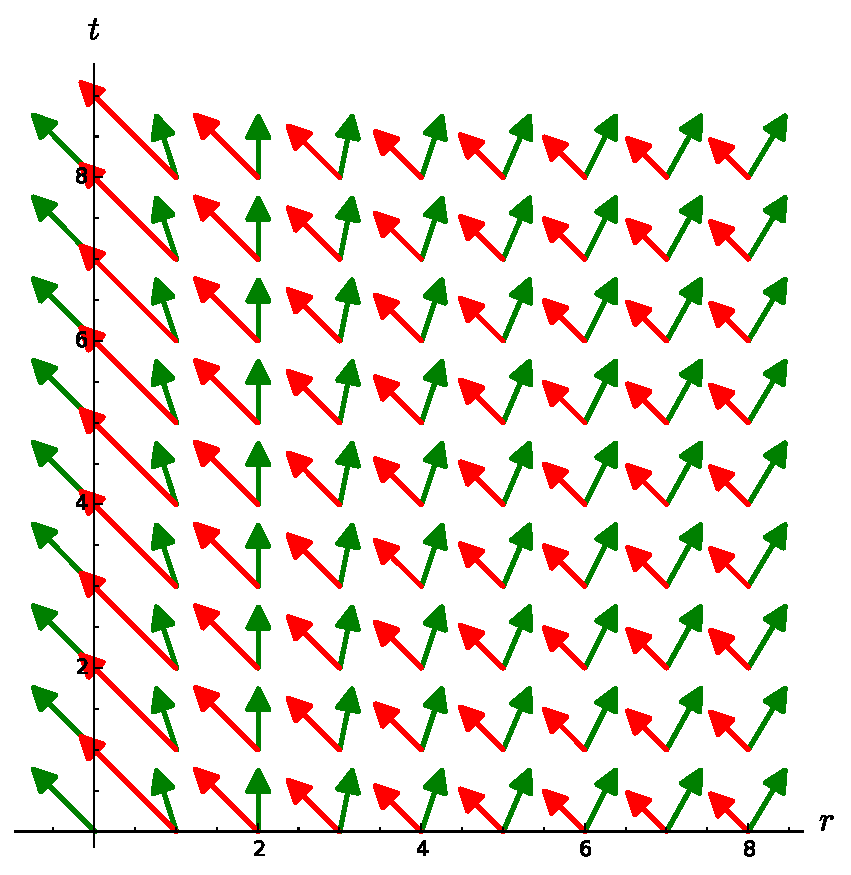
\includegraphics[width=0.6\textwidth]{def_plot_lk.pdf}}
\caption[]{\label{f:def:Schw_hor_lk} \footnotesize
Null vector fields $\wl$ (green) and $\w{k}$ (red) corresponding to
Example~\ref{x:def:Schw_hor5} (Schwarzschild horizon).
The plot is a 2-dimensional slice $\th=\mathrm{const}$ and $\ph=\mathrm{const}$
of the spacetime $\M$, with $t$ and $r$ labelled in units of $m$.
Note that
since $\w{k}$ diverges at $r=0$ [cf. Eq.~(\ref{e:def:k_Schw_hor})], it is not represented there.}
\end{figure}

\begin{example}[Schwarzschild horizon] \label{x:def:Schw_hor5}
For the Schwarzschild horizon case, we deduce from the metric (\ref{e:def:Schw_metric})
and the expression (\ref{e:def:wl_Schw_hor}) for $\wl$ that the null
vector $\w{k}$ orthogonal to the sphere $\Sp$ introduced
in Example~\ref{x:def:Schw_hor4} and obeying $\w{k}\cdot\wl = -1$
is
\be
\label{e:def:k_Schw_hor}
    \w{k} = \left(\frac{1}{2} + \frac{m}{r} \right) \wpar_t
        - \left(\frac{1}{2} + \frac{m}{r} \right) \wpar_r .
\ee
The vector field $\w{k}$ is depicted in Fig.~\ref{f:def:Schw_hor_lk}.
We have (cf. Appendix~\ref{s:sam})
\be \label{e:def:l_k_forms_Schw_hor}
    \uu{\el} = \frac{2m-r}{2m+r} \, \dd t  + \dd r
    \qquad\mbox{and}\qquad
    \uu{k} = - \left(\frac{1}{2} + \frac{m}{r} \right) \dd t
        - \left(\frac{1}{2} + \frac{m}{r} \right) \dd r ,
\ee
so that Eq.~(\ref{e:def:q_g_k_l}) leads to the following components of $\w{q}$
in terms of the 3+1 Eddington-Finkelstein coordinates $x^\alpha=(t,r,\th,\ph)$:
\be \label{e:def:q_Schw_hor}
    q_{\alpha\beta} = \left(
    \begin{array}{cccc}
    0 & 0 & 0 & 0 \\
    0 & 0 & 0 & 0 \\
    0 & 0 & r^2 & 0 \\
    0 & 0 & 0 & r^2\sin^2\th
    \end{array} \right) .
\ee
\end{example}

Having extended the definition of $\w{q}$ via (\ref{e:def:q_g_k_l}), we notice
that the metric dual\footnote{See Eq.~(\ref{e:bas:arrow_endo}) of
Appendix~\ref{s:bas} for the explanation of the arrow notation.}
 of $\w{q}$, i.e. the tensor of type $(1,1)$ defined by
by
\be \label{e:def:q_proj}
    \vw{q} := \mathrm{Id} + \wl\otimes \uu{k} + \w{k}\otimes \uu{\el},
\ee
or, in index notation,
\[
    q^\alpha_{\ \, \beta} = \delta^\alpha_{\ \, \beta}
        + \el^\alpha \, k_\beta + k^\alpha \, \wl_\beta ,
\]
is nothing but the \defin{orthogonal projector} onto the cross-section $\Sp$:
\be
    \forall \w{v}\in T_p\M, \quad \vw{q}(\w{v}) = \w{v}^\parallel .
\ee
The demonstration follows from the decomposition
$\w{v} = \w{v}^\parallel + v^0 \wl + v^1 \w{k}$ used above.
In particular, we have
\be
    \vw{q}(\wl) = 0 \quad\mbox{and}\quad \vw{q}(\w{k}) = 0 .
\ee

%%%%

As stressed by (\ref{e:def:TSperp_Span_k_l}), $(\wl,\w{k})$ forms a null
basis\index{null!basis}\index{basis!null --} of $T_p^\perp\Sp$. One can construct
from it an \emph{orthonormal} basis $(\w{n},\w{s})$ as follows:
\be \label{e:def:ns_lk}
    \left\{ \begin{array}{lcl}
        \w{n} & = & \frac{1}{2} \wl + \w{k} \\
        \w{s} & = & \frac{1}{2} \wl - \w{k} .
        \end{array}\right.
\ee
This system is easily inverted:
\be \label{e:def:lk_ns}
    \left\{ \begin{array}{lcl}
        \wl & = & \w{n} + \w{s} \\
        \w{k} & = & \frac{1}{2} \left( \w{n} - \w{s} \right).
        \end{array}\right.
\ee
Since $\wl\cdot\wl=0$, $\w{k}\cdot\w{k}=0$ and $\wl\cdot\w{k}=-1$, it is
easy to check that:
\be
    \w{n}\cdot\w{n}=-1,\quad \w{s}\cdot\w{s}=1 \quad\mbox{and}\quad
    \w{n}\cdot\w{s}=0.
\ee
In other words, $(\w{n},\w{s})$ is an orthonormal basis\index{orthonormal!basis}\index{basis!orthonormal --} of
the Lorentzian plane $(T_p^\perp\Sp,\w{g})$; in particular:
\be
    T_p^\perp\Sp = \mathrm{Span}\left( \w{n}, \w{s} \right) .
\ee

If we substitute (\ref{e:def:lk_ns}) for $\wl$ and $\w{k}$ in (\ref{e:def:q_g_k_l}),
we get
\[
    \w{q} = \w{g} + \frac{1}{2} (\uu{n}+\uu{s})\otimes(\uu{n}-\uu{s})
    + \frac{1}{2} (\uu{n}-\uu{s})\otimes(\uu{n}+\uu{s}) .
\]
Expanding and simplifying results in
\be
    \w{q} = \w{g} + \uu{n}\otimes\uu{n} - \uu{s}\otimes\uu{s} .
\ee

\begin{figure}
\centerline{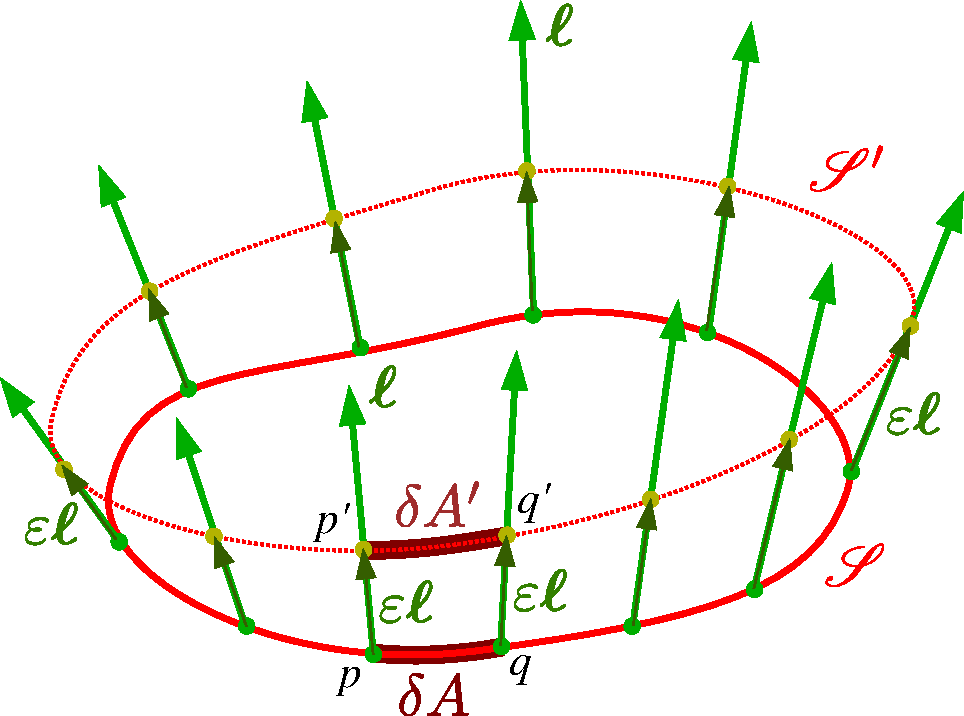
\includegraphics[width=0.6\textwidth]{def_expansion.pdf}}
\caption[]{\label{f:def:expansion} \footnotesize
Lie dragging of the surface $\Sp$ along $\wl$ by the small parameter $\varepsilon$.
$\Sp$ is drawn as a 1-dimensional submanifold, while it is actually a
$(n-2)$-dimensional one, $n$ being the spacetime dimension.}
\end{figure}

\subsection{Expansion along the null normal}

Let us define the expansion of the cross-section $\Sp$ along the vector
field $\wl$ as follows. Given an infinitesimal parameter $\varepsilon\geq 0$, take a point
$p\in \Sp$ and displace it by the (infinitesimal) vector $\varepsilon \wl$, thereby getting
a nearby point $p_\varepsilon$ (cf. Fig.~\ref{f:def:expansion}).
Since $\wl$ is tangent to $\Hor$ and $p\in\Hor$, we have $p_\varepsilon\in\Hor$.
By repeating this for each point in $\Sp$,
keeping the value of $\varepsilon$ fixed, we define a new codimension-2 surface,
$\Sp_\varepsilon$ say cf. Fig.~\ref{f:def:expansion}). One says that $\Sp_\varepsilon$ is obtained
from $\Sp$ by \defin{Lie dragging along $\wl$ by the parameter $\varepsilon$}\index{Lie!dragging}.
Note that $\Sp_0 = \Sp$.
Since $p_\varepsilon\in\Hor$ for every $p\in\Sp$, we have $\Sp_\varepsilon\subset \Hor$.
Because the null direction $\wl$ is transverse to $\Sp_\varepsilon$ by construction, it
follows that $\Sp_\varepsilon$ is spacelilke (cf. the lemma in Sec.~\ref{s:def:spacelike_sections}).

At each point $p\in\Sp$, the \defin{expansion of $\Sp$ along $\wl$} is defined from the
rate of change $\theta_{(\wl)}$ of the area\footnote{We are using the words
\emph{area} and \emph{surface} even if $n-2 \not= 2$, i.e. even if $n\not = 4$,
being aware that for $n=3$ the words \emph{length} and \emph{line} would
be more appropriate, as well as \emph{volume} for $n=5$.}
 $\delta A$ of an element of surface $\delta S$ of
$\Sp$ around $p$:
\be \label{e:def:def_expansion}
    \encadre{ \theta_{(\wl)} := \lim_{\varepsilon\rightarrow 0} \frac{1}{\varepsilon}
    \frac{\delta A_\varepsilon - \delta A}{\delta A} }.
\ee
In the above formula, $\delta A_\varepsilon$ stands for the area of the
surface element $\delta S_\varepsilon\subset \Sp_\varepsilon$ that is obtained from $\delta S$ by
Lie dragging along $\wl$ by the parameter $\varepsilon$ (cf. Fig.~\ref{f:def:expansion}).
\begin{remark} \label{r:def:expansion_indpt_S}
The reader may wonder why the expansion is not denoted by something like
$\theta_{(\wl)}(\Sp)$, since its definition depends explicitly on
$\Sp$. We shall show below that, because $\Hor$ is a null hypersurface, $\theta_{(\wl)}$
is actually independent of the choice of the cross-section $\Sp$.
\end{remark}

For concreteness, let us assume that the element of surface $\delta S \subset\Sp$ is a $(n-2)$-dimensional
parallelogram delimited by some infinitesimal displacement vectors
$\D\w{x}_{(2)}$, $\ldots$, $\D\w{x}_{(n-1)}$. The area of $\delta S$ is then
\be \label{e:def:A_wepsS_dx}
    \delta A = \wepsS(\D\w{x}_{(2)},\ldots,\D\w{x}_{(n-1)}),
\ee
where $\wepsS$ is the Levi-Civita tensor\index{Levi-Civita!tensor}
associated with the metric $\w{q}$
in $\Sp$ (cf. Sec.~\ref{s:bas:Levi-Civita_tensor} in Appendix~\ref{s:bas}).
Since $\w{q}$ is the metric induced by $\w{g}$ in $\Sp$ and $(\w{n},\w{s})$
is an orthonormal basis of $T_p^\perp \Sp$, $\wepsS$ is actually the
alternating form induced on $\Sp$ by the spacetime Levi-Civita tensor
$\weps$:
\be \label{e:def:epsS_ns}
    \encadre{ \wepsS = \weps(\w{n},\w{s},\ldots) },
\ee
or, in index notation,
\[
    \epsS_{\alpha_1\cdots\alpha_{n-2}} = \eps_{\mu\nu\alpha_1\cdots\alpha_{n-2}} n^\mu s^\nu .
\]
\begin{proof}
To demonstrate (\ref{e:def:epsS_ns}), it suffices to note that its right-hand side
defines a fully antisymmetric $(n-2)$-linear form on $T_p\Sp$. Since the space
of such forms is 1-dimensional (for $\dim T_p\Sp = n-2$), we have then
necessarily $\weps(\w{n},\w{s},\ldots) = a \wepsS$ for some proportionality factor $a$. Since
$\weps(\w{n},\w{s},\D\w{x}_{(2)},\ldots,\D\w{x}_{(n-1)})$ is the volume
of the $n$-parallelepiped constructed on the vectors $\w{n},\w{s},\D\w{x}_{(2)},\ldots,\D\w{x}_{(n-1)}$ and $\w{n}$ and $\w{s}$ are unit-length vectors for the metric $\w{g}$,
we have
\[
    \weps(\w{n},\w{s},\D\w{x}_{(2)},\ldots,\D\w{x}_{(n-1)}) = \delta A.
\]
This implies that $a=1$, thereby establishing (\ref{e:def:epsS_ns}).
\end{proof}
An alternative expression of $\wepsS$ is obtained by substituting (\ref{e:def:ns_lk})
for $\w{n}$ and $\w{s}$ in (\ref{e:def:epsS_ns}). Thanks to the multilinearity
and antisymmetry of $\weps$, we get
\be
    \encadre{ \wepsS = \weps(\w{k},\wl,\ldots) } .
\ee

Let us consider in some vicinity of $\Sp$ a coordinate system
\[
    x^\alpha = \left(\varepsilon, u, x^2,\ldots, x^{n-1}\right)
\]
that is adapted to $\Sp$ and $\wl$ in the sense that
\be \label{e:def:l_dsdeps}
    \wl = \der{}{\varepsilon}
\ee
and the points of $\Sp$ are defined by $(\varepsilon,u) = (0,0)$.
Then, from the very definition of the Lie dragging of $\Sp$ along $\wl$, we
have
\be
    \Sp_\varepsilon = \left\{ p\in\M,\quad  (x^0(p), x^1(p)) = (\varepsilon,0)
                        \right\}
\ee
and  $x^a = (x^2,\ldots, x^{n-1})$ can  be viewed as a coordinate system\footnote{
Let us recall that according to the convention stated in Sec.~\ref{s:def:spacelike_sections},  Latin indices from the beginning of the alphabet, $a$, $b$, etc. range from $2$
to $n-1$.} on each surface $\Sp_\varepsilon$.
Let us choose the $n-2$ infinitesimal displacement vectors in (\ref{e:def:A_wepsS_dx})
along the coordinate lines of this system:
\be
    \D x_{(i)}^a = (\underbrace{0,\ldots,0}_{i-2},\D x^i,
                    \underbrace{0,\ldots,0}_{n-1-i}), \qquad
                    2\leq i \leq n-1 .
\ee
Then expression~(\ref{e:def:A_wepsS_dx}) for the area of $\delta S$ becomes
\bea
    \delta A & = & \epsS_{a_1 \cdots a_{n-2}} \, \D x_{(2)}^{a_1} \cdots \D x_{(n-1)}^{a_{n-2}}
                    \nonumber \\
            & = & \epsS_{2\cdots(n-1)} \, \D x^2 \cdots \D x^{n-1} \nonumber \\
     \delta A  & = & \sqrt{q} \, \D x^2 \cdots \D x^{n-1} , \label{e:def:A_sqrt_q}
\eea
where we have used (\ref{e:bas:eps_sqrt_g}) for the components of the
Levi-Civita tensor $\wepsS$, $q$ standing for the determinant of the metric
$\w{q}$ with respect to the coordinates $(x^2,\ldots,x^{n-1})$.
By the very definition of the Lie dragging, the surface element
$\delta S_\varepsilon$ on $\Sp_\varepsilon$
is defined by the same values of the coordinates $(x^2,\ldots, x^{n-1})$
as $\delta S$. In particular, the small coordinate increments $\D x^2$, ..., $\D x^{n-1}$
take the same values as on $\Sp$. Therefore, the area of $\delta S_\varepsilon$
is
\be \label{e:def:A_eps_sqrt_q}
    \delta A_\varepsilon = \sqrt{q(\varepsilon)} \, \D x^2 \cdots \D x^{n-1} ,
\ee
where $q(\varepsilon)$ stands for the determinant of the components of the
metric $\w{q}(\varepsilon)$ induced by $\w{g}$ on $\Sp_\varepsilon$. Since
$\Sp_\varepsilon$ is spacelike (cf. above), $\w{q}(\varepsilon)$ is positive definite, so
that $q(\varepsilon)\geq 0$.

In view of (\ref{e:def:A_sqrt_q})-(\ref{e:def:A_eps_sqrt_q}), the definition (\ref{e:def:def_expansion})
of the expansion of $\Sp$ along $\wl$ can be rewritten as
\[
    \theta_{(\wl)} = \lim_{\varepsilon\rightarrow 0} \frac{1}{\varepsilon}
    \frac{\sqrt{q(\varepsilon)} - \sqrt{q(0)}}{\sqrt{q(0)}} .
\]
We recognize the derivative of the function $\varepsilon \mapsto \ln \sqrt{q(\varepsilon)}=
1/2\, \ln q(\varepsilon)$ at $\varepsilon=0$:
\be \label{e:def:theta_deps_ln_q}
     \theta_{(\wl)} = \frac{1}{2} \frac{\D}{\D\varepsilon}  \ln q .
\ee
Given that $\Sp_\varepsilon$ is deduced from $\Sp$ by a Lie dragging along $\wl$
and $\varepsilon$ is the parameter associated with $\wl$ [cf. Eq.~(\ref{e:def:l_dsdeps})], we may
rewrite this formula as the Lie derivative of $\ln q$ along $\wl$:
\be \label{e:def:theta_Lie_ln_q}
    \encadre{ \theta_{(\wl)} = \frac{1}{2} \Lie{\el} \ln q }.
\ee
\begin{example}[light cone] \label{x:def:light_cone6}
For the light cone in Minkowski spacetime,
it is easy to evaluate $\theta_{(\wl)}$ by means of the spherical coordinates
introduced in Example~\ref{x:def:light_cone5}, since these coordinates are adapted to the
surface $\Sp$, the metric of $\Sp$ being $q_{ab} \D x^a \D x^b = r^2 \D \theta^2
+ r^2\sin^2\theta \D \ph^2$ [cf. Eq.~(\ref{e:def:q_light_cone_spher})].
We have then  $q = \det(q_{ab}) = r^4\sin^2\theta$. Moreover the parameter $\varepsilon$
can be chosen as $\varepsilon = t - t_0$ since $t$ is an (affine) parameter
associated with $\wl$ (cf. Example~\ref{x:def:light_cone3}). Given that
$t=r$ on $\Hor$, we have $\varepsilon = r - t_0$, so that (\ref{e:def:theta_deps_ln_q})
yields
\[
    \theta_{(\wl)} = \frac{1}{2} \frac{\D}{\D r}  \ln q =
         \frac{1}{2} \frac{\D}{\D r} \left( 4 \ln r + 2 \ln\sin\theta \right) ,
\]
i.e.
\be \label{e:def:theta_light_cone}
    \theta_{(\wl)} = \frac{2}{r} .
\ee
\end{example}

\begin{example}[Schwarzschild horizon] \label{x:def:Schw_hor6}
As above, we have $q = r^4\sin^2\th$ [cf. Eq.~(\ref{e:def:q_S_Schw_hor})],
so that (\ref{e:def:theta_Lie_ln_q}) yields
\bea
    \theta_{(\wl)} & =& \frac{1}{2} \Lie{\el} \ln q = \frac{1}{2} \el^\mu \der{}{x^\mu} \ln q
        = \underbrace{\der{}{t} \ln (r^2\sin\th)}_{0}
            + \frac{r-2m}{r+2m} \der{}{r} \ln (r^2\sin\th) \nonumber \\
       & = & \frac{2}{r} \frac{r-2m}{r+2m}  . \label{e:def:theta_Schw_hor_u}
\eea
where we have used
(\ref{e:def:wl_Schw_hor}) for the components $\el^\mu$.
The above expression is valid for any null hypersurface $\Hor_u$. For the
specific case of the Schwarzschild horizon, $r=2m$ and (\ref{e:def:theta_Schw_hor_u})
yields a vanishing expansion:
\be \label{e:def:theta_Schw_hor}
    \theta_{(\wl)} = 0 .
\ee
Note that for large $r$, Eq.~(\ref{e:def:theta_Schw_hor_u}) yields
$\theta_{(\wl)} \sim 2/r$, i.e. we recover the flat
spacetime result (\ref{e:def:theta_light_cone}), which is consistent with the
fact that for large $r$, $\Hor_u$ is closed to a Minkowskian light cone
(cf. Fig.~??). Note also that Eq.~(\ref{e:def:theta_Schw_hor_u}) yields
$\theta_{(\wl)} <0$ for $r<2m$ and $\theta_{(\wl)} >0$ for $r>2m$. These
expansion values are in agreement with what can be infered from Fig.~\ref{f:def:Schw_hor_lk},
since $r$ is directly related to the area of the cross-sections of $\Hor$:
$A = 4\pi r^2$ from Eq.~(\ref{e:def:q_Schw_hor}).
\end{example}

Using the general law of variation of a derminant, as given by Eq.~(\ref{e:bas:variation_det})
in Appendix~\ref{s:bas}, Eq.~(\ref{e:def:theta_Lie_ln_q}) can be rewritten as
\[
    \theta_{(\wl)} = \frac{1}{2} \, \mathrm{tr} \left(Q^{-1} \times \Lie{\el} Q \right) ,
\]
when $Q$ is the matrix representing the components of $\w{q}$ with respect to the
coordinates $(x^a) = (x^2,\ldots, x^{n-1})$. In index notation, we have
$Q = (q_{ab})$ and $Q^{-1} = (q^{ab})$. Hence
\be \label{e:def:theta_q_ab}
    \encadre{ \theta_{(\wl)} = \frac{1}{2} \, q^{ab} \Liec{\el} q_{ab} } .
\ee
One may wonder about the link between the Lie derivative along $\wl$ of the $(n-2)$-metric
$\w{q}$ of the cross-sections $\Sp_\varepsilon$, which appears above, and
the Lie derivative along $\wl$ of the spacetime extension $\w{q}$ defined by
(\ref{e:def:q_g_k_l}). For the sake of clarity, let us denote here the latter
by $\w{\bar q}$. More precisely, we may consider that $\w{\bar q}$ is a
field defined in some neighbourhood of the portion of $\Hor$ sliced by
$\bigcup_{\varepsilon} \Sp_\varepsilon$ via (\ref{e:def:q_g_k_l}), with $\w{k}$
defined at each point $p\in\Sp_\varepsilon$ as the unique null vector of
$T_p^\perp\Sp_\varepsilon$ obeying $\wl\cdot\w{k}=-1$.
Let $\w{u}$ and $\w{v}$ be vector fields on $\Hor$ that are tangent
to the cross-sections $\Sp_\varepsilon$. Applying the bilinear form
$\Lie{\el}\w{\bar q}$ to them and using the Leibniz rule to expand
$\Lie{\el} \left[ \w{\bar q}(\w{u},\w{v}) \right]$ yields
\be \label{e:def:Lie_l_bar_q}
     \Lie{\el} \w{\bar q} \, (\w{u},\w{v}) = \Lie{\el} \left[ \w{\bar q}(\w{u},\w{v}) \right]
        - \w{\bar q}\left(\Lie{\el}\w{u},\w{v}\right)
         - \w{\bar q}\left(\w{u},\Lie{\el}\w{v}\right) .
\ee
Now, since $\w{u}$ and $\w{v}$ are tangent to $\Sp_\varepsilon$, we may
write $\w{\bar q}(\w{u},\w{v}) = \w{q}(\w{u},\w{v})$. Moreover, by the very
definition of a Lie derivative of a vector field (cf. Sec.~\ref{s:bas:Lie}
in Appendix~\ref{s:bas}) and the fact that the cross-sections
$\Sp_\varepsilon$ are Lie-dragged along $\wl$, the vectors
$\Lie{\el}\w{u}$ and $\Lie{\el}\w{v}$ are also tangent to $\Sp_\varepsilon$.
Therefore, we have
\[
    \w{\bar q}\left(\Lie{\el}\w{u},\w{v}\right) = \w{q} \left(\Lie{\el}\w{u},\w{v}\right)
    \quad\mbox{and}\quad
    \w{\bar q}\left(\w{u},\Lie{\el}\w{v}\right) = \w{q}\left(\w{u},\Lie{\el}\w{v}\right)
\]
as well. Thus, we may rewrite (\ref{e:def:Lie_l_bar_q}) as
\[
     \Lie{\el} \w{\bar q} \, (\w{u},\w{v}) = \Lie{\el} \left[ \w{q}(\w{u},\w{v}) \right]
        - \w{q}\left(\Lie{\el}\w{u},\w{v}\right)
         - \w{q}\left(\w{u},\Lie{\el}\w{v}\right) .
\]
The right-hand side being identical to what would be obtained by expressing
$\Lie{\el} \w{q} \, (\w{u},\w{v})$ via the Leibniz rule. Hence we conclude
that
\[
    \Lie{\el} \w{\bar q} \, (\w{u},\w{v}) = \Lie{\el} \w{q} \, (\w{u},\w{v}) .
\]
Since this identity holds for a pair $(\w{u},\w{v})$ of vectors tangent
to $\Sp_\varepsilon$, we may express it for any pair of vectors, i.e. not
necessarily tangent to $\Sp_\varepsilon$ by introducing the orthogonal
projector $\vw{q}$ onto $\Sp_\varepsilon$ [cf. Eq.~(\ref{e:def:q_proj})]:
\[
    \Lie{\el} \w{\bar q} \, (\vw{q}(\w{u}),\vw{q}(\w{v})) =
    \Lie{\el} \w{q} \, (\vw{q}(\w{u}),\vw{q}(\w{v})) .
\]
Using index notation, this is equivalent to
\[
    \Liec{\el} {\bar q}_{\mu\nu} \, {\bar q}^\mu_{\ \, \alpha} {\bar q}^\nu_{\ \, \beta} =
        \Liec{\el} {q}_{ab} \, {\bar q}^a_{\ \, \alpha} {\bar q}^b_{\ \, \beta} .
\]
Taking the trace with respect to $\w{g}$, we get
\[
    \Liec{\el} {\bar q}_{\mu\nu} \, {\bar q}^\mu_{\ \, \sigma} {\bar q}^{\nu\sigma} =
        \Liec{\el} {q}_{ab} \, {\bar q}^a_{\ \, \sigma} {\bar q}^{b\sigma} .
\]
Now, since $\w{\bar q}$ is symmetric and $\vw{q}$ is a projector,
${\bar q}^\mu_{\ \, \sigma} {\bar q}^{\nu\sigma} = {\bar q}^\mu_{\ \, \sigma} {\bar q}^{\sigma\nu}
 = {\bar q}^{\mu\nu}$. Similarly, ${\bar q}^a_{\ \, \sigma} {\bar q}^{b\sigma} = {\bar q}^{ab}$.
Hence
\[
    {\bar q}^{\mu\nu} \Liec{\el} {\bar q}_{\mu\nu} = {\bar q}^{ab}  \Liec{\el} {q}_{ab}
    = q^{ab}  \Liec{\el} {q}_{ab} ,
\]
where the second equality follows from
${\bar q}^{ab}  = q^{ab}$.
Hence we may rewrite (\ref{e:def:theta_q_ab}) as
\be \label{e:def:theta_q_munu}
   \encadre{ \theta_{(\wl)} = \frac{1}{2} \, q^{\mu\nu} \Liec{\el} q_{\mu\nu} }.
\ee
Note that we have dropped the bar over $q$, i.e. we revert to the previous notation.

Substituting (\ref{e:def:q_g_k_l}) for $q_{\mu\nu}$, and using the Leibniz rule, we get
\[
    \theta_{(\wl)} = \frac{1}{2} \, q^{\mu\nu}  \left(
            \Liec{\el} g_{\mu\nu} + \Liec{\el}  \el_\mu \; k_\nu + \el_\mu \, \Liec{\el} k_\nu
           + \Liec{\el} k_\mu \; \el_\nu + k_\mu \, \Liec{\el} \el_\nu \right) .
\]
If we express the Lie derivative $\Liec{\el} g_{\mu\nu}$ in terms of the
covariant derivative $\wnab$ via Eq.~(\ref{e:bas:Lie_der_comp_nab}) of
Appendix~{\ref{s:bas}, we get
\[
    \Liec{\el} g_{\mu\nu} = \el^\sigma \underbrace{\nabla_\sigma g_{\mu\nu}}_{0}
        + \underbrace{g_{\sigma\nu} \nabla_\mu \el^\sigma}_{\nabla_\mu \el_\nu}
        + \underbrace{g_{\mu\sigma} \nabla_\nu \el^\sigma}_{\nabla_\nu \el_\mu}
       = \nabla_\mu \el_\nu + \nabla_\nu \el_\mu .
\]
Moreover, since $\wl$ and $\w{k}$ are orthogonal to $\Sp$, we have
\[
    q^{\mu\nu} \el_\nu = 0 \quad\mbox{and}\quad
    q^{\mu\nu} k_\nu = 0 .
\]
Hence we end up with
\[
    \theta_{(\wl)} = \frac{1}{2} \, q^{\mu\nu}  \left( \nabla_\mu \el_\nu + \nabla_\nu \el_\mu
        \right) ,
\]
i.e. since $q^{\mu\nu}$ is symmetric,
\be
    \encadre{ \theta_{(\wl)} = q^{\mu\nu} \nabla_\mu \el_\nu } .
\ee

We can transform further this relation by expressing $q^{\mu\nu}$ via (\ref{e:def:q_g_k_l}):
\bea
    \theta_{(\wl)} & = & \left( g^{\mu\nu} + \el^\mu k^\nu + k^\mu \el^\nu \right)
        \nabla_\mu \el_\nu  \nonumber \\
        & = & \nabla_\mu \el^\mu + k^\nu \underbrace{\el^\mu  \nabla_\mu \el_\nu }_{\kappa \el_\nu}
            + k^\mu \el^\nu  \nabla_\mu \el_\nu \nonumber \\
        & = & \nabla_\mu \el^\mu + \kappa \underbrace{k^\nu \el_\nu}_{-1}
            + \frac{1}{2} \underbrace{k^\mu \nabla_\mu (\el_\nu \el^\nu)}_{0}
            \nonumber \\
        & = & \nabla_\mu \el^\mu - \kappa , \label{e:def:theta_div_l_index}
\eea
where we have used respectively the properties (\ref{e:def:wl_geod_kappa}),
(\ref{e:def:el_nab_el_zero}) and (\ref{e:def:k_el_minus_one}).
Denoting the divergence of $\wl$ by $\wnab\cdot\wl = \nabla_\mu \el^\mu$, we
have then
\be \label{e:def:theta_div_l}
    \encadre{\theta_{(\wl)} = \wnab\cdot\wl - \kappa } .
\ee
\begin{remark} \label{r:def:theta_div_l}
Contrary to $\theta_{(\wl)}$ or $\kappa$, the quantity $\wnab\cdot\wl$ depends
on the extension of $\wl$ outside $\Hor$ (cf. the discussion in Sec.~\ref{s:def:null_normal}).
For Eq.~(\ref{e:def:theta_div_l}) to hold, we have supposed that $\wl$ remains null
outside $\Hor$, so that $k^\mu\nabla_\mu(\el_\nu \el^\nu)$, which is a
derivative in a direction transverse to $\Hor$, could be set to zero
in the computation leading to (\ref{e:def:theta_div_l_index}).
\end{remark}

\begin{example}[light cone]  \label{x:def:light_cone7}
$\wnab\cdot\wl$ is easily computed by taking the trace of
(\ref{e:def:nab_l_light_cone}) and we have $\kappa=0$ (cf. Example~\ref{x:def:light_cone3}),
so that (\ref{e:def:theta_div_l}) yields
\[
    \theta_{(\wl)} = \frac{2(x^2+y^2+z^2)}{r^3} = \frac{2}{r} .
\]
Hence we recover the result obtained in Example~\ref{x:def:light_cone6}.
\end{example}

\begin{example}[Schwarzschild horizon] \label{x:def:Schw_hor7}
Here also, $\wnab\cdot\wl$ is easily computed by taking the trace of
(\ref{e:def:nab_l_Schw_hor}):
\[
    \wnab\cdot\wl = \frac{m}{r^2} + \frac{m}{r^2} \frac{3r^2-4m(r+m)}{(r+2m)^2}
        + 2\frac{r-2m}{r(r+2m)} =
    \frac{2(r^2 + 2mr - 4m^2)}{r(r+2m)^2} .
\]
Given the value $\kappa= 4m/(r+2m)^2$ found in Example~\ref{x:def:Schw_hor3},
formula (\ref{e:def:theta_div_l}) leads to
\[
     \theta_{(\wl)} = \frac{2(r^2 + 2mr - 4m^2) - 4mr}{r(r+2m)^2} = \frac{2(r^2-4m^2)}{r(r+2m)^2}
     = \frac{2}{r} \frac{r-2m}{r+2m} .
\]
Hence we recover the result (\ref{e:def:theta_Schw_hor_u}).
\end{example}

\begin{figure}
\vspace{5cm}
%\centerline{\includegraphics[width=0.6\textwidth]{}}
\caption[]{\label{f:def:two_cross_sections} \footnotesize
Two cross-sections $\Sp$ and $\Sp'$ through the same point $p$ of $\Hor$.}
\end{figure}



We notice that the right-hand side of (\ref{e:def:theta_div_l}) is independent of the
explicit choice of the cross-section $\Sp$: clearly both $\wnab\cdot\wl$
and $\kappa$ depends only on the null normal $\wl$ of $\Hor$. This justifies
the notation $\theta_{(\wl)}$, which does not refer to $\Sp$
(cf. Remark~\ref{r:def:expansion_indpt_S} in page~\pageref{r:def:expansion_indpt_S}).
This can be understood geometrically as follows. Let $p\in\Hor$ be a
point where one would like to evaluate $\theta_{(\wl)}$. Let $\Sp$ and $\Sp'$
be two distinct cross-sections of $\Hor$ going through $p$
(cf. Fig.~\ref{f:def:two_cross_sections}). Let $q$ be a point of $\Sp$ infinitely close to $p$ and let $q'$
be the point of $\Sp'$ located on the same null geodesic generator as $q$,
i.e. $\vec{qq'} = \varepsilon \wl$, with $\varepsilon$ infinitely small.
Let $\D\w{x}$ (resp. $\D\w{x'}$) be the infinitesimal vector connecting
$p$ to $q$ (resp. $p$ to $q'$). We have then
\[
\D\w{x'} = \D\w{x} + \varepsilon \wl ,
\]
the scalar square of which is
\[
    \D\w{x'}\cdot\D\w{x'} =\D\w{x}\cdot\D\w{x}
            + 2 \varepsilon \underbrace{\D\w{x}\cdot \wl}_{0}
            + \underbrace{\wl\cdot \wl}_{0},
\]
where we have used the fact that $\wl$ is normal to any vector tangent to $\Hor$,
such as $\D\w{x}$ and $\wl$ itself. Hence
\[
    \D\w{x'}\cdot\D\w{x'} = \D\w{x}\cdot\D\w{x} .
\]
In other words, the lengths of all segments from $p$ do not depend
on the cross-section in which they are taken, provided their second end
lies on the same null geodesic generator of $\Hor$. It follows that all infinitesimal surfaces
$\delta S$ around $p$ that are enclosed in a tube made of null geodesic generators have the same
area $\delta A$. Hence the expansion $\theta_{(\wl)}$ at $p$
does not depend on the choice of $\delta S$, i.e. of the cross-section
$\Sp$ through $p$.
We conclude that
\begin{greybox}
The expansion $\theta_{(\wl)}$ depends only on the choice of the null
normal $\wl$ on the null hypersurface $\Hor$.
\end{greybox}
For this reason, from now on, we shall call $\theta_{(\wl)}$
the \defin{expansion of the null hypersurface $\Hor$ along $\wl$}\index{expansion!of a null hypersurface}.

The dependency of the expansion on $\wl$ is given by the following
behaviour under a rescaling of $\wl$:
\be \label{e:def:rescale_lambda}
   \wl' = \alpha \wl \ \Longrightarrow \ \theta_{(\wl')} = \alpha \theta_{(\wl)} ,
\ee
where $\alpha$ is any positive scalar field on $\Hor$. This follows immediately
from the expression (\ref{e:def:theta_Lie_ln_q}) of $\theta_{(\wl)}$, given
that the metric $\w{q}$ is independent of $\wl$ and
$\w{\Liesymbol}_{\alpha\wl}\,\ln q = \alpha \Lie{\wl}\ln q$.
\begin{remark}
The reader may check that the rescaling laws (\ref{e:def:rescale_kappa})
and (\ref{e:def:rescale_lambda}) for respectively $\kappa$ and $\theta_{(\wl)}$
are compatible with the expression (\ref{e:def:theta_div_l}) of $\theta_{(\wl)}$,
given that $\wnab\cdot \wl' = \alpha\wnab\cdot\wl + \wnab_{\wl} \alpha$.
\end{remark}

Let us gather all the expressions of the expansion $\theta_{(\wl)}$ obtained
so far:
\be \label{e:def:theta_l_all}
    \encadre{ \theta_{(\wl)} = \lim_{\varepsilon\rightarrow 0} \frac{1}{\varepsilon}
    \frac{\delta A_\varepsilon - \delta A}{\delta A}
        = \frac{1}{2} \Lie{\el} \ln q
        = \frac{1}{2} \, q^{\mu\nu} \Liec{\el} q_{\mu\nu}
        = q^{\mu\nu} \nabla_\mu \el_\nu
        = \wnab\cdot\wl - \kappa } ,
\ee
with the reminder that the last expression is valid insofar as the vector field $\wl$ is
null in some entire open neighbourhood of $\Hor$ (and not only on $\Hor$), as
stressed in Remark~\ref{r:def:theta_div_l}.

\subsection{Deformation rate and shear tensor}

Let us consider a cross-section $\Sp$ of the null hypersurface $\Hor$.
The \defin{deformation rate}\index{deformation rate} $\w{\Theta}$ of $\Sp$ is defined from the Lie
derivative of the induced metric $\w{q}$ of $\Sp$ along $\wl$ as
\be \label{e:def:Theta}
    \w{\Theta} := \frac{1}{2} \vw{q}^* \Lie{\el} \w{q} ,
\ee
where $\vw{q}^*$ stands for the action of the orthogonal projector $\vw{q}$
onto $\Sp$ on the bilinear form $\Lie{\el} \w{q}$.
This action extends $\Lie{\el} \w{q}$, which is defined a priori on
vectors of $T_p\Sp$ to all vectors of $T_p\M$, for any $p\in\Sp$, via
\be
    \forall (\w{u},\w{v}) \in T_p\M \times T_p\M, \quad
         \vw{q}^* \Lie{\el} \w{q}\,  (\w{u}, \w{v}) =
         \Lie{\el} \w{q} \left( \vw{q}(\w{u}), \vw{q}(\w{v}) \right) .
\ee
Accordingly, the index-notation version of (\ref{e:def:Theta}) is
\be \label{e:def:Theta_index}
    \Theta_{\alpha\beta} = \frac{1}{2} q^\mu_{\ \, \alpha} q^\nu_{\ \, \beta}
            \Liec{\el} q_{\mu\nu} .
\ee
Since $\w{q}$ is symmetric, it is clear from the above definition that
$\w{\Theta}$ is a symmetric bilinear form.

Expressing the Lie derivative in terms of the covariant derivative
$\wnab$ via Eq.~(\ref{e:bas:Lie_der_comp_nab}) of Appendix~{\ref{s:bas}
and using expression (\ref{e:def:q_g_k_l}) of $\w{q}$, we get
\bea
    \Theta_{\alpha\beta} & = & \frac{1}{2} q^\mu_{\ \, \alpha} q^\nu_{\ \, \beta}
        \left( \el^\sigma \nabla_\sigma q_{\mu\nu}
            + q_{\sigma\nu}\nabla_\mu \el^\sigma
            + q_{\mu\sigma}\nabla_\nu \el^\sigma \right) \nonumber \\
            & = & \frac{1}{2} q^\mu_{\ \, \alpha} q^\nu_{\ \, \beta} \Big[
                \el^\sigma \left( \nabla_\sigma \el_\mu k_\nu
                    + \el_\mu \nabla_\sigma k_\nu +  \nabla_\sigma k_\mu \el_\nu
                    + k_\mu \nabla_\sigma \el_\nu \right) \nonumber \\
            & & \qquad\qquad + \nabla_\mu \el_\nu + k_\nu \underbrace{\el_\sigma \nabla_\mu \el^\sigma}_{0}
                + k_\sigma \el_\nu \nabla_\mu \el^\sigma  + \nabla_\nu \el_\mu + \el_\mu k_\sigma \nabla_\nu \el^\sigma
                + k_\mu \underbrace{\el_\sigma \nabla_\nu \el^\sigma}_{0}
                                    \Big] . \nonumber
\eea
Since $q^\mu_{\ \, \alpha} \el_\mu = 0$ and $q^\mu_{\ \, \alpha} k_\mu = 0$,
the above expression simplifies to
\be
    \Theta_{\alpha\beta}  = q^\mu_{\ \, \alpha} q^\nu_{\ \, \beta} \nabla_\mu \el_\nu .
\ee
Let us substitute (\ref{e:def:q_proj}) for the projector $\vw{q}$:
\[
    \Theta_{\alpha\beta}  = \left(\delta^\mu_{\ \, \alpha}
        + \el^\mu k_\alpha + k^\mu \el_\alpha \right)
        \left(\delta^\nu_{\ \, \beta}
        + \el^\nu k_\beta + k^\nu \el_\beta \right) \nabla_\mu \el_\nu .
\]
Expanding and simplifying (in particular via $\el^\nu \nabla_\mu \el_\nu = 0$)
yields
\be \label{e:def:nab_l_Theta}
   \encadre{ \nabla_\alpha \el_\beta = \Theta_{\alpha\beta}
        + \omega_\alpha \el_\beta - \el_\alpha k^\mu \nabla_\mu \el_\beta },
\ee
with
\be \label{e:def:def_omega}
    \omega_\alpha := - k^\mu \nabla_\alpha \el_\mu - k^\mu k^\nu \nabla_\mu \el_\nu \, \el_\alpha .
\ee
\begin{remark}
The 1-form $\w{\omega}$ is sometimes called the \defin{rotation 1-form} of
the cross-section $\Sp$; see Ref.~\cite{GourgJ06} for details.
\end{remark}

By comparing (\ref{e:def:theta_q_munu}) and (\ref{e:def:Theta_index}), we
notice that the trace of $\w{\Theta}$ is nothing but the expansion
$\theta_{(\wl)}$:
\be
   \encadre{ \theta_{(\wl)} = g^{\mu\nu} \Theta_{\mu\nu} = q^{\mu\nu} \Theta_{\mu\nu} = \Theta^\mu_{\ \, \mu} }.
\ee
The trace-free part of $\w{\Theta}$ is called the \defin{shear tensor}\index{shear!tensor}
of $\Sp$:
\be \label{e:def:def_shear}
    \encadre{ \w{\sigma} := \w{\Theta} - \frac{1}{n-2} \theta_{(\wl)} \, \w{q} } ,
\ee
or, in index notation:
\be
    \sigma_{\alpha\beta} = \Theta_{\alpha\beta} - \frac{1}{n-2} \theta_{(\wl)} \, q_{\alpha\beta} .
\ee
Note that the $1/(n-2)$ factor arises from the trace of $\w{q}$, which is $n-2$,
as easily seen from (\ref{e:def:q_g_k_l}):
\be
    q^\mu_{\ \, \mu} = \underbrace{\delta^\mu_{\ \, \mu}}_{n}
                    + 2 \underbrace{\el^\mu k^\mu}_{-1} = n - 2 .
\ee
By construction, we have thus
\be
    \sigma^\mu_{\ \, \mu} = g^{\mu\nu} \sigma_{\mu\nu} = q^{\mu\nu} \sigma_{\mu\nu} = 0 .
\ee
Note that $\w{\Theta}$ and $\w{\sigma}$ are tensor fields tangent to $\Sp$, in the sense
that
\be \label{e:def:Theta_sigma_tangent}
   \encadre{\forall \w{v}\in T_p^\perp \Sp, \quad \w{\Theta}(\w{v}, .) = \w{\sigma}(\w{v}, .) = 0 },
\ee
with the important special cases $\w{v} = \wl$ and $\w{v} = \w{k}$.

\begin{remark}
Contrary to $\theta_{(\wl)}$, which depends only on $\wl$, the tensor fields
$\w{\Theta}$ and $\w{\sigma}$ depend on the specific choice of the cross-section $\Sp$,
in addition to $\wl$.
\end{remark}

\begin{example}[light cone] \label{x:def:light_cone8}
Let us consider the light cone in Minkowski spacetime described in terms of the
spherical coordinates introduced in Example~\ref{x:def:light_cone5}.
Since the coordinates $(t,\th,\ph)$
are adapted to the vector field $\wl$ (i.e. the $\th$ and $\ph$ are constant
along the field lines of $\wl$ on $\Hor$ and $\wl = \partial/\partial t$ in these
coordinates, in other words, $\el^\alpha=(1,0,0)$), we have [cf. formula~(\ref{e:bas:Lie_adapted})
in Appendix~\ref{s:bas}]
\[
    \Liec{\el} q_{ab} = \der{}{t} q_{ab} = \der{}{r} q_{ab} ,
\]
where the second equality follows from $t=r$ on $\Hor$. Given that
$q_{ab} = \mathrm{diag}(r^2, r^2\sin^2\th)$
[cf. Eq.~(\ref{e:def:q_light_cone_spher})], we obtain
\[
    \Liec{\el} q_{ab} = \left( \begin{array}{cc}
        2 r & 0  \\
        0 & 2 r \sin^2\theta
        \end{array} \right)
        = \frac{2}{r} \, q_{ab} .
\]
Hence (\ref{e:def:Theta}) yields
\[
    \w{\Theta} = \frac{1}{r} \, \w{q} .
\]
Taking the trace, we get immediately $\theta_{(\wl)} = 2/r$, i.e. we recover
the result of Examples~\ref{x:def:light_cone6} and \ref{x:def:light_cone7}.
From (\ref{e:def:def_shear}), we get a vanishing shear:
\[
    \w{\sigma} = 0 .
\]
\end{example}

\begin{example}[Schwarzschild horizon] \label{x:def:Schw_hor8}
The Lie derivative of $\w{q}$, as given by Eq.~(\ref{e:def:q_Schw_hor}),
along $\wl$ is (cf. Appendix~\ref{s:sam} for the computation):
\[
    \Lie{\wl} \w{q} =  2 r \frac{r-2m}{r+2m} \left( \dd\th \otimes \dd\th
        +  \sin^2\th \, \dd\ph \otimes \dd\ph \right) = \frac{2}{r} \frac{r-2m}{r+2m}
            \, \w{q} .
\]
Since $\vw{q}^* \w{q} = \w{q}$, Eq.~(\ref{e:def:Theta}) yields
\[
    \w{\Theta} = \frac{r-2m}{r(r+2m)} \, \w{q} .
\]
This formula is valid for all null hypersurface $\Hor_u$. For the specific
case of the Schwarzschild horizon $\Hor$, $r=2m$ and it reduces to
\be \label{e:def:Theta_zero_Schw_hor}
    \w{\Theta} = 0 .
\ee
\end{example}

\section{Null Raychaudhuri equation} \label{s:def:null_raychaud}

Let us derive an evolution equation for the expansion $\theta_{(\wl)}$.
The starting point is the Ricci identity [Eq.~(\ref{e:bas:Ricci_ident}) in Appendix~\ref{s:bas}]
applied to $\wl$:
\[
   \left(\nabla_\alpha\nabla_\beta
        - \nabla_\beta\nabla_\alpha\right) \el^\gamma
        = R^\gamma_{\ \  \mu \alpha\beta} \, \el^\mu ,
\]
where $R^\gamma_{\ \  \mu \alpha\beta}$ is the Riemann tensor of the metric
$\w{g}$.
Taking the trace on the indices $(\alpha,\gamma)$ and relabelling $\beta\rightarrow\alpha$ yields
\[
    \nabla_\mu \nabla_\alpha \el^\mu - \nabla_\alpha \nabla_\mu \el^\mu =
        R_{\mu\alpha} \el^\mu ,
\]
where $R_{\mu\alpha} = R^\sigma_{\ \  \mu \sigma\alpha}$ is
the Ricci tensor of $\w{g}$.
Substituting Eq.~(\ref{e:def:nab_l_Theta}) for $\nabla_\alpha \el^\mu$ and $\theta_{(\wl)} + \kappa$ for $\nabla_\mu \el^\mu = \wnab\cdot\wl$ [cf. Eq.~(\ref{e:def:theta_div_l})] yields
\[
    \nabla_\mu \left( \Theta_\alpha^{\ \, \mu} + \omega_\alpha \el^\mu - \el_\alpha
        k^\nu \nabla_\nu \el^\mu \right) - \nabla_\alpha \left( \theta_{(\wl)} + \kappa \right) =
        R_{\mu\alpha} \el^\mu .
\]
Expanding the left-hand side and using again Eqs.~(\ref{e:def:theta_div_l}) and
(\ref{e:def:nab_l_Theta}) results in
\bea
    \nabla_\mu \Theta^\mu_{\ \, \alpha} + \el^\mu \nabla_\mu \omega_\alpha
       - \nabla_\alpha \left( \theta_{(\wl)} + \kappa \right)
        + \left( \theta_{(\wl)} + \kappa \right) \omega_\alpha
        - \Theta_{\alpha\mu} k^\nu \nabla_\nu \el^\mu & & \nonumber \\
    - \left( \omega_\mu k^\nu \nabla_\nu \el^\mu
    + \nabla_\mu k^\nu \nabla_\nu \el^\mu + k^\nu \nabla_\mu \nabla_\nu \el^\mu \right)
        \el_\alpha & = & R_{\mu\alpha} \el^\mu . \label{e:def:contract_Ricci_ident}
\eea
The above relation is a 1-form identity. Applying it to the vector field $\wl$
(i.e. contracting with $\el^\alpha$), we get, since $\el_\nu \el^\nu =0$,
\be \label{e:def:Raychaud_step1}
    \el^\nu \nabla_\mu \Theta^\mu_{\ \, \nu} + \el^\nu \el^\mu \nabla_\mu \omega_\nu
        - \el^\mu \nabla_\mu \left( \theta_{(\wl)} + \kappa \right)
        + \left( \theta_{(\wl)} + \kappa \right) \omega_\mu \el^\mu
        = R_{\mu\nu} \el^\mu \el^\nu .
\ee
Now, using $\Theta^\mu_{\ \, \nu}  \el^\nu = 0$ [Eq.~(\ref{e:def:Theta_sigma_tangent})]
and Eq.~(\ref{e:def:nab_l_Theta}), we can write
\bea
    \el^\nu \nabla_\mu \Theta^\mu_{\ \, \nu} & = & \nabla_\mu
    ( \underbrace{\Theta^\mu_{\ \, \nu} \el^\nu}_{0} )
    - \Theta^\mu_{\ \, \nu} \nabla_\mu \el^\nu = - \Theta^{\mu\nu} \nabla_\mu \el_\nu
    = - \Theta^{\mu\nu}  \left( \Theta_{\mu\nu} + \omega_\mu \el_\nu
        - \el_\mu k^\sigma \nabla_\sigma \el_\nu \right) \nonumber \\
    & = & - \Theta^{\mu\nu}  \Theta_{\mu\nu} . \nonumber
\eea
On the other side,
\[
    \el^\nu \el^\mu \nabla_\mu \omega_\nu = \el^\mu \nabla_\mu (\omega_\nu \el^\nu )
        - \omega_\nu \underbrace{\el^\mu \nabla_\mu \el^\nu}_{\kappa \el^\nu}
        = \el^\mu \nabla_\mu (\omega_\nu \el^\nu ) - \kappa \omega_\nu \el^\nu ,
\]
Accordingly Eq.~(\ref{e:def:Raychaud_step1}) becomes
\[
    - \Theta^{\mu\nu}  \Theta_{\mu\nu}  + \el^\mu \nabla_\mu (\omega_\nu \el^\nu )
        - \el^\mu \nabla_\mu \left( \theta_{(\wl)} + \kappa \right)
        + \theta_{(\wl)} \omega_\mu \el^\mu
        = R_{\mu\nu} \el^\mu \el^\nu .
\]
The term $\omega_\mu \el^\mu$, which appears twice in this equation, takes
a simple form:
\be
    \omega_\mu \el^\mu = \kappa .
\ee
Indeed, from the definition~(\ref{e:def:def_omega}) of the 1-form $\w{\omega}$,
\be \label{e:def:omega_l_kappa}
    \omega_\mu \el^\mu = - k^\nu \underbrace{\el^\mu \nabla_\mu \el_\nu}_{\kappa \el_\nu}
        - k^\rho k^\sigma \nabla_\rho \el_\sigma \, \underbrace{\el_\mu \el^\mu}_{0}
         = - \kappa \underbrace{k^\nu \el_\nu}_{-1} = \kappa .
\ee
Therefore the two derivatives $\el^\mu \nabla_\mu (\omega_\nu \el^\nu )$ and $-\el^\mu \nabla_\mu \kappa$
cancel out and one is left with
\be \label{e:def:Raychaud_step2}
   - \Theta^{\mu\nu}  \Theta_{\mu\nu} - \el^\mu \nabla_\mu \theta_{(\wl)}
    + \kappa \theta_{(\wl)} = R_{\mu\nu} \el^\mu \el^\nu .
\ee
The first term in the left-hand side can be re-expressed by the decomposition
(\ref{e:def:def_shear}) of
$\w{\Theta}$ in terms of the shear tensor and the trace term:
\bea
    \Theta_{\mu\nu} \Theta^{\mu\nu} & = & \left( \sigma_{\mu\nu}
        + \frac{1}{n-2} \, \theta_{(\wl)} q_{\mu\nu} \right)
        \left( \sigma^{\mu\nu}
        + \frac{1}{n-2} \, \theta_{(\wl)} q^{\mu\nu} \right) \nonumber \\
        & = &
     \sigma_{\mu\nu} \sigma^{\mu\nu} + \frac{2}{n-2} \, \theta_{(\wl)}
    \underbrace{q^{\mu\nu} \sigma_{\mu\nu}}_{0}
        + \frac{1}{(n-2)^2}\,  \theta_{(\wl)}^2 \underbrace{q_{\mu\nu} q^{\mu\nu}}_{n-2} \nonumber \\
    & = & \sigma_{\mu\nu} \sigma^{\mu\nu} + \frac{1}{n-2} \, \theta_{(\wl)}^2 , \nonumber \\
    & = & \sigma_{ab} \sigma^{ab} + \frac{1}{n-2} \, \theta_{(\wl)}^2 . \nonumber
\eea
Hence Eq.~(\ref{e:def:Raychaud_step2}) can be rewitten as
\be \label{e:def:null_Raychaud_Ricci}
    \encadre{ \wnab_{\el}\,  \theta_{(\wl)} = \kappa \theta_{(\wl)}
        - \frac{1}{n-2} \, \theta_{(\wl)}^2 - \sigma_{ab} \sigma^{ab}
        - \w{R}(\wl, \wl) }.
\ee
Since $\wl$ is future-directed, this is an evolution equation for
$\theta_{(\wl)}$. It is known as the
\defin{null Raychaudhuri equation}\index{null!Raychaudhuri equation}\index{Raychaudhuri!null --  equation}.

\begin{remark}
Actually Eq.~(\ref{e:def:null_Raychaud_Ricci}) is a particular case of
what is generally called the null Raychaudhuri equation, namely the case where
the vorticity\index{vorticity} of the vector field $\wl$ vanishes. This
appends because $\wl$ is hypersurface-orthogonal, i.e. is normal to the
hypersurface $\Hor$. The general case regards a generic
\defin{congruence}\index{congruence} of null
geodesics, i.e. a family of null geodesics, one, and exactly one, through
each point of $\M$. A normal vector field $\wl$ tangent to the geodesics
of the congruence has a priori some vorticity $\w{w}$ and a term
$+w_{ab} w^{ab}$ must be added in the right-hand side of
Eq.~(\ref{e:def:null_Raychaud_Ricci}) (see e.g. Eq.~(4.35) of \cite{HawkiE73}).
\end{remark}

If the spacetime $(\M,\w{g})$ is ruled by general relativity, i.e. if
$\w{g}$ obeys Einstein equation (\ref{e:bas:Einstein_eq_n}), we may express
the term involving the Ricci tensor in terms of the total energy-momentum tensor
$\w{T}$:
\[
  \w{R}(\wl, \wl)  = \frac{2}{n-2}\,\Lambda\,  \underbrace{\w{g}(\wl, \wl)}_{0}
    + 8\pi \big[ \w{T}(\wl, \wl) - \frac{1}{n-2}\,  T \, \underbrace{\w{g}(\wl, \wl)}_{0} \big]
    = 8\pi \w{T}(\wl, \wl) .
\]
The null Raychaudhuri equation becomes then
\be \label{e:def:null_Raychaud}
    \encadre{ \wnab_{\el}\,  \theta_{(\wl)} = \kappa \theta_{(\wl)}
        - \frac{1}{n-2} \, \theta_{(\wl)}^2 - \sigma_{ab} \sigma^{ab}
        - 8\pi \w{T}(\wl, \wl) }.
\ee

\begin{remark}
Since $\theta_{(\wl)}$ is a scalar field on $\Hor$, $\wnab_{\el}\,  \theta_{(\wl)}$
can be replaced by the Lie derivative $\Lie{\wl} \theta_{(\wl)}$ in the left-hand side of the Raychaudhuri
equation.
\end{remark}

\begin{example}[light cone]
Let us check the null Raychaudhuri equation on the light cone in Minkowski
spacetime. From Example~\ref{x:def:light_cone3}, we have $\kappa=0$, while
from Example~\ref{x:def:light_cone8}, we have $\w{\sigma}=0$,
hence $\sigma_{ab} \sigma^{ab}=0$. Moreover, the Ricci tensor of Minkowski
spacetime vanishes identically. The null Raychaudhuri equation reduces
then to
\[
    \wnab_{\el}\,  \theta_{(\wl)} =  - \frac{1}{2} \, \theta_{(\wl)}^2 ,
\]
where we have set $n=4$. Now, from Example~\ref{x:def:light_cone6}, we
have $\theta_{(\wl)} = 2/r$. Since, in the present case
$\wnab_{\el}\,  \theta_{(\wl)}  = \Lie{\el} \,  \theta_{(\wl)}  = \dert{\theta_{(\wl)}}{r} =
- 2/r^2$, we conclude that the null Raychaudhuri equation is satisfied (as
it should!).
\end{example}

\begin{example}[Schwarzschild horizon] \label{x:def:Schw_hor9}
For the Schwarzschild horizon $\Hor$, the null Raychaudhuri equation is
trivially satisfied, i.e. each of its terms vanishes identically:
$\theta_{(\wl)}=0$ on $\Hor$ [Eq.~(\ref{e:def:theta_Schw_hor})],
which implies $\wnab_{\el}\,  \theta_{(\wl)}=0$ since $\wl$ is tangent to $\Hor$,
$\w{\sigma}=0$ since $\w{\Theta}=0$ [Eq.~(\ref{e:def:Theta_zero_Schw_hor})]
and the Ricci tensor of the metric (\ref{e:def:Schw_metric}) is zero
(cf. Appendix~\ref{s:sam}).
\end{example}

%%%%%%%%%%%%%%%%%%%%%%%%%%%%%%%%%%%%%%%%%%%%%%%%%%%%%%%%%%%%%%%%%%%%%%%%%%%%%%%

  % The concept of black hole

\appendix

\chapter{Basic differential geometry} \label{s:bas}

\minitoc

\section{Introduction}

The mathematical language of general relativity is mostly differential geometry.
We recall in this appendix basic definitions and results in this field, which we will use
throughout these lectures. The reader who has some knowledge of general relativity should be familiar with most of them. We recall them here to make the text fairly self-contained and also to provide definitions with sufficient generality, not limited to the dimension 4 --- the standard spacetime dimension. Indeed, even when restricted ourselves to
a 4-dimensional spacetime, we have to deal with manifolds whose dimension differs from 4,
such as hypersurfaces (e.g. the black hole event horizon) or 2-dimensional surfaces
(e.g.  cross-sections of a horizon).
In the same spirit, we do not stick to Lorentzian metrics
(such as the spacetime one) but discuss pseudo-Riemannian metrics, which
encompass both Lorentzian metrics and Riemannian ones.
Accordingly, in this appendix, $\M$ denotes a generic manifold of any dimension
and $\w{g}$ a pseudo-Riemannian metric on $\M$.

This appendix is not intended to a be some lecture on differential geometry, but
a collection of basic definitions and useful results. In particular,
contrary to the other parts of these notes, we state many results without proofs,
referring the reader to classical textbooks on the topic
\cite{Lafon15,Lee97,Lee13,ONeil83,Berge03,ChoquDD77,Eschr11}, as well as
to the differential geometry sections of the general relativity textbooks
\cite{Choqu09,Strau04,Wald84}.

%%%%%%%%%%%%%%%%%%%%%%%%%%%%%%%%%%%%%%%%%%%%%%%%%%%%%%%%%%%%%%%%%%%%%%%%%%%%%%%

\section{Differentiable manifolds} \label{s:bas:manif}

\subsection{Notion of manifold} \label{s:bas:def_manif}

Given an integer $n\geq 1$, a \defin{manifold of dimension $n$}\index{manifold}\index{dimension of a manifold} is a topological space $\M$ obeying the following properties:
\begin{enumerate}
\item $\M$ is a \defin{separated space}\index{separated space} (also called \defin{Hausdorff space}\index{Hausdorff space}): any two distinct points of $\M$
admit disjoint open neighbourhoods.
\item $\M$ has a \defin{countable base}\index{countable base}\footnote{In the language of topology, one says that $\M$ is a \emph{second-countable space}.}:
there exists a countable family
$(\mathcal{U}_k)_{k\in\mathbb{N}}$ of open sets of $\M$ such that any open set of $\M$ can be written as the union (possibly infinite) of some members of the above family.
\item Around each point of $\M$, there exists a neighbourhood which is
homeomorphic to an open subset of $\R^n$.
\end{enumerate}
Property 1 excludes manifolds with ``forks'' and is very reasonable from a physical point of view: it allows to distinguish between two points even after a small perturbation.
Property~2 excludes ``too large'' manifolds; in particular it permits setting
up the theory of integration on manifolds. It also
allows for a smooth manifold of dimension $n$ to be embedded smoothly into the Euclidean space $\R^{2n}$
(Whitney theorem\index{Whitney theorem}).
Property~3 expresses the essence of a manifold: it means that, locally, one can label the points of $\M$ in a
continuous way by $n$ real numbers $(x^\alpha)_{\alpha\in\{0,\ldots,n-1\}}$,
which are called \defin{coordinates}\index{coordinate} (cf. Fig.~\ref{f:bas:manifold}).
More precisely, given an open subset $\mathcal{U}\subset\M$, a
\defin{coordinate system}\index{coordinate!system} or \defin{chart}\index{chart}
on $\mathcal{U}$ is a homeomorphism\footnote{Let us recall that a  \defin{homeomorphism}\index{homeomorphism} between two topological spaces
(here $\mathcal{U}$ and $\Phi(\mathcal{U})$) is a bijective map $\Phi$ such
that both $\Phi$ and $\Phi^{-1}$ are continuous.}
\be
  	\begin{array}{rccl}
	\Phi: & \mathcal{U}\subset \M & \longrightarrow &
				\Phi(\mathcal{U})\subset\R^n \\
		& p & \longmapsto & (x^0, \ldots, x^{n-1}) .
	\end{array}
\ee

\begin{figure}
\centerline{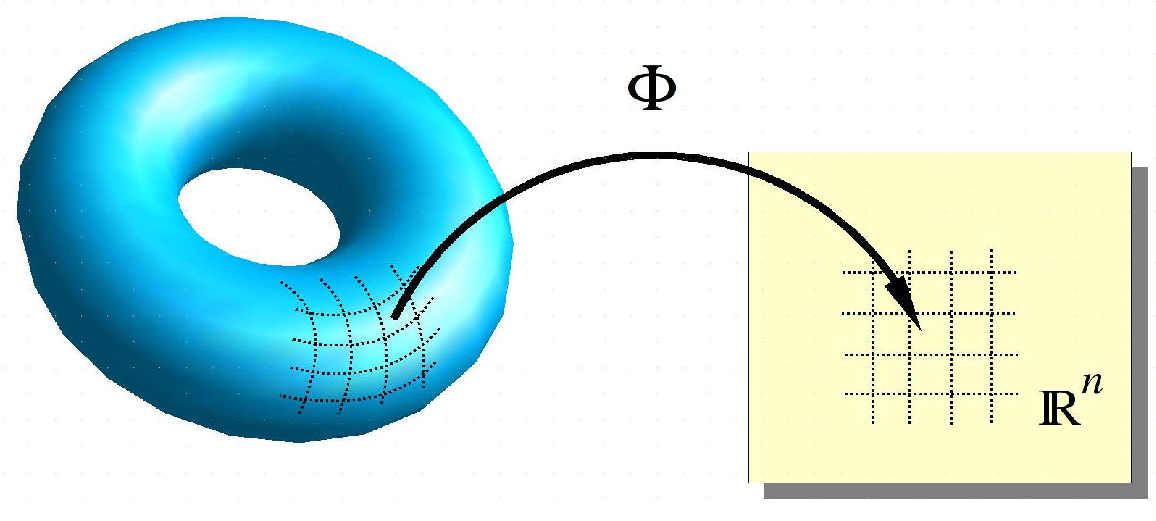
\includegraphics[width=0.8\textwidth]{bas_manifold.pdf}}
\caption[]{\label{f:bas:manifold} \footnotesize
Locally a manifold resembles $\R^n$ ($n=2$ on the figure), but this is not necessarily the case at the global level.}
\end{figure}

\begin{remark}
In relativity, it is customary to label the $n$ coordinates by an index
ranging from $0$ to $n-1$. Actually, this convention is mostly used when $\M$ is the spacetime manifold ($n=4$ in standard general relativity). The computer-oriented reader will have noticed the similarity
with the index ranging of arrays in the C/C++ or Python programming languages.
\end{remark}


\begin{remark} \label{r:bas:topol_manif}
Strictly speaking the definition given above is that of a \defin{topological manifold}\index{topological manifold}\index{manifold!topological}. We are saying \emph{manifold} for short.
\end{remark}


Usually, one needs more than one coordinate system to cover $\M$.
An \defin{atlas}\index{atlas} on $\M$ is a finite set of pairs
$(\mathcal{U}_k,\Phi_k)_{1\leq k \leq K}$,  where $K$ is a non-zero integer, $\mathcal{U}_k$ an open set of $\M$ and $\Phi_k$ a chart on $\mathcal{U}_k$,
such that the union of all $\mathcal{U}_k$ covers $\M$:
\be
	\bigcup_{k=1}^K \mathcal{U}_k = \M.
\ee

The above definition of a manifold lies at the \emph{topological} level
(cf.~Remark~\ref{r:bas:topol_manif}), meaning that one has the notion of continuity, but not of differentiability. To get the latter, one should rely on the smooth structure of $\R^n$, via the atlases:
a \defin{smooth manifold}\index{smooth!manifold}\index{manifold!smooth --},
is a manifold $\M$ equipped with an atlas
$(\mathcal{U}_k,\Phi_k)_{1\leq k \leq K}$ such that for any non-empty intersection
$\mathcal{U}_i \cap \mathcal{U}_j$, the mapping
\be \label{e:bas:transition_map}
	\Phi_i \circ \Phi_j^{-1} : \Phi_j(\mathcal{U}_i \cap \mathcal{U}_j)
	\subset \R^n \longrightarrow \Phi_i(\mathcal{U}_i \cap \mathcal{U}_j)
	\subset \R^n
\ee
is smooth (i.e. $C^\infty$).
Note that the above mapping is from an open set of $\R^n$ to an open set of $\R^n$, so that the invoked differentiability is nothing but that of $\R^n$.
The atlas $(\mathcal{U}_k,\Phi_k)_{1\leq k \leq K}$ is called a
\defin{smooth atlas}\index{smooth!atlas}\index{atlas!smooth --}.
In the following, we consider only smooth manifolds.

Given two smooth manifolds, $\M$ and $\M'$, of
respective dimensions $n$ and $n'$, we say that a map
$\phi : \M \rightarrow \M'$ is \defin{smooth map}\index{smooth!map} iff in some (and hence all, thanks to the smoothness of (\ref{e:bas:transition_map})) coordinate systems
of $\M$ and $\M'$ belonging to the smooth atlases of $\M$ and $\M'$,
the coordinates of the image $\phi(p)$ are smooth functions $\R^n\rightarrow \R^{n'}$ of the coordinates of $p$.
The map $\phi$ is said to be a \defin{diffeomorphism}\index{diffeomorphism} iff
it is bijective and both $\phi$ and $\phi^{-1}$ are smooth. This implies $n=n'$.

\begin{remark}
Strictly speaking a smooth manifold is a pair $(\M,\mathcal{A})$  where
$\mathcal{A}$ is a (maximal) smooth atlas on $\M$.
Indeed a given (topological) manifold $\M$
can have non-equivalent differentiable structures, as shown by Milnor (1956) \cite{Milno56}
in the specific case of the unit sphere of dimension~7, $\mathbb{S}^7$: there exist smooth manifolds, the so-called \emph{exotic spheres}\index{exotic!sphere},
that are homeomorphic to $\mathbb{S}^7$ but not diffeomorphic
to $\mathbb{S}^7$.  On the other side, for $n\leq 6$, there is a unique smooth
structure for the sphere $\mathbb{S}^n$.
Moreover, any manifold of dimension $n\leq 3$ admits a unique smooth structure.
Amazingly, in the case of $\R^n$, there exists a unique smooth structure (the standard one) for any $n\not=4$, but for $n=4$ (the spacetime case !) there exist uncountably many non-equivalent smooth structures, the so-called
\emph{exotic $\R^4$}\index{exotic!$\R^4$} \cite{Taube87}.
\end{remark}

\subsection{Vectors on a manifold} \label{s:bas:vectors}

On a manifold, vectors are defined as tangent vectors to a curve.
A \defin{curve}\index{curve} is a subset $\mathcal{C}\subset \M$ which is the image of a smooth function $\R  \rightarrow  \M$:
\be
	\begin{array}{rccl}
	P: & \R & \longrightarrow & \M \\
		& \lambda & \longmapsto & p = P(\lambda) \in \mathcal{C}.
	\end{array}
\ee
Hence $\mathcal{C} = \{ P(\lambda) |\ \lambda\in\R\}$. The function $P$ is called a
\defin{parametrization}\index{parametrization} of $\mathcal{C}$ and the
variable $\lambda$ is called a \defin{parameter along $\mathcal{C}$}\index{parameter along a curve}. Given a coordinate system $(x^\alpha)$
in a neighbourhood of a point $p\in\mathcal{C}$, the parametrization $P$ is
defined by $n$ functions $X^\alpha : \ \R\rightarrow \R$ such that
\be
  x^\alpha(P(\lambda)) = X^\alpha(\lambda) .
\ee

A \defin{scalar field}\index{scalar!field} on $\M$ is a function
$f:\ \M \rightarrow \R$. In practice, we will always consider smooth scalar fields. At a point $p=P(\lambda)\in\mathcal{C}$, the \defin{vector tangent to $\mathcal{C}$}\index{vector!tangent to a curve}\index{tangent!vector} associated with the parametrization
$P$ is the operator $\w{v}$ which maps every scalar field $f$ to the real number
\be \label{e:bas:def_vector}
  \w{v}(f) = \left. \frac{\D f}{\D \lambda} \right|_{\mathcal{C}} :=
  \lim_{\varepsilon\rightarrow 0} \frac{1}{\varepsilon}
  \left[ f(P(\lambda+\varepsilon)) - f(P(\lambda)) \right] .
\ee
Given a coordinate system $(x^\alpha)$ around some point $p\in\M$, there are
$n$ curves $\mathcal{C}_\alpha$ through $p$ associated with $(x^\alpha)$ and called the
\defin{coordinate lines}\index{coordinate!line}\index{line!coordinate}:
for each $\alpha\in\{0,\ldots,n-1\}$, $\mathcal{C}_\alpha$ is defined as the curve through $p$ parametrized by $\lambda = x^\alpha$ and having constant coordinates
$x^\beta$ for all $\beta\not=\alpha$.
The vector tangent to $\mathcal{C}_\alpha$ parametrized by $x^\alpha$ is
denoted $\wpar_\alpha$. Its action on a scalar field $f$ is by definition
\[
  \wpar_\alpha(f) =
  \left. \frac{\D f}{\D x^\alpha} \right|_{\mathcal{C}_\alpha}
  = \left. \frac{\D f}{\D x^\alpha} \right|_{x^\beta={\rm const}\atop \beta\not=\alpha} .
\]
Considering $f$ as a function of
the coordinates $(x^0,\ldots,x^{n-1})$ (whereas strictly speaking it is a function
of the points on $\M$) we recognize in the last term the partial derivative of
$f$ with respect to $x^\alpha$. Hence
\be \label{e:bas:wpar_partial}
 \encadre{ \wpar_\alpha(f) = \der{f}{x^\alpha} } .
\ee
Similarly, we may rewrite (\ref{e:bas:def_vector}) as
\bea
  \w{v}(f) & = & \lim_{\varepsilon\rightarrow 0} \frac{1}{\varepsilon}
  \left[ f(X^0(\lambda+\varepsilon),\ldots,X^{n-1}(\lambda+\varepsilon))
  - f(X^0(\lambda),\ldots,X^{n-1}(\lambda)) \right] \nonumber \\
  & = & \der{f}{x^\alpha} \frac{\D X^\alpha}{\D \lambda}
  = \wpar_\alpha(f) \frac{\D X^\alpha}{\D \lambda} . \nonumber
\eea
In the above equation and throughout the all book,
we are using \defin{Einstein summation convention}\index{Einstein!summation convention}: a repeated index implies a summation over all the possible values of this index
(here from $\alpha=0$ to $\alpha=n-1$).
The above identity being valid for any scalar field $f$, we conclude that
\be \label{e:bas:v_va_wpar_a}
  \encadre{ \w{v} = v^\alpha \, \wpar_\alpha } ,
\ee
with the $n$ real numbers
\be
  v^\alpha := \frac{\D X^\alpha}{\D \lambda} , \qquad 0 \leq \alpha\leq n-1 .
\ee
Since every vector tangent to a curve at $p$ is expressible as (\ref{e:bas:v_va_wpar_a}), we conclude that
the set of all vectors tangent to a curve at $p$ is a vector space of dimension $n$ and that $(\wpar_\alpha)$ constitutes a basis of it. This vector space is
called the
\defin{tangent vector space to $\M$ at $p$}\index{tangent!vector space}\index{vector!space tangent to a manifold} and is denoted $T_p\M$.
The elements of $T_p\M$ are simply called \defin{vectors}\index{vector} at $p$.
The basis $(\wpar_\alpha)$ is called the \defin{natural basis}\index{natural basis}\index{basis!natural} associated with
the coordinates $(x^\alpha)$ and the coefficients $v^\alpha$ in (\ref{e:bas:v_va_wpar_a}) are called the \defin{components of the vector $\w{v}$ with respect to the coordinates $(x^\alpha)$}\index{component!w.r.t. a coordinate system}.
The tangent vector space is represented at two different points in Fig.~\ref{f:bas:tang_space}.

\begin{figure}
\centerline{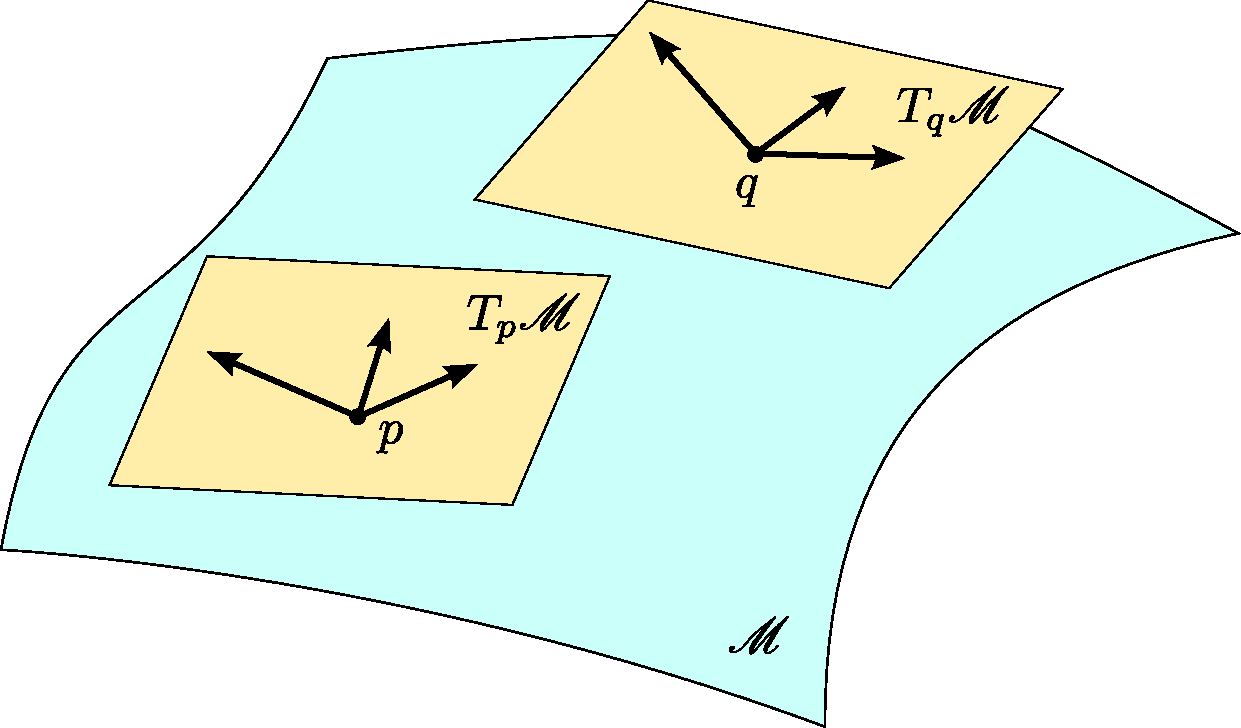
\includegraphics[width=0.8\textwidth]{bas_tang_space.pdf}}
\caption[]{\label{f:bas:tang_space} \footnotesize
The vectors at two points $p$ and $q$ on the
manifold $\M$ belong to two different vector spaces:
the tangent spaces $T_p\M$ and $T_q\M$.}
\end{figure}

Contrary to what happens for an affine space, one cannot, in general, define a vector connecting two points $p$ and $q$ on a manifold, except if $p$ and $q$ are infinitesimally close to each other. Indeed, in the latter case, we may define
the \defin{infinitesimal displacement vector from $p$ to $q$}\index{infinitesimal! displacement vector}\index{vector!infinitesimal --} as the vector $\D\w{x}\in{{T_p\M}}$ whose action on a scalar field $f$ is
\be \label{e:bas:dell_f}
  \D\w{x}(f) = \left. \D f \right| _{p\rightarrow q} = f(q) - f(p) .
\ee
Since $p$ and $q$ are infinitesimally close, there is a unique (piece of) curve
$\mathcal{C}$ going
from $p$ to $q$ and one has
\be \label{e:bas:dell_v_dlamb}
  \D\w{x} = \w{v} \, \D\lambda ,
\ee
where $\lambda$ is a parameter along $\mathcal{C}$, $\w{v}$ the associated tangent
vector at $p$ and $\D\lambda$ the parameter
increment from $p$ to $q$: $p=P(\lambda)$ and $q=P(\lambda+\D\lambda)$.
The relation (\ref{e:bas:dell_v_dlamb}) follows immediately from the definition
(\ref{e:bas:def_vector}) of $\w{v}$.
Given a coordinate system, let $(x^\alpha)$ be the coordinates
of $p$ and $(x^\alpha+\D x^\alpha)$ those of $q$. Then from Eq.~(\ref{e:bas:dell_f}),
\[
  \D\w{x}(f) =   \D f  = \der{f}{x^\alpha} \, \D x^\alpha
  = \D x^\alpha \, \wpar_\alpha(f) .
\]
The scalar field $f$ being arbitrary, we conclude that
\be \label{e:bas:dell_dxa_wpar}
  \encadre{ \D\w{x} = \D x^\alpha \, \wpar_\alpha } .
\ee
In other words, the components of the infinitesimal displacement vector with respect
to the coordinates $(x^\alpha)$ are nothing but the infinitesimal coordinate
increments $\D x^\alpha$.

\subsection{Linear forms} \label{s:bas:linear_form}

A fundamental operation on vectors consists in mapping them to real numbers, and this in a linear way. More precisely, at each point $p\in\M$, one defines a \defin{linear form}\index{linear form}\index{form!linear}
as a mapping\footnote{We are using the same bra-ket notation as in quantum mechanics to denote the action of a linear form on a vector.}
\be \label{e:bas:def_lin_form}
	\begin{array}{rccl}
	\w{\omega}: & T_p\M & \longrightarrow & \R \\
		& \w{v} & \longmapsto & \langle \w{\omega}, \w{v} \rangle
	\end{array}
\ee
that is linear:
$\langle\w{\omega},\lambda \w{v} + \w{u}\rangle =  \lambda \langle\w{\omega},\w{v}\rangle +  \langle\w{\omega},\w{u}\rangle$ for all $\w{u},\w{v}\in{T_p\M}$ and $\lambda\in\R$. The set of all linear forms at $p$ constitutes a $n$-dimensional vector
space, which is called the \defin{dual space of $T_p\M$}\index{dual!vector space} and denoted by ${T_p^*\M}$.
Given the natural basis $(\wpar_\alpha)$ of $T_p\M$ associated with some coordinates
$(x^\alpha)$, there is a unique basis of ${T_p^*\M}$, denoted by $(\dd x^\alpha)$, such that
\be \label{e:bas:dual_basis_nat}
  \encadre{ \langle \dd x^\alpha ,\wpar_\beta\rangle = \delta^\alpha_{\ \  \beta} } ,
\ee
where $\delta^\alpha_{\ \ \beta}$ is the \defin{Kronecker symbol}\index{Kronecker symbol} :
$\delta^\alpha_{\ \  \beta} = 1$ if $\alpha=\beta$ and $0$ otherwise.
The basis $(\dd x^\alpha)$ is called the \defin{dual basis}\index{dual!basis}\index{basis!dual} of the basis
$(\wpar_\alpha)$. The notation $(\dd x^\alpha)$ stems from the fact that if we apply
the linear form $\dd x^\alpha$ to the infinitesimal displacement vector
(\ref{e:bas:dell_dxa_wpar}), we get nothing but the number $\D x^\alpha$:
\be \label{e:bas:dxa_dxa}
    \langle\dd x^\alpha,\D\w{x} \rangle = \langle\dd x^\alpha , \D x^\beta \, \wpar_\beta
    \rangle
    = \D x^\beta \underbrace{\langle \dd x^\alpha , \wpar_\beta \rangle}_{\delta^\alpha_{\ \ \beta}}
    = \D x^\alpha .
\ee
\begin{remark}
Do not confuse the linear form $\dd x^\alpha$ with the infinitesimal increment
$\D x^\alpha$ of the coordinate $x^\alpha$.
\end{remark}

The dual basis can be used to expand any linear form $\w{\omega}$, thereby defining its
\defin{components $\omega_\alpha$ with respect to the coordinates $(x^\alpha)$}\index{component!of a linear form}:
\be \label{e:bas:def_comp_form}
  \w{\omega} = \omega_\alpha \, \dd x^\alpha .
\ee
In terms of components, the action of a linear form on a vector takes then a very simple form:
\be
  \encadre{ \langle\w{\omega},\w{v}\rangle  = \omega_\alpha v^\alpha }.
\ee
This follows immediately from (\ref{e:bas:def_comp_form}),
(\ref{e:bas:v_va_wpar_a}) and (\ref{e:bas:dual_basis_nat}).

A field of linear forms, i.e. a (smooth) map which associates to each point $p\in\M$ a member of $T_p\M$ is called a \defin{1-form}\index{1-form}.
Given a smooth scalar field $f$ on $\M$, there exists a 1-form canonically associated with it, called
the \defin{differential of $f$}\index{differential} and denoted $\wnab f$.
At each point $p\in\M$, $\wnab f$ is the unique linear form which, once
applied to the infinitesimal displacement vector $\D\w{x}$ from $p$ to a
nearby point $q$, gives the change in $f$ between points $p$ and $q$:
\be \label{e:bas:df}
  \D f := f(q) - f(p) = \langle \wnab f, \D\w{x} \rangle .
\ee
Since $\D f = \dert{f}{x^\alpha} \, \D x^\alpha$, Eq.~(\ref{e:bas:dxa_dxa}) implies that the components of the differential with respect to the dual basis are nothing but the partial derivatives of $f$ with respect to the coordinates $(x^\alpha)$ :
\be \label{e:bas:grad_f_der_f}
  \encadre{ \wnab f = \der{f}{x^\alpha} \, \dd x^\alpha } .
\ee

\begin{remark}
In non-relativistic physics, the concept of \defin{gradient}\index{gradient}
of a scalar field is commonly used instead of the
differential, the former being a vector field and the latter a 1-form.
This is so because one associates implicitly a vector
$\vw{\omega}$ to any 1-form $\w{\omega}$ via the Euclidean scalar product
of $\R^3$: $\forall \overrightarrow{v}\in \R^3,\ \langle \w{\omega},\overrightarrow{v}\rangle = \vw{\omega}\cdot\overrightarrow{v}$.
Accordingly, formula (\ref{e:bas:df}) is rewritten as
$\D f = \vw{\nabla} f \cdot \D\w{x}$. But we should keep in mind
that, at the fundamental level, the key quantity is the differential 1-form
$\wnab f$, for Eq.~(\ref{e:bas:df}) does not require any metric on the
manifold $\M$ to be
meaningful. The gradient $\vw{\nabla} f$ is a derived quantity, obtained
from the differential $\wnab f$ by metric duality.
\end{remark}

\begin{remark}
For a fixed value of $\alpha$, the coordinate $x^\alpha$ can be considered as a scalar field on $\M$.
If we apply (\ref{e:bas:grad_f_der_f}) to $f=x^\alpha$, we then get
\be \label{e:bas:nab_xa_dxa}
  \wnab x^\alpha = \dd x^\alpha .
\ee
Hence the dual basis to the natural basis $(\wpar_\alpha)$ is formed by the
differentials of the coordinates.
\end{remark}

Of course the natural bases are not the only possible bases in the vector
space $T_p\M$. One may use a basis $(\w{e}_\alpha)$ that is not related to a coordinate system on $\M$, for instance an orthonormal basis with respect to some metric.
There exists then a unique basis $(\w{e}^\alpha)$
of the dual space ${T_p^*\M}$ such that\footnote{Notice that,
according to the standard usage, the symbol for the vector $\w{e}_\alpha$ and that for the linear form $\w{e}^\alpha$ differ only by the position of the index $\alpha$.}
\be \label{e:bas:dual_basis}
  \encadre{ \langle \w{e}^\alpha , \w{e}_\beta \rangle = \delta^\alpha_{\ \ \beta} } .
\ee
$(\w{e}^\alpha)$ is called the \defin{dual basis}\index{dual!basis}\index{basis!dual} to
$(\w{e}_\alpha)$.
The relation (\ref{e:bas:dual_basis_nat}) is a special case
of (\ref{e:bas:dual_basis}), for which $\w{e}_\alpha = \wpar_\alpha$ and $\w{e}^\alpha = \dd x^\alpha$.


\subsection{Tensors} \label{s:bas:tensors}

Tensors are generalizations of both vectors and linear forms.
At a point $p\in\M$,
a \defin{tensor of type}\index{tensor} $(k,\ell)$ with $(k,\ell)\in\mathbb{N}^2$, also called \defin{tensor $k$ times
contravariant and $\ell$ times covariant}\index{contravariant}\index{covariant}\index{type of a tensor}, is a
mapping
\be \label{e:bas:def_tensor}
	\begin{array}{rccc}
	\w{T}: & \underbrace{{T_p^*\M}\times\cdots\times{T_p^*\M}}_{k {\ \rm times}}
	\times \underbrace{T_p\M\times\cdots\times{T_p\M}}_{\ell {\ \rm times}} &
	 \longrightarrow & \R  \\
	& (\w{\omega}_1,\ldots,\w{\omega}_k,\w{v}_1,\ldots,\w{v}_\ell) &
		 \longmapsto &
	\w{T}(\w{\omega}_1,\ldots,\w{\omega}_k, \w{v}_1,\ldots,\w{v}_\ell)
	\end{array}
\ee
that is linear with respect to each of its arguments. The integer $k+\ell$ is
called the tensor \defin{valence}\index{valence}, or sometimes the
tensor \defin{rank}\index{rank of a tensor} or \defin{order}\index{order of a tensor}. Let us recall the canonical duality
$T_p^{**}\M={T_p\M}$, which means that every vector $\w{v}$ can be considered
as a linear form on the space ${T_p^*\M}$, via
${T_p^*\M}\rightarrow \R$,
$\w{\omega}\mapsto \langle \w{\omega},\w{v}\rangle$.
Accordingly a vector is a tensor of type $(1,0)$. A linear form is a
tensor of type $(0,1)$. A tensor of type $(0,2)$ is called a
\defin{bilinear form}\index{bilinear form}\index{form!bilinear}. It maps pairs of vectors to real numbers, in a linear way for each
vector.

Given a basis $(\w{e}_\alpha)$ of $T_p\M$
and the corresponding dual basis $(\w{e}^\alpha)$ in ${T_p^*\M}$, we
can expand any tensor $\w{T}$ of type $(k,\ell)$ as
\be \label{e:bas:def_components}
	\encadre{\w{T} = T^{\alpha_1\ldots\alpha_k}_{\qquad\ \; \beta_1\ldots\beta_\ell}
		\; \w{e}_{\alpha_1} \otimes \ldots \otimes \w{e}_{\alpha_k}
                \otimes
		\w{e}^{\beta_1} \otimes \ldots \otimes \w{e}^{\beta_\ell} } ,
\ee
where the \defin{tensor product}\index{tensor!product}\index{product!tensor} $ \w{e}_{\alpha_1} \otimes \ldots \otimes \w{e}_{\alpha_k} \otimes
\w{e}^{\beta_1} \otimes \ldots \otimes \w{e}^{\beta_\ell}$ is the tensor of
type $(k,\ell)$ for which the image of  $(\w{\omega}_1,\ldots,\w{\omega}_k,\w{v}_1,\ldots,\w{v}_\ell)$ as in
(\ref{e:bas:def_tensor}) is the real number
\[
	\prod_{i=1}^k \langle \w{\omega}_i,\w{e}_{\alpha_i}\rangle \;\times\;
	\prod_{j=1}^\ell \langle \w{e}^{\beta_j},\w{v}_j\rangle .
\]
Notice that all the products in the above formula are simply products in $\R$.
The $n^{k+\ell}$ scalar coefficients  $T^{\alpha_1\ldots\alpha_k}_{\qquad\ \; \beta_1\ldots\beta_\ell}$ in (\ref{e:bas:def_components}) are called the \defin{components
of the tensor $\w{T}$ with respect to the basis $(\w{e}_\alpha)$}\index{component!of a tensor}.
These components are unique and fully characterize
the tensor $\w{T}$.

\begin{remark}
The notations $v^\alpha$ and $\omega_\alpha$ already introduced for the components
of a vector $\w{v}$ [Eq.~(\ref{e:bas:v_va_wpar_a})]
or a linear form $\w{\omega}$ [Eq.~(\ref{e:bas:def_comp_form})] are of course the
particular cases $(k,\ell)=(1,0)$ or $(k,\ell)=(0,1)$ of (\ref{e:bas:def_components}), with,
in addition, $\w{e}_\alpha=\wpar_\alpha$ and $\w{e}^\alpha = \dd x^\alpha$.
\end{remark}


\subsection{Fields on a manifold} \label{s:bas:fields}

A \defin{tensor field}\index{tensor!field}\index{field!tensor} of type $(k,\ell)$ is a map
which associates to each point $p\in\M$ a tensor of type $(k,\ell)$ on $T_p\M$.
By convention, a scalar field\index{scalar!field}\index{field!scalar} is considered as a tensor field of type $(0,0)$.
We shall consider only smooth fields.

Given a non-negative integer $p$, a
\defin{differential form of order $p$}\index{form!differential}\index{differential!form},
or
\defin{$p$-form}\index{$p$-form}\index{form!$p$-form}, is a tensor field of type $(0,p)$, i.e.
a field of $p$-linear forms, that is fully antisymmetric whenever $p\geq 2$.
This definition generalizes that of a 1-form given in Sec.~\ref{s:bas:linear_form}.

A \defin{frame field}\index{frame field} or
\defin{moving frame}\index{moving!frame} is a $n$-uplet of vector fields
$(\w{e}_\alpha)$ such that at each point $p\in\M$, $(\w{e}_\alpha(p))$ is
a basis of the tangent space $T_p\M$.
If $n=4$, a frame field is also called a \defin{tetrad}\index{tetrad} and if $n=3$,
it is called a
\defin{triad}\index{triad}.

Given a vector field $\w{v}$ and a scalar field $f$, the function
$\M\rightarrow \R$, $p\mapsto \left.\w{v}\right|_p(f)$ clearly defines a scalar field on
$\M$, which we denote naturally by $\w{v}(f)$.
We may then define the \defin{commutator of two vector fields}\index{commutator} $\w{u}$
and $\w{v}$ as the vector field $[\w{u},\w{v}]$ whose action on a scalar field $f$ is
\be
  [\w{u},\w{v}](f) := \w{u}(\w{v}(f)) - \w{v}(\w{u}(f)) .
\ee
With respect to a coordinate system $(x^\alpha)$, it is not difficult, via
(\ref{e:bas:v_va_wpar_a}), to see that the components of the commutator are
\be \label{e:bas:commut_comp}
  \encadre{ [\w{u},\w{v}]^\alpha = u^\mu \der{v^\alpha}{x^\mu}
    - v^\mu \der{u^\alpha}{x^\mu} } .
\ee

\subsection{Immersions, embeddings and submanifolds} \label{s:bas:embed}

Let $\M$ and $\mathscr{N}$ be two smooth manifolds
and
\be
    \Phi:\ \M \longrightarrow \mathscr{N}
\ee
be a smooth map (cf. Sec.~\ref{s:bas:def_manif}).
At a given point $p\in\M$, the \defin{differential}\index{differential!of a smooth map}
of $\Phi$ is the linear map
\be
    \left.\D\Phi \right| _p:\ T_p\M \longrightarrow T_{\Phi(p)}\mathscr{N}
\ee
that ``approximates'' $\Phi$ in the following sense: if $\D\w{x}\in T_p\M$ is the
infinitesimal displacement vector from $p$ to some (infinitesimally close) point $q$,
then
\be \label{e:bas:def_diff_map}
    \left.\D\Phi \right| _p(\D\w{x}) = \D\w{L},
\ee
where $\D\w{L}$ is the infinitesimal displacement vector of $T_{\Phi(p)}\mathscr{N}$
connecting $\Phi(p)$ to $\Phi(q)$ (cf. Fig.~??).
In terms of the characterization of vectors by their action on scalar fields
[Eq.~(\ref{e:bas:def_vector})], it is easy to see, thanks to (\ref{e:bas:dell_f}),
that the definition (\ref{e:bas:def_diff_map}) is equivalent to
\be
    \forall \w{v}\in T_p\M,\ \forall f \in C^\infty(\mathscr{N},\mathbb{R}),\quad
    \left.\D\Phi \right| _p(\w{v})(f) =
        \w{v}\left(f\circ \Phi \right) .
\ee

The smooth map $\Phi$ is called an \defin{immersion}\index{immersion} iff
the differential $\left.\D\Phi \right| _p$ is injective at any point $p\in\M$.
Moreover $\Phi$ is called an \defin{embedding}\index{embedding} iff (i) $\Phi$
is an immersion and (ii) $\Phi$ is a homeomorphism $\M \rightarrow \Phi(\M)$.
Note that an embedding is necessarily injective, contrary to an immersion.

A \defin{submanifold} of $\M$ is a subset $\mathscr{S}\subset \M$ such
that (i) $\mathscr{S}$ is a manifold in the subspace topology and (ii)
$\mathscr{S}$ has a smooth structure with respect to which
the inclusion map $\iota: \mathscr{S} \rightarrow \M$ is an embedding.
One can show that $\mathscr{S}$ is a submanifold of $\M$ iff there exists
a manifold $\mathscr{S}_0$ (a priori not included in $\M$) and an
embedding $\Phi: \mathscr{S}_0 \rightarrow \M$, such that
$\mathscr{S} = \Phi(\mathscr{S}_0)$.

\begin{remark}
Scritly speaking, the above definition regards an
\defin{embedded submanifold}\index{embedded!submanifold}\index{submanifold!embedded --};
there is also the wider concept of \defin{immersed submanifold}\index{immersed!submanifold}\index{submanifold!immersed --} (see e.g. Chap~5 of \cite{Lee13}).
\end{remark}


One has necessarily $\dim \mathscr{S} \leq \dim \M$. The non-negative integer
$m = \dim\M - \dim\mathscr{S}$ is called the \defin{codimension}\index{codimension}
of the submanifold $\mathscr{S}$. A submanifold of codimension 1 is called
a \defin{hypersurface}\index{hypersurface}. A submanifold of dimension 1 is
(the image of) a curve in $\M$, but note that not all curves are submanifolds:
a curve with self-crossing points is not a submanifold.





%%%%%%%%%%%%%%%%%%%%%%%%%%%%%%%%%%%%%%%%%%%%%%%%%%%%%%%%%%%%%%%%%%%%%%%%%%%%%%%

\section{Pseudo-Riemannian manifolds} \label{s:bas:pRiemManif}

\subsection{Metric tensor} \label{s:bas:metric}

A \defin{pseudo-Riemannian manifold}\index{pseudo-Riemannian manifold}\index{manifold!pseudo-Riemannian} is a pair $(\M,\w{g})$ where $\M$ is a smooth manifold
and $\w{g}$ is a \defin{metric tensor}\index{metric!tensor}\index{metric} on $\M$,
i.e. a tensor field obeying the following properties:
\begin{enumerate}
\item $\w{g}$ is a tensor field of type $(0,2)$: at each point $p\in\M$, $\w{g}(p)$ is a
bilinear form acting on vectors in the tangent space $T_p\M$:
\be
	\begin{array}{rccl}
	\w{g}(p): & {T_p\M}\times{T_p\M} & \longrightarrow & \R \\
		& (\w{u},\w{v}) & \longmapsto & \w{g}(\w{u},\w{v}) .
	\end{array}
\ee
\item $\w{g}$ is \defin{symmetric}\index{symmetric}: $\w{g}(\w{u},\w{v}) = \w{g}(\w{v},\w{u})$.
\item $\w{g}$ is \defin{non-degenerate}\index{non-degenerate!bilinear form}: at any point
$p\in\M$,
a vector $\w{u}$ such that
$\forall \w{v}\in{T_p\M},\ \w{g}(\w{u},\w{v}) = 0$ is necessarily the null vector.
\end{enumerate}
The properties of being symmetric and non-degenerate are typical of a
\defin{scalar pro\-duct}\index{scalar!product}. Accordingly,
one says that two vectors
$\w{u}$ and $\w{v}$ are \defin{$\w{g}$-orthogonal}\index{g-orthogonal} (or simply \defin{orthogonal}\index{orthogonal} if there is no ambiguity) iff $\w{g}(\w{u},\w{v}) = 0$.
Moreover, when there is no ambiguity on the metric (usually the spacetime metric), we are
using a dot to denote the scalar product of two vectors taken with $\w{g}$:
\be
  \forall (\w{u},\w{v})\in{T_p\M}\times{T_p\M},\quad
  \encadre{ \w{u}\cdot\w{v} = \w{g}(\w{u},\w{v}) } .
\ee

In a given basis $(\w{e}_\alpha)$ of $T_p\M$, the components of $\w{g}$
is the matrix $(g_{\alpha\beta})$ defined by
formula (\ref{e:bas:def_components}) with $(k,\ell)=(0,2)$:
\be
  \w{g} = g_{\alpha\beta} \, \w{e}^\alpha \otimes \w{e}^\beta .
\ee
For any pair $(\w{u},\w{v})$ of vectors we have then
\be
  \w{g}(\w{u},\w{v}) = g_{\alpha\beta} u^\alpha v^\beta .
\ee
In particular, considering the natural basis associated with some coordinate system
$(x^\alpha)$, the scalar square of an infinitesimal displacement vector $\D\w{x}$
[cf. Eq.~(\ref{e:bas:dell_f})] is
\be
  \D s^2 := \w{g}(\D\w{x},\D\w{x}) = g_{\alpha\beta} \D x^\alpha \, \D x^\beta .
\ee
This formula, which follows from the value (\ref{e:bas:dell_dxa_wpar}) of the
components of $\D\w{x}$, is called the expression of the \defin{line element}\index{line!element}
on the pseudo-Riemannian manifold $(\M,\w{g})$. It is often used to define the metric tensor in
general relativity texts. Note that contrary to what the notation may suggest, $\D s^2$ is not necessarily a positive quantity.

\subsection{Signature and orthonormal bases} \label{s:bas:signature}

An important feature of the metric tensor is its \defin{signature}\index{signature}:
in all bases of $T_p\M$ where the components $(g_{\alpha\beta})$ form a diagonal matrix, there is necessarily the same number, $s$ say, of negative components
and the same number, $n-s$, of positive components. The independence of $s$ from the choice
of the basis where $(g_{\alpha\beta})$ is diagonal is a basic result of linear algebra named \defin{Sylvester's law of inertia}\index{Sylvester's law of inertia}. One writes:
\be
  \mathrm{sign}\; \w{g} = (\underbrace{-,\ldots,-}_{\mbox{$s$ times}},
  \underbrace{+,\ldots,+}_{\mbox{$n-s$ times}}) .
\ee

If $s=0$, $\w{g}$ is called a \defin{Riemannian metric}\index{Riemannian!metric} and
$(\M,\w{g})$ a \defin{Riemannian manifold}\index{Riemannian!manifold}. In this case, $\w{g}$ is
\defin{positive-definite}, which means that
\be
  \forall \w{v}\in{T_p\M},\quad \w{g}(\w{v},\w{v}) \geq 0
\ee
and $\w{g}(\w{v},\w{v}) = 0$ iff $\w{v}=0$.
A standard example of Riemannian metric is of course the scalar product of the Euclidean space
$\R^n$.

If $s=1$, $\w{g}$ is called a \defin{Lorentzian metric}\index{Lorentzian!metric} and
$(\M,\w{g})$ a \defin{Lorentzian manifold}\index{Lorentzian!manifold}. One may then have
$\w{g}(\w{v},\w{v}) < 0$; vectors for which this occurs are called \defin{timelike}\index{timelike!vector},
whereas vectors for which $\w{g}(\w{v},\w{v}) > 0$ are called \defin{spacelike}\index{spacelike!vector},
and those for which $\w{g}(\w{v},\w{v}) = 0$ are called \defin{null}\index{null!vector}. The subset of $T_p\M$ formed by all null
vectors is termed the \defin{null cone}\index{null!cone} of $\w{g}$ at $p$.

A basis $(\w{e}_\alpha)$ of $T_p\M$ is called a \defin{$\w{g}$-orthonormal basis}\index{g-orthonormal basis} (or simply \defin{orthonormal basis}\index{orthonormal basis} if there
is no ambiguity on the metric) iff\footnote{No summation on $\alpha$ is implied.}
\be
   \begin{array}{lcll}
  \w{g}(\w{e}_\alpha,\w{e}_\alpha) = -1 &\quad \mbox{for}\quad & 0 \leq \alpha \leq s-1 \\
  \w{g}(\w{e}_\alpha,\w{e}_\alpha) = 1 & \quad \mbox{for}\quad &s \leq \alpha \leq n-1 \\
  \w{g}(\w{e}_\alpha,\w{e}_\beta)  = 0 & \quad \mbox{for}\quad & \alpha\not=\beta .
  \end{array}
\ee

\subsection{Metric duality} \label{s:bas:metric_dual}

Since the bilinear form $\w{g}$ is non-degenerate, its matrix $(g_{\alpha\beta})$ in
any basis $(\w{e}_\alpha)$ is invertible and the inverse\index{inverse!metric} is denoted by $(g^{\alpha\beta})$:
\be
  \encadre{ g^{\alpha\mu} g_{\mu\beta} = \delta^\alpha_{\ \ \beta} }.
\ee
The metric $\w{g}$ induces an isomorphism between
$T_p\M$ (vectors) and ${T_p^*\M}$ (linear forms) which, in  index notation,
corresponds to the lowering\index{lowering an index}\index{index!lowering} or
raising of the index\index{raising an index}\index{index!raising} by contraction
with $g_{\alpha\beta}$ or $g^{\alpha\beta}$.
In the present book, an index-free symbol will always denote
a tensor with a fixed covariance type (such as a vector, a 1-form,
a bilinear form, etc.). We will therefore use a different symbol
to denote its image under the metric isomorphism.
In particular, we denote by an underbar the
isomorphism $T_p\M \rightarrow {T_p^*\M}$
and by an arrow the reverse isomorphism ${T_p^*\M} \rightarrow T_p\M$:
\begin{enumerate}
\item For any vector $\w{u}$ in $T_p\M$, $\uu{u}$ stands for
the unique linear form such that
\be \label{e:bas:underbar}
	\forall \w{v} \in T_p\M,\quad \langle \uu{u}, \w{v}
		\rangle = \w{g}(\w{u},\w{v}) .
\ee
However, we will omit the underbar on the components
of $\uu{u}$, since
the position of the index allows us to distinguish between vectors
and  linear forms, following the standard usage:
if the components of
$\w{u}$ in a given basis $(\w{e}_\alpha)$ are denoted by $u^\alpha$,
the components of $\uu{u}$ in the dual basis $(\w{e}^\alpha)$
are then denoted by $u_\alpha$ and are given by
\be
  u_\alpha = g_{\alpha\mu} u^\mu .
\ee
\item For any linear form $\w{\omega}$ in ${T_p^*\M}$, $\vw{\w{\omega}}$
stands for the unique vector of $T_p\M$ such that
\be \label{e:bas:arrow_form}
	\forall \w{v} \in T_p\M,\quad
        \w{g}(\vw{\w{\omega}},\w{v}) =
        \langle \w{\omega}, \w{v} \rangle .
\ee
As for the underbar, we will omit the arrow on the components
of $\vw{\w{\omega}}$ by denoting them $\omega^\alpha$; they are given by
\be
  \omega^\alpha = g^{\alpha\mu} \omega_\mu .
\ee
\item We extend the arrow notation to {\em bilinear} forms on $T_p\M$ (type-$(0,2)$ tensor):
for any bilinear form $\w{T}$,
we denote by $\vw{T}$ the tensor of type $(1,1)$ such that
\be \label{e:bas:arrow_endo}
    \forall (\w{u},\w{v}) \in T_p\M\times{T_p\M}, \quad
    \w{T}(\w{u},\w{v}) = \vw{T}(\uu{u},\w{v}) = \w{u} \cdot \vw{\w{T}}(\w{v}) ,
\ee
and by $\vvw{T}$ the tensor of type $(2,0)$ defined by
\be \label{e:bas:arrow_double}
    \forall (\w{u},\w{v}) \in {T_p\M}\times{T_p\M}, \quad
    \w{T}(\w{u},\w{v}) = \vvw{\w{T}}(\uu{u},\uu{v}) .
\ee
Note that in the second equality of (\ref{e:bas:arrow_endo}), we have considered $\vw{T}$
as an endomorphism ${T_p\M}\rightarrow {T_p\M}$, which is always possible for a tensor of
type $(1,1)$.
If $T_{\alpha\beta}$ are the components of $\w{T}$
in some basis $(\w{e}_\alpha)$, the components of $\vw{T}$ and $\vvw{T}$ are respectively
\bea
  & & (\vw{T})^\alpha_{\ \  \beta} = T^\alpha_{\ \  \beta} = g^{\alpha\mu} T_{\mu\beta} \\
  & & (\vvw{T})^{\alpha\beta} = T^{\alpha\beta} = g^{\alpha\mu} g^{\beta\nu} T_{\mu\nu} .
\eea
\end{enumerate}

\begin{remark}
In mathematical literature, the isomorphism induced by $\w{g}$ between
${T_p\M}$ and ${T_p^*\M}$ is called the \defin{musical isomorphism}\index{musical isomorphism},
because a flat or a sharp symbol is used instead of,
respectively, the underbar and the arrow introduced above:
\[
  \w{u}^\flat = \uu{u} \qquad\mbox{and}\qquad \w{\omega}^\sharp = \vw{\w{\omega}} .
\]
\end{remark}


\subsection{Levi-Civita tensor} \label{s:bas:Levi-Civita_tensor}

Let us assume that $\M$ is an \defin{orientable manifold}\index{orientable!manifold}, i.e. that there exists a $n$-form\footnote{Cf. Sec.~\ref{s:bas:fields} for the definition of a $n$-form.} on $\M$ ($n$ being
$\M$'s dimension) that is continuous on $\M$ and nowhere vanishing.
Then, given a metric $\w{g}$ on $\M$, one can show that there exist only two
$n$-forms $\w{\epsilon}$ such that for any $\w{g}$-orthonormal basis $(\w{e}_\alpha)$,
\be \label{e:bas:eps_base_pm_un}
  \w{\epsilon}(\w{e}_0,\ldots, \w{e}_{n-1}) = \pm 1 .
\ee
Picking one of these two $n$-forms amounts to choosing an
\defin{orientation}\index{orientation!of a manifold} for $\M$. The chosen $\w{\epsilon}$
is then called the \defin{Levi-Civita tensor}\index{Levi-Civita!tensor} associated with
the metric $\w{g}$.
Bases for which the right-hand side of (\ref{e:bas:eps_base_pm_un})
is $+1$ are called \defin{right-handed}\index{right-handed basis}\index{basis!right-handed}, and those for which it is $-1$ are called
\defin{left-handed}\index{left-handed basis}\index{basis!left-handed}.
More generally, given a (not necessarily orthonormal) basis $(\w{e}_\alpha)$ of $T_p\M$,
one has necessarily $\w{\epsilon}(\w{e}_0,\ldots, \w{e}_{n-1}) \not =0$
and one says that the basis is \defin{right-handed}\index{right-handed!basis}\index{basis!right-handed --}
or \defin{left-handed}\index{left-handed!basis}\index{basis!left-handed --}
iff $\w{\epsilon}(\w{e}_0,\ldots, \w{e}_{n-1}) > 0$ or $<0$, respectively.
The components of $\w{\epsilon}$ with
respect to $(\w{e}_\alpha)$ are given by
\be \label{e:bas:eps_sqrt_g}
  \encadre{ \epsilon_{\alpha_1\; \ldots\; \alpha_n} = \pm \sqrt{|g|} \;  [\alpha_1, \ldots, \alpha_n] },
\ee
where $\pm$ must be $+$ (resp. $-$) for a right-handed basis (resp. left-handed basis),
$g$ stands for the determinant of the matrix of $\w{g}$'s components with respect
to the basis $(\w{e}_\alpha)$:
\be \label{e:bas:def_det_g}
  \encadre{ g := \det (g_{\alpha\beta}) }
\ee
and the symbol $[\alpha_1, \ldots, \alpha_n]$ takes the value $0$ if any two indices
$(\alpha_1, \ldots, \alpha_n)$ are equal and takes the value $1$ or $-1$ if
$(\alpha_1, \ldots, \alpha_n)$ is an even or odd permutation, respectively, of
$(0,\ldots,n-1)$.

\subsection{Vector normal to a hypersurface} \label{s:bas:hyp_normal}

In a pseudo-Riemannian manifold, one can associate to any hypersurface
$\mathscr{S}$ (cf. Sec.~\ref{s:bas:embed}) a unique normal direction, which can
be represented by a vector field $\w{n}$ defined on $\mathscr{S}$ as follows.
Locally the hypersurface $\mathscr{S}$ can be considered as a level set, i.e.
there exists a smooth scalar field $f:\M \rightarrow \R$, such that for
any point $p$ in the local region of $\M$ considered, the following equivalence
holds
\be
    p\in \mathscr{S} \iff f(p) = 0 .
\ee
Then, a vector field $\w{v}$ on $\M$ is tangent to $\mathscr{S}$ iff
the value of $f$ stays to $0$ for a small displacement
$\D\lambda$ along $\w{v}$; thanks to Eqs.~(\ref{e:bas:dell_f}),
(\ref{e:bas:dell_v_dlamb}) and (\ref{e:bas:v_va_wpar_a}), this is equivalent to
\be
    \w{v}(f) = v^\mu \der{f}{x^\mu} = 0 ,
\ee
or to
\be
    \w{g}(\w{n},\w{v}) = 0 ,
\ee
where we have let appear the gradient vector $\w{n} := \vw{\nabla} f$; in
terms of components:
\be
    n^\alpha = \nabla^\alpha f = g^{\alpha\mu} \der{f}{x^\mu} .
\ee
The vector field $\w{n}$ is called a \defin{normal}\index{normal!to a hypersurface}
 to $\mathscr{S}$. All normal vectors are collinear to each other.



%%%%%%%%%%%%%%%%%%%%%%%%%%%%%%%%%%%%%%%%%%%%%%%%%%%%%%%%%%%%%%%%%%%%%%%%%%%%%%%

\section{The three basic derivatives}

Three kinds of derivative operators on tensor fields can be defined on a
pseudo-Riemannian manifold. One of them depends on the metric:
the \emph{covariant derivative} $\wnab$ (Sec.~\ref{s:bas:cov_deriv}).
Another one depends on the choice of a
reference vector field: the \emph{Lie derivative} $\Lie{}$ (Sec.~\ref{s:bas:Lie}).
The third one depends only on the smooth-manifold structure, i.e.
is independent of any (metric or vector) field, but, on the other side,
it is applicable
only to a specific kind of tensor fields: the $p$-forms; it is the
\emph{exterior derivative} $\dd$ (Sec.~\ref{s:bas:ext_deriv}).


\subsection{Covariant derivative} \label{s:bas:cov_deriv}


\subsubsection{Affine connection on a manifold} \label{s:bas:affine_connect}

Let us denote by $\mathscr{X}(\M)$ the space of smooth
vector fields on $\M$.
Given a vector field $\w{v}\in\mathscr{X}(\M)$, it is not possible from the manifold structure
alone to define its variation between two neighbouring points $p$ and $q$. Indeed
a formula like $\D \w{v} := \w{v}(q) - \w{v}(p)$ is meaningless because
the vectors $\w{v}(q)$ and $\w{v}(p)$ belong to two different vector spaces,
$T_q\M$ and $T_p\M$ respectively (cf. Fig.~\ref{f:bas:tang_space}).
Note that for
a scalar field, this problem does not arise [cf. Eq.~(\ref{e:bas:df})].
The solution is to introduce an extra-structure on the manifold, called an
\emph{affine connection} because, by defining the variation of a vector field, it allows one to
connect the various tangent spaces on the manifold.

An \defin{affine connection}\index{affine connection}\index{connection!affine --} on $\M$ is a mapping
\be \label{e:bas:def_nabla}
	\begin{array}{cccc}
	\wnab \ : & \mathscr{X}(\M)\times\mathscr{X}(\M) & \longrightarrow & \mathscr{X}(\M) \\
		& (\w{u},\w{v}) & \longmapsto & \wnab_{\w{u}} \,\w{v}
	\end{array}
\ee
which satisfies the following properties:
\begin{enumerate}
\item $\wnab$ is bilinear (considering $\mathscr{X}(\M)$ as a vector space over $\R$).
\item For any scalar field $f$ and any pair $(\w{u},\w{v})$ of vector fields:
\be
  \wnab_{f\w{u}}\, \w{v} = f \wnab_{\w{u}}\, \w{v} .
\ee
\item For any scalar field $f$ and any pair $(\w{u},\w{v})$ of vector fields, the
following Leibniz rule holds:
\be
  \wnab_{\w{u}}\, (f\w{v}) =
	\langle \wnab f, \,\w{u}\rangle\,  \w{v} + f \wnab_{\w{u}}\, \w{v} ,
\ee
where $\wnab f$ stands for the differential of $f$ as defined in Sec.~\ref{s:bas:linear_form}.
\end{enumerate}
The vector $\wnab_{\w{u}} \,\w{v}$ is called the \defin{covariant derivative of $\w{v}$
along $\w{u}$}\index{covariant!derivative!along a vector}\index{derivative!covariant}.
\begin{remark} \label{r:bas:def_connection}
Property~2 is not implied by property~1, for $f$ is a scalar field, not a real number. Actually, property~2 ensures that at a given point $p\in\M$, the value
of $\wnab_{\w{u}} \,\w{v}$ depends only on the vector $\w{u}(p)\in{T_p\M}$ and
not on the behaviour of $\w{u}$ around $p$; therefore the role of $\w{u}$ is only to
give the direction of the derivative of $\w{v}$.
\end{remark}

Given an affine connection, the variation of a vector field $\w{v}$ between
two neighbouring points $p$ and $q$, is defined as
\be
  \D \w{v} := \wnab_{\D\w{x}} \, \w{v} ,
\ee
$\D\w{x}$ being the infinitesimal displacement vector connecting $p$ and $q$
[cf Eq.~(\ref{e:bas:dell_f})].
One says that $\w{v}$ is \defin{parallelly transported from $p$ to $q$ with respect to the connection $\wnab$}\index{parallel transport}\index{parallelly transported} iff $\D\w{v} = 0$.

Given a frame field $(\w{e}_\alpha)$ on $\M$, the
\defin{connection coefficients}\index{connection!coefficients}
of an affine connection $\wnab$ with respect to $(\w{e}_\alpha)$ are the
scalar fields $\Gamma^\gamma_{\ \ \alpha\beta}$ defined by the
expansion, at each point $p\in\M$, of the vector
$\wnab_{\w{e}_\beta}\, \w{e}_\alpha (p)$ onto the basis $(\w{e}_\alpha(p))$:
\be
	\encadre{ \wnab_{\w{e}_\beta}\, \w{e}_\alpha =:
	\Gamma^\mu_{\ \ \alpha\beta} \, \w{e}_\mu }.
\ee
An affine connection is entirely defined by the connection coefficients. In other words, there are as many affine connections on a manifold of dimension $n$ as there are possibilities of choosing $n^3$ scalar fields $\Gamma^\gamma_{\ \ \alpha\beta}$.

Given $\w{v}\in\mathscr{X}(\M)$, one defines a tensor field of type $(1,1)$,
$\wnab\w{v}$, called the
\defin{covariant derivative of $\w{v}$ with respect to the affine connection $\wnab$}\index{covariant!derivative}, by the following action at each
point $p\in\M$:
\be \label{e:bas:def_cov_deriv}
	\begin{array}{cccc}
	\wnab\w{v}(p) \ : & {T_p^*\M}\times{T_p\M} & \longrightarrow & \R \\
		& (\w{\omega},\w{u}) & \longmapsto &
	\langle \w{\omega},\, \wnab_{\w{\tilde u}} \, \w{v}(p) \rangle
	\end{array} ,
\ee
where $\w{\tilde u}$ is any vector field which performs some extension of $\w{u}$ around
$p$: $\w{\tilde u}(p) = \w{u}$. As already noted
(cf. Remark~\ref{r:bas:def_connection}), $\wnab_{\w{\tilde u}} \, \w{v}(p)$ is
independent of the choice of $\w{\tilde u}$, so that the mapping (\ref{e:bas:def_cov_deriv}) is well defined. By comparing with (\ref{e:bas:def_tensor}),
we verify that $\wnab\w{v}(p)$ is a tensor of type $(1,1)$.

One can extend the covariant derivative to all tensor fields by
(i) demanding that for a scalar field the action of the affine connection
is nothing but taking the differential (hence the same notation $\wnab f$)
and (ii) using the Leibniz rule.
As a result, the covariant derivative\index{derivative!covariant} of a tensor field $\w{T}$ of type $(k,\ell)$ is
a tensor field $\w{\nabla}\w{T}$ of type $(k,\ell+1)$.
Its components with respect a given field frame  $(\w{e}_\alpha)$
are denoted
\be \label{e:bas:nab_T_comp_gam}
\nabla_\gamma T^{\alpha_1\ldots\alpha_k}_{\qquad\ \; \beta_1\ldots\beta_\ell}
	:=
(\w{\nabla}\w{T})^{\alpha_1\ldots\alpha_k}_{\qquad\ \; \beta_1\ldots\beta_\ell\gamma}
\ee
and are given by
\bea
\nabla_\gamma T^{\alpha_1\ldots\alpha_k}_{\qquad\ \; \beta_1\ldots\beta_\ell}&=&
 \w{e}_\gamma (T^{\alpha_1\ldots\alpha_k}_{\qquad\ \; \beta_1\ldots\beta_\ell})
+ \sum_{i=1}^k \Gamma^{\alpha_i}_{\ \ \ \sigma\gamma}\; T^{\alpha_1\ldots
\!{{{\scriptstyle i\atop\downarrow}\atop \scriptstyle\sigma}\atop\ }\!\!
\ldots\alpha_k}_{\qquad\ \ \ \  \  \  \ \beta_1\ldots\beta_\ell} \nonumber \\
& & -  \sum_{i=1}^\ell \Gamma^\sigma_{\ \ \ \beta_i\gamma} \;
T^{\alpha_1\ldots\alpha_k}_{\qquad\ \; \beta_1\ldots
\!{\ \atop {\scriptstyle\sigma \atop {\uparrow\atop \scriptstyle i}} }\!\!
\ldots\beta_\ell}  ,
\eea
where $\w{e}_\gamma (T^{\alpha_1\ldots\alpha_k}_{\qquad\ \; \beta_1\ldots\beta_\ell})$
stands for the action of the vector $\w{e}_\gamma$ on the scalar field
$T^{\alpha_1\ldots\alpha_k}_{\qquad\ \; \beta_1\ldots\beta_\ell}$, resulting from the
very definition of a vector (cf. Sec.~\ref{s:bas:vectors}).
In particular, if $(\w{e}_\alpha)$ is a natural frame associated with some
coordinate system $(x^\alpha)$, then $\w{e}_\alpha = \wpar_\alpha$ and
the above formula becomes [cf. (\ref{e:bas:wpar_partial})]
\bea
\nabla_\gamma T^{\alpha_1\ldots\alpha_k}_{\qquad\ \; \beta_1\ldots\beta_\ell}&=&
 \der{}{x^\gamma} T^{\alpha_1\ldots\alpha_k}_{\qquad\ \; \beta_1\ldots\beta_\ell}
+ \sum_{i=1}^k \Gamma^{\alpha_i}_{\ \ \ \sigma\gamma}\; T^{\alpha_1\ldots
\!{{{\scriptstyle i\atop\downarrow}\atop \scriptstyle\sigma}\atop\ }\!\!
\ldots\alpha_k}_{\qquad\ \ \ \  \  \  \ \beta_1\ldots\beta_\ell} \nonumber \\
& & -  \sum_{i=1}^\ell \Gamma^\sigma_{\ \ \ \beta_i\gamma} \;
T^{\alpha_1\ldots\alpha_k}_{\qquad\ \; \beta_1\ldots
\!{\ \atop {\scriptstyle\sigma \atop {\uparrow\atop \scriptstyle i}} }\!\!
\ldots\beta_\ell}  . \label{e:bas:der_cov_coord}
\eea
\begin{remark} \label{r:bas:nab_index}
Notice the position of the index $\gamma$ in Eq.~(\ref{e:bas:nab_T_comp_gam}): it is the
last one on the right-hand side. According to (\ref{e:bas:def_components}), $\wnab\w{T}$ is
then expressed as
\be \label{e:bas:nab_T_expand}
	\w{\nabla}\w{T} =
	\nabla_{\gamma} \,
        T^{\alpha_1\ldots\alpha_k}_{\qquad\ \; \beta_1\ldots\beta_\ell}
		\; \w{e}_{\alpha_1} \otimes \ldots \otimes \w{e}_{\alpha_k}
                \otimes
		\w{e}^{\beta_1} \otimes \ldots \otimes \w{e}^{\beta_\ell}
		\otimes \w{e}^\gamma  .
\ee
Because $\w{e}^\gamma$ is the
{\em last} 1-form of the tensorial product on the right-hand side, the
notation
$T^{\alpha_1\ldots\alpha_k}_{\qquad\ \; \beta_1\ldots\beta_\ell;\gamma}$ instead of
$\nabla_{\gamma} \,
T^{\alpha_1\ldots\alpha_k}_{\qquad\ \; \beta_1\ldots\beta_\ell}$
would have been more appropriate.
The index convention (\ref{e:bas:nab_T_expand}) agrees with that
of MTW \cite{MisneTW73} [cf. their Eq.~(10.17)].
\end{remark}

The \defin{covariant derivative of the tensor field $\w{T}$ along a
vector}\index{covariant!derivative!along a vector} $\w{v}$
is defined by
\be \label{e:bas:directional_der}
    \wnab_{\w{v}}\w{T} := \wnab\w{T}
        (\underbrace{.,\ldots,.}_{k+\ell\ {\rm slots}},\w{u}) .
\ee
The components of $\w{\nabla}_{\w{v}}\w{T}$ are then
$v^\mu \nabla_{\mu}
T^{\alpha_1\ldots\alpha_k}_{\qquad\ \; \beta_1\ldots\beta_\ell}$.
Note that $\w{\nabla}_{\w{v}}\w{T}$ is a tensor field of the same type as $\w{T}$.
In the particular case of a scalar field $f$, we will use the notation
$\w{v}\cdot\wnab f$ for $\wnab_{\w{v}} f$:
\be
  \w{v}\cdot\wnab f := \wnab_{\w{v}} f = \langle \wnab f , \w{v} \rangle
   = \w{v}(f) .
\ee

The \defin{divergence}\index{divergence!tensor} with respect to the affine connection $\wnab$ of a tensor field $\w{T}$ of type $(k,\ell)$ with $k\geq 1$ is the tensor field
denoted $\wnab\cdot\w{T}$ of type $(k-1,\ell)$ and whose components with respect to any
frame field are given by
\be \label{e:bas:def_divergence}
  (\wnab\cdot\w{T})^{\alpha_1\ldots\alpha_{k-1}}_{\qquad\quad \beta_1\ldots\beta_\ell}
  = \wnab_\mu T^{\alpha_1\ldots\alpha_{k-1}\mu}_{\qquad\quad\ \  \;  \beta_1\ldots\beta_\ell} .
\ee
\begin{remark} \label{r:bas:divergence_last}
For the divergence, the contraction is performed on the \emph{last} upper index of $\w{T}$.
\end{remark}

\subsubsection{Levi-Civita connection} \label{s:bas:Levi-Civita_connect}

On a pseudo-Riemannian manifold $(\M,\w{g})$ there is a unique affine connection
$\wnab$ such that
\begin{enumerate}
\item $\wnab$ is \defin{torsion-free}\index{torsion-free}, i.e. for any scalar field $f$,
$\wnab\wnab f$ is a field of \emph{symmetric} bilinear forms; in components:
\be \label{e:bas:torsion-free}
  \nabla_\alpha\nabla_\beta f = \nabla_\beta\nabla_\alpha f .
\ee
\item The covariant derivative of the metric tensor vanishes identically:
\be
  \encadre{ \wnab\w{g} = 0 } .
\ee
\end{enumerate}
$\wnab$ is called the \defin{Levi-Civita connection associated with $\w{g}$}\index{Levi-Civita!connection}\index{connection!Levi-Civita}.
In this book, we shall consider only such connections.

With respect to the Levi-Civita connection, the Levi-Civita tensor $\weps$ introduced
in Sec.~\ref{s:bas:Levi-Civita_tensor} shares the same property as $\w{g}$:
\be \label{e:bas:nab_eps}
  \encadre{ \wnab\weps = 0 } .
\ee

Given a coordinate system $(x^\alpha)$ on $\M$, the connection coefficients of the
Levi-Civita connection with respect to the natural basis $(\wpar_\alpha)$
are called the \defin{Christoffel symbols}; they
can be evaluated
from the partial derivatives of the metric components with respect to the coordinates:
\be \label{e:bas:Christoffel}
  \Gamma^\gamma_{\ \ \alpha\beta} = \frac{1}{2} g^{\gamma\mu}
	\left( \der{g_{\mu\beta}}{x^\alpha} + \der{g_{\alpha\mu}}{x^\beta}
	- \der{g_{\alpha\beta}}{x^\mu} \right) .
\ee
Note that the Christoffel symbols are symmetric with respect to the lower two indices.

For the Levi-Civita connection, the expression for the divergence of a vector takes
a rather simple form in a natural basis associated with some coordinates $(x^\alpha)$.
Indeed, combining Eqs.~(\ref{e:bas:def_divergence}) and (\ref{e:bas:der_cov_coord}),
we get for $\w{v}\in\mathscr{X}(\M)$,
\[
  \wnab\cdot\w{v} = \nabla_\mu v^\mu = \der{v^\mu}{x^\mu} + \Gamma^\mu_{\ \ \sigma\mu} v^\sigma   .
\]
Now, from (\ref{e:bas:Christoffel}),  we have
\be \label{e:bas:trGam_det_g}
  \Gamma^\mu_{\ \ \alpha\mu} =  \frac{1}{2} g^{\mu\nu} \der{g_{\mu\nu}}{x^\alpha}
  = \frac{1}{2} \der{}{x^\alpha} \ln|g|
  = \frac{1}{\sqrt{|g|}}\der{} {x^\alpha} \sqrt{|g|} ,
\ee
where $g := \det(g_{\alpha\beta})$ [Eq.~(\ref{e:bas:def_det_g})].
The last but one equality follows from the general law of variation of the determinant of any
invertible matrix $A$:
\be \label{e:bas:variation_det}
	\encadre{ \delta(\ln |\det A|) = \mathrm{tr} (A^{-1} \times \delta A) } ,
\ee
where $\delta$ denotes any variation (derivative) that fulfills the Leibniz rule,
$\mathrm{tr}$ stands for the trace and $\times$ for the matrix product.
We conclude that\index{divergence!vector}
\be \label{e:bas:div_vect}
  \encadre{ \wnab\cdot\w{v} = \frac{1}{\sqrt{|g|}} \der{}{x^\mu} \left(
  \sqrt{|g|} \; v^\mu \right) . }
\ee
Similarly, for an antisymmetric tensor field of type $(2,0)$,
\[
   \nabla_\mu A^{\alpha\mu}
  = \der{A^{\alpha\mu}}{x^\mu} +
  \underbrace{\Gamma^\alpha_{\ \ \sigma\mu} A^{\sigma\mu}}_{0}
  + \Gamma^\mu_{\ \ \sigma\mu} A^{\alpha\sigma}
  = \der{A^{\alpha\mu}}{x^\mu} +  \frac{1}{\sqrt{|g|}}\der{} {x^\sigma} \sqrt{|g|}
  \;  A^{\alpha\sigma} ,
\]
where we have used the fact that $\Gamma^\alpha_{\ \ \sigma\mu}$ is symmetric in
$(\sigma,\mu)$, whereas $A^{\sigma\mu}$ is antisymmetric.
Hence the simple formula for the divergence of an \emph{antisymmetric} tensor field
of $(2,0)$:
\be \label{e:bas:div_antisym}
  \encadre{  \nabla_\mu A^{\alpha\mu} =  \frac{1}{\sqrt{|g|}} \der{}{x^\mu} \left(
  \sqrt{|g|} \; A^{\alpha\mu} \right)  } .
\ee


\subsection{Lie derivative} \label{s:bas:Lie}

As discussed in Sec.~\ref{s:bas:affine_connect}, the notion of a derivative of a vector field on a manifold $\M$
requires the introduction of some extra-structure on $\M$.
In Sec.~\ref{s:bas:affine_connect}, this extra-structure was an affine connection
and in Sec.~\ref{s:bas:Levi-Civita_connect} a metric
$\w{g}$ (which provides naturally an affine connection: the Levi-Civita one).
Another possible extra-structure is a ``reference''
vector field, with respect to which the derivative is to be defined. This leads to the
concept of the \emph{Lie derivative}, which we discuss here.


\subsubsection{Lie derivative of a vector field} \label{s:bas:Lie_der_vector}

Consider a vector field $\w{u}$ on $\M$, called hereafter the \defin{flow}\index{flow}.
Let $\w{v}$ be another vector field on $\M$, the variation of which is to be studied.
We can use the flow $\w{u}$ to transport the vector $\w{v}$ from one point $p$ to
a neighbouring one $q$ and then define rigorously the variation of $\w{v}$
as the difference between the actual value of $\w{v}$ at $q$ and the transported
value via $\w{u}$. More precisely the definition of the Lie derivative of
$\w{v}$ with respect to $\w{u}$ is as follows (see Fig.~\ref{f:bas:deriv}).
We first define the image $\Phi_\varepsilon(p)$ of the point $p$ by the transport by an infinitesimal ``distance'' $\varepsilon$ along the field lines of $\w{u}$ as
$\Phi_\varepsilon(p)=q$, where $q$ is the point close to $p$ such that
the infinitesimal displacement vector from $p$ to $q$ is
$\overrightarrow{pq}=\varepsilon\w{u}(p)$ (cf. Sec.~\ref{s:bas:vectors}).
We shall call the map $\Phi_\varepsilon:\M\rightarrow \M$ hence defined
the \defin{flow map}\index{flow!map} along $\w{u}$}.
Besides, if we multiply the vector $\w{v}(p)$ by
some infinitesimal parameter $\lambda$, it becomes an infinitesimal vector at $p$.
Then there exists a unique point $p'$ close to $p$ such that
$\lambda\w{v}(p)=\overrightarrow{pp'}$.
We may transport the point $p'$ to a point $q'$ along the field lines of
$\w{u}$ by the same ``distance'' $\varepsilon$ as that used to transport
$p$ to $q$: $q'=\Phi_\varepsilon(p')$ (see Fig.~\ref{f:bas:deriv}). $\overrightarrow{qq'}$ is then an
infinitesimal vector at $q$ and we
define the transport by the distance $\varepsilon$ of the vector $\w{v}(p)$
along the field lines of $\w{u}$ according to
\be \label{e:bas:def_Phi_eps}
	\Phi_\varepsilon^*(\w{v}(p)) := \frac{1}{\lambda} \, \overrightarrow{qq'}.
\ee
$\Phi_\varepsilon^*(\w{v}(p))$ is a vector in $T_q\M$.
The map $\Phi_\varepsilon^*: T_p\M \rightarrow T_q\M$
hence defined is called the \defin{pushforward}\index{pushforward}
of the flow map $\Phi_\varepsilon$. Actually it is nothing but
the \emph{differential}\index{differential!of a smooth map}
of the flow map $\Phi_\varepsilon: \M \rightarrow \M$,
as defined in Sec.~\ref{s:bas:embed}:
\be
    \Phi_\varepsilon^*(\w{v}(p)) = \left.\D\Phi_\varepsilon \right| _p ((\w{v}(p)) .
\ee
We may then subtract the vector $\Phi_\varepsilon^*(\w{v}(p))$ from the
actual value of the field $\w{v}$ at $q=\Phi_\varepsilon(p)$ and define the \defin{Lie derivative}\index{Lie!derivative}
of $\w{v}$ along $\w{u}$ at the point $p$ by
\be \label{e:bas:def_Lie_der}
    \encadre{
    \Lie{u} \w{v} := \lim_{\varepsilon\rightarrow 0} \frac{1}{\varepsilon}
    \left[ \w{v}\left(\Phi_\varepsilon(p)\right)
        - \Phi_\varepsilon^*\left(\w{v}(p)\right) \right] }.
\ee

\begin{figure}
\centerline{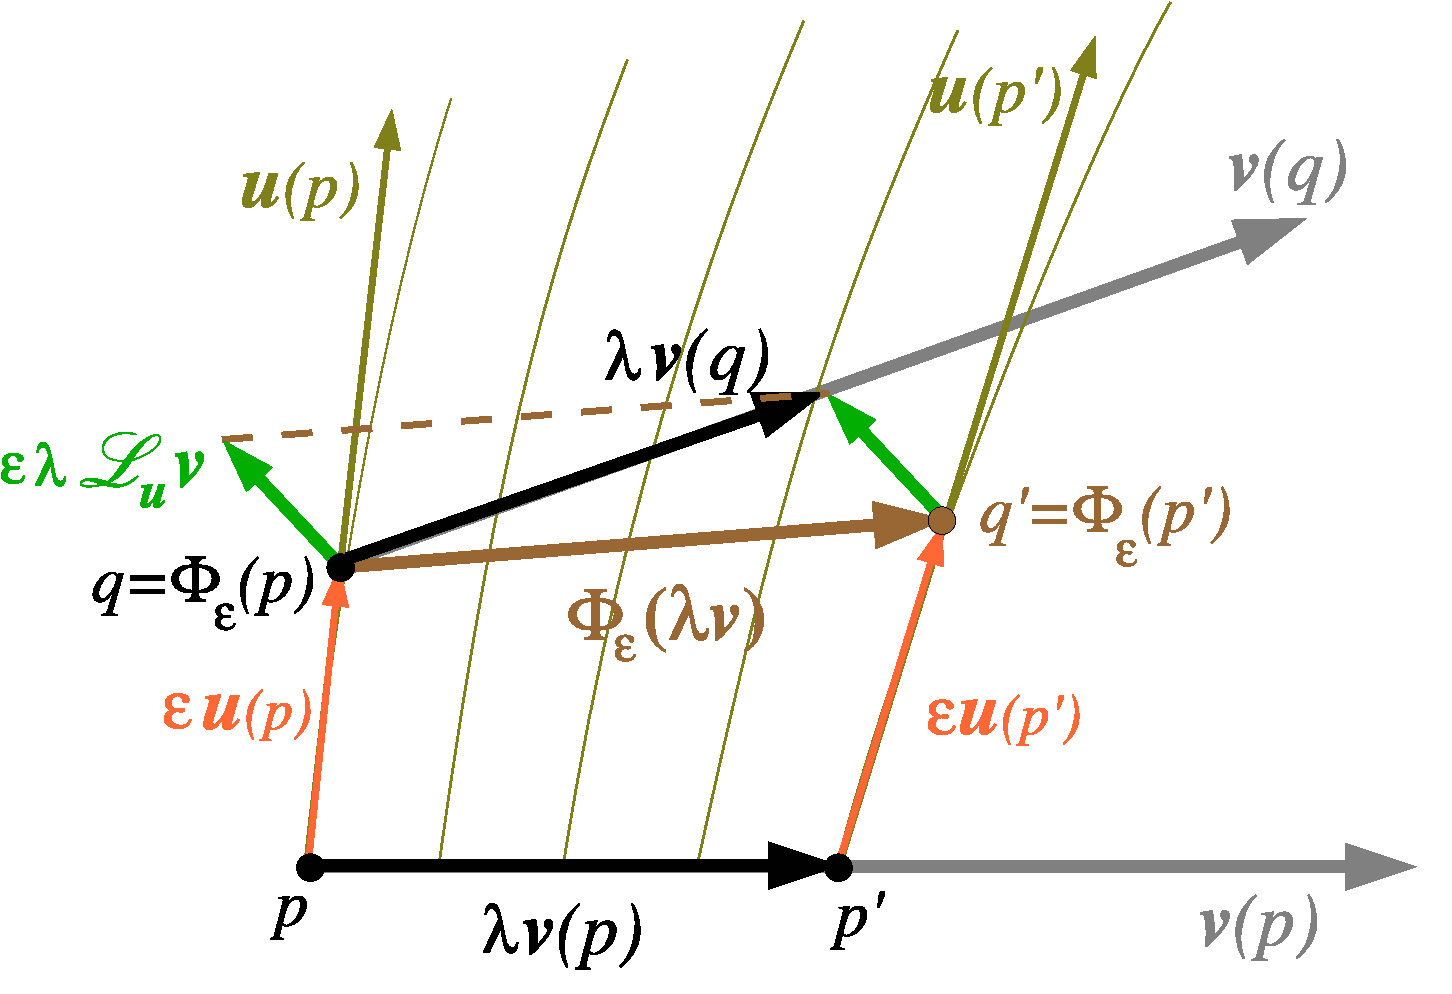
\includegraphics[width=0.6\textwidth]{bas_lie_deriv.pdf}}
\caption[]{\label{f:bas:deriv}
\footnotesize
Geometrical construction of the Lie derivative of a
vector field: given a small parameter $\lambda$, each extremity of the arrow
$\lambda\w{v}$ is dragged by some small parameter $\varepsilon$
along $\w{u}$, to form
the vector denoted by $\Phi_\varepsilon^*(\lambda\w{v})$. The latter is then compared with
the actual value of $\lambda\w{v}$ at the point $q$, the difference (divided
by $\lambda\varepsilon$) defining the Lie derivative $\Lie{u}\w{v}$.}
\end{figure}


Let us consider a coordinate system $(x^\alpha)$ adapted to the
field $\w{u}$ in the sense that $\w{u}=\wpar_0$, where $\wpar_0$ is the first
vector of the natural basis associated with the coordinates $(x^\alpha)$.
We have, from the definitions of points $q$, $p'$ and $q'$,
\bea
  & & x^\alpha(q) = x^\alpha(p)+\varepsilon \delta^\alpha_{\ \ 0}  \nonumber \\
  & & x^\alpha(p')= x^\alpha(p)+ \lambda v^\alpha(p) \nonumber \\
  & & x^\alpha(q')= x^\alpha(p')+\varepsilon \delta^\alpha_{\ \ 0} ,\nonumber
\eea
so that
\[
  (qq')^\alpha = x^\alpha(p')-x^\alpha(p) = \lambda v^\alpha(p) .
\]
Accordingly, (\ref{e:bas:def_Phi_eps}) and (\ref{e:bas:def_Lie_der}) result in
\bea
  \left( \Lie{u} \w{v} \right)^\alpha & = &\lim_{\varepsilon\rightarrow 0} \frac{1}{\varepsilon}
  \left[ v^\alpha(q) - v^\alpha(p) \right] \nonumber \\
  & = &
  \lim_{\varepsilon\rightarrow 0} \frac{1}{\varepsilon}
  \left[ v^\alpha(x^0+\varepsilon,\; x^1,\; \ldots,\; x^{n-1}) -
  v^\alpha(x^0, \; x^1,\; \ldots,\; x^{n-1}) \right] . \nonumber
\eea
Hence, in adapted coordinates, the Lie derivative is simply obtained by taking the partial derivative of the vector components
with respect to $x^0$:
\be \label{e:bas:Lie_adapted_vec}
	\Liec{u} v^\alpha  = \der{v^\alpha}{x^0} ,
\ee
where we have used the standard notation for the components of a Lie derivative:
$\Liec{u} v^\alpha := \left( \Lie{u} \w{v} \right)^\alpha$.
Besides, using the fact that the components of $\w{u}$
are $u^\alpha=(1,0,\ldots,0)$ in the adapted coordinate system, we notice that the components
of the commutator of $\w{u}$ and $\w{v}$, as given by (\ref{e:bas:commut_comp}), are
\[
  [\w{u},\w{v}]^\alpha = \der{v^\alpha}{x^0} .
\]
This is exactly (\ref{e:bas:Lie_adapted_vec}): $[\w{u},\w{v}]^\alpha = \Liec{u} v^\alpha$. We conclude that the Lie derivative of a vector with respect to another
one is actually nothing but the commutator of these two vectors:
\be \label{e:bas:Lie_commut}
	\encadre{ \Lie{u} \w{v} = [\w{u},\w{v}] } .
\ee
Thanks to formula (\ref{e:bas:commut_comp}), we may then express the components of the Lie
derivative in an arbitrary coordinate system:
\be \label{e:bas:Lie_vect}
	\encadre{ \Liec{u} v^\alpha = u^\mu \der{v^\alpha}{x^\mu}
	- v^\mu \der{u^\alpha}{x^\mu} } .
\ee

Thanks to the symmetry property of the Christoffel symbols,
the partial derivatives in Eq.~(\ref{e:bas:Lie_vect}) can be
replaced by the Levi-Civita connection
$\wnab$ associated with some metric $\w{g}$, yielding
\be \label{e:bas:Lie_vect_nab}
  \Liec{u} v^\alpha = u^\mu \nabla_\mu v^\alpha
	- v^\mu \nabla_\mu u^\alpha .
\ee

\subsubsection{Generalization to any tensor field}

If $\w{T}$ is tensor field of type $(0,\ell)$ on $\M$ (with $\ell \geq 1$)
its \defin{pullback}\index{pullback}
by the flow map
$\Phi_\varepsilon$ is the tensor field $\Phi_\varepsilon^*\w{T}$ of type $(0,\ell)$
defined by applying $\w{T}$ to pushforwarded vectors:
\be \label{e:bas:def_pullback}
    \forall (\w{v}_1,\ldots,\w{v}_\ell)\in (T_p\M)^\ell,\quad
    \left. \Phi_\varepsilon^*\w{T}\right| _p(\w{v}_1,\ldots,\w{v}_\ell) :=
        \left.\w{T}\right| _{\Phi_\varepsilon(p)} \left( \Phi_\varepsilon^*(\w{v}_1),
         \ldots, \Phi_\varepsilon^*(\w{v}_\ell) \right) .
\ee
The \defin{Lie derivative} of $\w{T}$ along $\w{u}$ is then defined
by comparing the pullback image at some point $p$ to the actual value
of $\w{\omega}$ at the same point:
\be \label{e:bas:def_Lie_der_covar}
    \encadre{ \Lie{u} \w{T} := \lim_{\varepsilon\rightarrow 0} \frac{1}{\varepsilon}
    \left( \Phi_\varepsilon^*\w{T} - \w{T} \right) }.
\ee

Finally, the Lie derivative is extended to any tensor field by (i) demanding that for
a scalar field $f$, $\Lie{u} f = \langle\wnab f,\w{u}\rangle$ and (ii) using the Leibniz
rule. As a result, the Lie derivative $\Lie{u}\w{T}$ of a tensor field $\w{T}$ of type
$(k,\ell)$ is a tensor field of the same type, the components of which
with respect to a given coordinate system $(x^\alpha)$ are
\bea
\Liec{u} T^{\alpha_1\ldots\alpha_k}_{\qquad\ \; \beta_1\ldots\beta_\ell} &=&
u^\mu \der{}{x^\mu} T^{\alpha_1\ldots\alpha_k}_{\qquad\ \; \beta_1\ldots\beta_\ell}
- \sum_{i=1}^k T^{\alpha_1\ldots
\!{{{\scriptstyle i\atop\downarrow}\atop \scriptstyle\sigma}\atop\ }\!\!
\ldots\alpha_k}_{\qquad\ \ \ \  \  \  \; \beta_1\ldots\beta_\ell}
 \; \der{u^{\alpha_i}}{x^\sigma} \nonumber \\
 & &  +  \sum_{i=1}^\ell T^{\alpha_1\ldots\alpha_k}_{\qquad\ \; \beta_1\ldots
\!{\ \atop {\scriptstyle\sigma \atop {\uparrow\atop \scriptstyle i}} }\!\!
\ldots\beta_\ell}
\; \der{u^{\sigma}}{x^{\beta_i}} . \label{e:Lie_der_comp}
\eea
In particular, for a 1-form,
\be \label{e:Lie_der_1form}
	\Liec{u} \omega_\alpha = u^\mu \der{\omega_\alpha}{x^\mu}
	+ \omega_\mu \der{u^\mu}{x^\alpha} .
\ee
As for the vector case [Eq.~(\ref{e:bas:Lie_vect})], the
partial derivatives in Eq.~(\ref{e:Lie_der_comp}) can be
replaced by the covariant derivative $\wnab$ (or any other connection without torsion),
yielding
\bea
\Liec{u} T^{\alpha_1\ldots\alpha_k}_{\qquad\ \; \beta_1\ldots\beta_\ell} &=&
u^\mu \nabla_\mu T^{\alpha_1\ldots\alpha_k}_{\qquad\ \; \beta_1\ldots\beta_\ell}
- \sum_{i=1}^k T^{\alpha_1\ldots
\!{{{\scriptstyle i\atop\downarrow}\atop \scriptstyle\sigma}\atop\ }\!\!
\ldots\alpha_k}_{\qquad\ \ \ \  \  \  \; \beta_1\ldots\beta_\ell}
 \; \nabla_\sigma u^{\alpha_i} \nonumber \\
 & & +  \sum_{i=1}^\ell T^{\alpha_1\ldots\alpha_k}_{\qquad\ \; \beta_1\ldots
\!{\ \atop {\scriptstyle\sigma \atop {\uparrow\atop \scriptstyle i}} }\!\!
\ldots\beta_\ell}
\; \nabla_{\beta_i} u^{\sigma} . \label{e:bas:Lie_der_comp_nab}
\eea

In adapted coordinates, we have, similarly to Eq.~(\ref{e:bas:Lie_adapted_vec}),
\be \label{e:bas:Lie_adapted}
    \Liec{u} T^{\alpha_1\ldots\alpha_k}_{\qquad\ \; \beta_1\ldots\beta_\ell}
     = \der{}{x^0} T^{\alpha_1\ldots\alpha_k}_{\qquad\ \; \beta_1\ldots\beta_\ell}
     \qquad \mbox{(coordinates adapted to $\w{u}$)}.
\ee
Note that this formula is a direct consequence of (\ref{e:Lie_der_comp})
since in adapted coordinates, $u^\alpha = (1,0,\ldots,0)$, so that
$u^\mu \dert{}{x^\mu} = \dert{}{x^0}$ and $\dert{u^\alpha}{x^\beta} = 0$.



\subsection{Exterior derivative} \label{s:bas:ext_deriv}

In Sec.~\ref{s:bas:fields}, we have introduced the
\emph{differential forms}\index{differential!form}\index{form!differential}
as tensor fields of type $(0,q)$, with $q\ge 0$,
that are antisymmetric in all their arguments as soon as $q\ge 2$.
Otherwise stating, at each point $p\in\M$, a differential form results in a
fully antisymmetric multilinear form on the vector space $T_p\M$.
A differential form of order $q$ is also called a $q$-form.

Differential forms play a special role in the theory of integration on a
manifold. Indeed the primary definition of an integral over a manifold of
dimension $n$ is the integral of a $n$-form. The Levi-Civita tensor
$\w{\epsilon}$
introduced in Sec.~\ref{s:bas:Levi-Civita_tensor} is a $n$-form, whose integral
gives the volume with respect to the metric $\w{g}$.
Regarding physics, it is well known that the
electromagnetic field is fundamentally a 2-form (the Faraday tensor $\w{F}$);
in relativistic hydrodynamics, the vorticity of a fluid is also described by a 2-form
(see e.g. \cite{Gourg13}).

Being tensor fields, differential forms are subject to the covariant
and Lie derivations discussed above. But, in addition, they are subject to a third type
of derivation, called \emph{exterior derivation}.
The \defin{exterior derivative}\index{exterior!derivative}\index{derivative!exterior}
 of a $q$-form $\w{\omega}$ is a
$(q+1)$-form which is denoted $\dd\w{\omega}$ and whose components
with respect to a given coordinate system $(x^\alpha)$ are defined by
\bea
	\mbox{0-form (scalar field)} & : & (\dd\w{\omega})_\alpha =
		\der{\omega}{x^\alpha} \label{e:bas:def_ext_0f} \\
	\mbox{1-form} & : & (\dd\w{\omega})_{\alpha\beta} =
	\der{\omega_\beta}{x^\alpha} - \der{\omega_\alpha}{x^\beta}
			 \label{e:bas:def_ext_1f} \\
	\mbox{2-form} & : & (\dd\w{\omega})_{\alpha\beta\gamma} =
	\der{\omega_{\beta\gamma}}{x^\alpha} +
	\der{\omega_{\gamma\alpha}}{x^\beta} +
	\der{\omega_{\alpha\beta}}{x^\gamma} \label{e:bas:def_ext_2f} \\
	\mbox{etc...}
\eea
It can be easily checked that these formul\ae, although expressed in terms of
partial derivatives of components in a coordinate system, do define tensor fields.
Moreover, the result is clearly antisymmetric (assuming that $\w{\omega}$ is), so
that we end up with $(q+1)$-forms.
Notice that for a scalar field (0-form), the exterior derivative is nothing but the
differential 1-form $\dd f$ already defined in Sec.~\ref{s:bas:linear_form}.
Notice also that the definition of the exterior derivative appeals only to the
manifold structure. It does not depend upon the metric tensor  $\w{g}$, nor upon
any other extra structure on $\M$. We may also notice that
all partial derivatives in the formul\ae\
(\ref{e:bas:def_ext_0f})-(\ref{e:bas:def_ext_2f}) can be replaced by covariant derivatives
(thanks to the symmetry of the Christoffel symbols).

A fundamental property of the exterior derivation is to be nilpotent:
\be \label{e:ext_der_nilpot}
	\encadre{ \dd\dd\w{\omega} = 0 }.
\ee
A $q$-form $\w{\omega}$ is said to be \emph{closed} iff $\dd\w{\omega}=0$,
and \emph{exact} iff there exists a $(q-1)$-form $\w{\sigma}$ such that
$\w{\omega} = \dd\w{\sigma}$. From property (\ref{e:ext_der_nilpot}),
an exact $q$-form is closed. The Poincar\'e lemma states that the converse is true,
at least locally.

The exterior derivative enters in the well known \emph{Stokes' theorem}\index{Stokes!theorem}: if $\mathcal{D}$
is a submanifold of $\M$ of dimension $d$ that has a boundary (denoted $\partial\mathcal{D}$), then for any $(d-1)$-form $\w{\omega}$,
\be \label{e:Stokes}
	\oint_{\partial\mathcal{D}} \w{\omega} =
	\int_{\mathcal{D}} \dd\w{\omega} .
\ee
Note that $\partial\mathcal{D}$ is a manifold of dimension $d-1$ and
$\dd\w{\omega}$ is a $d$-form, so that each side of
(\ref{e:Stokes}) is (of course !) a well defined quantity,
as the integral of a $q$-form over a $q$-dimensional manifold.

Another very important formula where the exterior derivative enters is
the \defin{Cartan identity}\index{Cartan!identity}, which states that the
Lie derivative of a differential form
$\w{\omega}$ along a vector field $\w{u}$ is expressible as
\be \label{e:Cartan}
	\encadre{ \Lie{u}\w{\omega} = \w{u}\cdot\dd\w{\omega}
	+ \dd(\w{u}\cdot\w{\omega}) }.
\ee
In the above formula, a dot denotes the contraction on adjacent indices, i.e.
$\w{u}\cdot\w{\omega}$ is the $(q-1)$-form $\w{\omega}(\w{v},.,\ldots,.)$,
with the $q-1$ last slots remaining free. Notice that in
the case of a 1-form, Eq.~(\ref{e:Cartan}) is readily obtained
by combining Eqs.~(\ref{e:Lie_der_1form}),
(\ref{e:bas:def_ext_0f}) and (\ref{e:bas:def_ext_1f}).

%%%%%%%%%%%%%%%%%%%%%%%%%%%%%%%%%%%%%%%%%%%%%%%%%%%%%%%%%%%%%%%%%%%%%%%%%%%%%%%

\section{Curvature} \label{s:bas:curvat}

\subsection{General definition}

The \defin{Riemann curvature tensor}\index{Riemann!curvature}\index{curvature!tensor} of
an affine connection $\w{\nabla}$ is defined by
\be \label{e:bas:def_Riemann}
	 \begin{array}{cccc}
	\mathrm{\bf Riem} \ : & \mathscr{X}^*(\M)\times\mathscr{X}(\M)^3 &
	\longrightarrow & C^\infty(\M,\R) \\
		& (\w{\omega},\w{w},\w{u},\w{v})
		& \longmapsto & \bigg\langle \w{\omega} , \
                \w{\nabla}_{\w{u}} \w{\nabla}_{\w{v}} \w{w}
		-  \w{\nabla}_{\w{v}} \w{\nabla}_{\w{u}} \w{w}
		- \w{\nabla}_{[\w{u},\w{v}]} \w{w} \bigg\rangle ,
	\end{array}
\ee
where $\mathscr{X}^*(\M)$ stands for the space of 1-forms on $\M$, $\mathscr{X}(\M)$ for the space of vector
fields on $\M$ and  $C^\infty(\M,\R)$ for the space of
smooth scalar fields on $\M$. The above
formula does define a tensor field on $\M$, i.e. the value
of $\mathrm{\bf Riem}(\w{\omega},\w{w},\w{u},\w{v})$ at a given
point $p\in\M$ depends only upon the values of the fields
$\w{\omega}$, $\w{w}$, $\w{u}$ and $\w{v}$ at $p$ and not
upon their behaviours away from $p$, as the covariant derivatives in
Eq.~(\ref{e:bas:def_Riemann}) might suggest.
We denote the components of this tensor in
a given basis $(\w{e}_\alpha)$, not by
${\rm Riem}^\gamma_{\ \  \delta \alpha\beta}$, but by
$R^\gamma_{\ \  \delta \alpha\beta}$.
The definition (\ref{e:bas:def_Riemann}) leads then to the
following expression, named the \defin{Ricci identity}\index{Ricci!identity}:
\be \label{e:bas:Ricci_ident}
    \forall\w{w}\in\mathscr{X}(\M),\quad
        \left(\nabla_\alpha\nabla_\beta
        - \nabla_\beta\nabla_\alpha\right) w^\gamma
        = R^\gamma_{\ \  \mu \alpha\beta} \, w^\mu .
\ee
\begin{remark}
In view of this identity, one may say that the Riemann tensor measures the lack of
commutativity of two successive covariant derivatives of a vector field.
On the opposite,
for a scalar field and a torsion-free connection,
two successive covariant derivatives always commute [cf. Eq.~(\ref{e:bas:torsion-free})].
\end{remark}
In a coordinate basis, the components of the Riemann tensor are given in terms of the connection
coefficients by
\be \label{e:bas:Riemann_comp}
  	\encadre{ R^\alpha_{\ \  \beta\mu\nu}  =
	\der{\Gamma^\alpha_{\ \  \beta\nu}}{x^\mu}
	- \der{\Gamma^\alpha_{\ \  \beta\mu}}{x^\nu}
	+ \Gamma^\alpha_{\ \  \sigma\mu} \Gamma^\sigma_{\ \  \beta\nu}
	- \Gamma^\alpha_{\ \  \sigma\nu} \Gamma^\sigma_{\ \  \beta\mu}  } .
\ee

From the definition (\ref{e:bas:def_Riemann}), the Riemann tensor is
clearly antisymmetric with respect to its last two arguments $(\w{u},\w{v})$:
\be \label{e:bas:Riemann_antisym34}
  \mathrm{\bf Riem}(.,.,\w{u},\w{v}) = - \mathrm{\bf Riem}(.,.,\w{v},\w{u}) .
\ee
In addition, it satisfies the cyclic property
\be \label{e:bas:Riemann_cyclic}
\mathrm{\bf Riem}(.,\w{u},\w{v},\w{w})
+\mathrm{\bf Riem}(.,\w{w},\w{u},\w{v})
+\mathrm{\bf Riem}(.,\w{v},\w{w},\w{u}) = 0 .
\ee
The covariant derivatives of the Riemann tensor obeys the \defin{Bianchi identity}\index{Bianchi identity}
\be \label{e:bas:Bianchi}
    \encadre{ \nabla_\rho  R^\alpha_{\ \  \beta\mu\nu}
	+ \nabla_\mu R^\alpha_{\ \ \beta\nu\rho}
	+ \nabla_\nu R^\alpha_{\ \ \beta\rho\mu} =0 }.
\ee

\subsection{Case of a pseudo-Riemannian manifold}

The Riemann tensor of the Levi-Civita connection obeys the additional antisymmetry:
\be \label{e:bas:Riemann_antisym12}
    \mathrm{\bf Riem}(\w{\omega},\w{w},.,.)
    = - \mathrm{\bf Riem}(\uu{w},\vw{\omega},.,.) .
\ee
Combined with (\ref{e:bas:Riemann_antisym34}) and (\ref{e:bas:Riemann_cyclic}), this implies
the symmetry property
\be \label{e:bas:Riemann_sym}
  \mathrm{\bf Riem}(\w{\omega},\w{w},\w{u},\w{v}) =
  \mathrm{\bf Riem}(\uu{u},\w{v},\vw{\omega},\w{w}) .
\ee

A pseudo-Riemannian manifold $(\M,\w{g})$ with a vanishing Riemann tensor is called
a \defin{flat manifold}\index{flat!manifold}; in this case, $\w{g}$ is said to be
a \defin{flat metric}\index{flat!metric}. If in addition, it has a Riemannian signature,
$\w{g}$ is called an
\defin{Euclidean metric}\index{Euclidean!metric}.

\subsection{Ricci tensor} \label{s:bas:Ricci_tensor}

The \defin{Ricci tensor}\index{Ricci!tensor} of the affine connection $\wnab$ is
the field of bilinear forms $\w{R}$ defined by
\be \label{e:bas:def_Ricci}
	 \begin{array}{cccc}
	\w{R} \ : & \mathscr{X}(\M)\times\mathscr{X}(\M) &
	\longrightarrow & C^\infty(\M,\R) \\
		& (\w{u},\w{v})
		& \longmapsto &
                \mathrm{\bf Riem}(\w{e}^\mu,\w{u},\w{e}_\mu,\w{v}) ,
	\end{array}
\ee
where $(\w{e}_\alpha)$ is a vector frame on $\M$ and $(\w{e}^\alpha)$
its dual counterpart.
This definition is independent of the choice of $(\w{e}_\alpha)$.
In terms of components:
\be \label{e:bas:def_Ricci_comp}
    \encadre{ R_{\alpha\beta} := R^\mu_{\ \  \alpha\mu\beta} }.
\ee
\begin{remark}
Following the standard usage, we denote the components
of the Riemann and Ricci tensors by the same letter $R$, the
number of indices allowing us to distinguish between the two tensors.
On the other hand, we are using different symbols, $\mathrm{\bf Riem}$ and
$\w{R}$, when employing the `intrinsic' notation.
\end{remark}

For the Levi-Civita connection associated with the metric $\w{g}$, the property (\ref{e:bas:Riemann_sym}) implies that the Ricci tensor is symmetric:
\be
  \w{R}(\w{u},\w{v}) = \w{R}(\w{v},\w{u}) .
\ee
In addition, one defines the
\defin{Ricci scalar}\index{Ricci!scalar}
(also called \defin{scalar curvature}\index{scalar!curvature}\index{curvature!scalar})
as the trace of the Ricci tensor with respect to the metric $\w{g}$:
\be \label{e:bas:def_Ricci_scal}
  R :=g^{\mu\nu} R_{\mu\nu} .
\ee
The Bianchi identity (\ref{e:bas:Bianchi}) implies the divergence-free property
\be \label{e:bas:Bianchi_contr}
  \encadre{ \wnab\cdot\vw{G} = 0 },
\ee
where $\vw{G}$ in the type-$(1,1)$ tensor associated by metric duality
[cf. (\ref{e:bas:arrow_endo})] to
the \defin{Einstein tensor}\index{Einstein!tensor}:
\be \label{e:bas:Einstein_tensor}
  \encadre{ \w{G} := \w{R} - \frac{1}{2} R\, \w{g} } .
\ee
Equation~(\ref{e:bas:Bianchi_contr}) is called the \defin{contracted Bianchi identity}\index{contracted!Bianchi identity}\index{Bianchi identity!contracted}.

\subsection{Weyl tensor} \label{s:bas:Weyl}

Let $(\M,\w{g})$ be a pseudo-Riemannian manifold of dimension $n$.

For $n=1$, the Riemann tensor vanishes identically, i.e. $(\M,\w{g})$  is
necessarily flat.
The reader who has in mind a curved line in the Euclidean plane $\R^2$ might be
surprised by the above statement. This is because the Riemann tensor
represents the  \emph{intrinsic} curvature\index{intrinsic curvature}\index{curvature!intrinsic} of a manifold. For a line, the
curvature that is not vanishing is the
\emph{extrinsic} curvature\index{extrinsic!curvature}\index{curvature!extrinsic}, i.e. the
curvature resulting from the embedding of the line in $\R^2$.

For $n=2$, the Riemann tensor is entirely determined by the knowledge of the
Ricci scalar $R$, according to the formula:
\be
  R^\gamma_{\ \; \delta\alpha\beta} =  R \left(
    \delta^\gamma_{\ \  \alpha} \, g_{\delta\beta}   -
    \delta^\gamma_{\ \  \beta} \, g_{\delta\alpha}
	     \right) \qquad (n=2) .
\ee

For $n=3$, the Riemann tensor is entirely determined by the knowledge of the
Ricci tensor, according to
\bea
  	R^\gamma_{\ \; \delta\alpha\beta}   & =&
	 R^\gamma_{\ \  \alpha} \, g_{\delta\beta}
	   - R^\gamma_{\ \  \beta}\,  g_{\delta\alpha}
	   + \delta^\gamma_{\ \  \alpha} \, R_{\delta\beta}
	   - \delta^\gamma_{\ \  \beta}  \, R_{\delta\alpha}
  \nonumber \\
     & &  + \frac{R}{2} \left(
  \delta^\gamma_{\ \  \beta} \, g_{\delta\alpha}
	   - \delta^\gamma_{\ \  \alpha} \, g_{\delta\beta}   \right)
   \qquad (n=3) . \label{e:bas:Riem_dim_3}
\eea

For $n\geq 4$, the Riemann tensor can
be split into (i) a ``trace-trace'' part, represented
by the Ricci scalar $R$ [Eq.~(\ref{e:bas:def_Ricci_scal})],
(ii) a ``trace'' part,
represented by the Ricci tensor $\w{R}$
[Eq.~(\ref{e:bas:def_Ricci_comp})], and (iii) a ``traceless'' part,
which is constituted by the \defin{Weyl conformal curvature tensor}\index{Weyl curvature tensor}\index{conformal!curvature}, $\w{C}$:
\bea
	R^\gamma_{\ \; \delta\alpha\beta}   & = &
        C^\gamma_{\ \; \delta\alpha\beta}
	+ \frac{1}{n-2} \left( R^\gamma_{\ \  \alpha} \, g_{\delta\beta}
	   - R^\gamma_{\ \  \beta}\,  g_{\delta\alpha}
	   + \delta^\gamma_{\ \  \alpha} \, R_{\delta\beta}
	   - \delta^\gamma_{\ \  \beta} \, R_{\delta\alpha}   \right)
                            \nonumber \\
	 &&   + \frac{1}{(n-1)(n-2)} R \left(
  \delta^\gamma_{\ \  \beta} \, g_{\delta\alpha}
	   - \delta^\gamma_{\ \  \alpha} \, g_{\delta\beta}   \right) . \label{e:bas:Weyl}
\eea
The above relation may be taken as the definition of $\w{C}$.
It implies that $\w{C}$ is traceless: $C^\mu_{\ \  \alpha\mu\beta}=0$.
The other possible traces are zero thanks to the symmetry properties of
the Riemann tensor.
\begin{remark}
The decomposition (\ref{e:bas:Weyl}) is also meaningful for $n=3$, but it then
implies that the Weyl tensor vanishes identically [compare with (\ref{e:bas:Riem_dim_3})].
\end{remark}

  % Basic differential geometry

\begin{thebibliography}{123}

\bibitem{AlexaIK14}
S. Alexakis, A. D. Ionescu, and S. Klainerman : {\em Rigidity of stationary black holes with small angular momentum on the horizon},
Duke Math. J. {\bf 163}, 2603 (2014)\\
DOI: \href{http://dx.doi.org/10.1215/00127094-2819517}{10.1215/00127094-2819517}

\bibitem{AshteBL02}
A. Ashtekar, C. Beetle, and J.~Lewandowski : {\em Geometry of
generic isolated horizons},
Class. Quantum Grav. {\bf 19}, 1195 (2002).

\bibitem{AshteFK00}
A. Ashtekar, S. Fairhurst, and B. Krishnan : {\em Isolated horizons:
Hamiltonian evolution and the first law},
Phys. Rev. D {\bf 62}, 104025 (2000).

\bibitem{AshteK04}
A. Ashtekar and B. Krishnan : {\em Isolated and dynamical horizons
and their applications},
Living Rev. Relativity {\bf 7}, 10 (2004) \\
\url{http://www.livingreviews.org/lrr-2004-10}

\bibitem{Bard15}
G.V. Bard : {\em Sage for Undergraduates}, Americ. Math. Soc. (2015); \\
preprint freely downloadable from \url{http://www.gregorybard.com/}

\bibitem{BardeCH73}
J.W. Bardeen, B. Carter, and S.W. Hawking : {\em The four laws of black
hole mechanics}, Commun. Math. Phys., {\bf 31}, 161 (1973).

\bibitem{Berge03}
M. Berger : {\em A Panoramic View of Riemannian Geometry},
Springer, Berlin (2003).

\bibitem{Boyer69}
R.H. Boyer : {\em Geodesic Killing orbits and bifurcate Killing horizons},
Proc. Roy. Soc. A {\bf 311}, 245 (1969)\\
DOI: \href{http://dx.doi.org/10.1098/rspa.1969.0116}{10.1098/rspa.1969.0116}

\bibitem{BoyerP65}
R.H. Boyer and T.G. Price : {\em An interpretation of the Kerr metric in general relativity},
Math. Proc. Cambridge Phil. Soc. {\bf 61}, 531 (1965)\\
DOI: \href{http://dx.doi.org/10.1017/S0305004100004096}{10.1017/S0305004100004096}

\bibitem{Brill14}
D. Brill : {\em History of a black hole horizon},
Grav. Cosmo. {\bf 20}, 165 (2014)
DOI: \href{http://dx.doi.org/10.1134/S0202289314030050}{10.1134/S0202289314030050}

\bibitem{Carro04}
S.M. Carroll : \emph{Spacetime and Geometry: An Introduction to General Relativity},
Addison Wesley (Pearson Education), San Fransisco (2004); \\
\url{http://preposterousuniverse.com/spacetimeandgeometry/}

\bibitem{Carte66}
B.~Carter :
{\em Complete Analytic Extension of the Symmetry Axis of Kerr's Solution of Einstein's Equations},
Phys. Rev. {\bf 141}, 1242 (1966)\\
DOI: \href{http://dx.doi.org/10.1103/PhysRev.141.1242}{10.1103/PhysRev.141.1242}

\bibitem{Carte67}
B.~Carter : {\em Stationary Axisymmetric Systems in General Relativity},
Ph. D. Thesis, Cambridge University (1967); available at\\
\url{http://luth.obspm.fr/~luthier/carter/Thesis/}

\bibitem{Carte68}
B.~Carter :
{\em Global Structure of the Kerr Family of Gravitational Fields},
Phys. Rev. {\bf 174}, 1559 (1968)\\
DOI: \href{http://dx.doi.org/10.1103/PhysRev.174.1559}{10.1103/PhysRev.174.1559}

\bibitem{Carte69}
B.~Carter : {\em Killing horizons and orthogonally transitive groups
in space-time},
J. Math. Phys. {\bf 10}, 70 (1969).

\bibitem{Carte71}
B.~Carter : {\em Axisymmetric Black Hole Has Only Two Degrees of Freedom},
Phys. Rev. Lett. {\bf 26}, 331 (1971)\\
DOI: \href{http://dx.doi.org/10.1103/PhysRevLett.26.331}{10.1103/PhysRevLett.26.331}

\bibitem{Carte73a}
B.~Carter : {\em Black hole equilibrium states Part I.
Analytic and Geometric Properties of the Kerr Solutions},
in {\em Black Holes -- Les astres occlus},  edited by C.~DeWitt and B.~DeWitt,
Gordon and Breach, New York (1973), p.~57; reprinted (with corrections) in
Gen. Relativ. Gravit. {\bf 41}, 2873 (2009)\\
DOI: \href{http://dx.doi.org/doi:10.1007/s10714-009-0888-5}{10.1007/s10714-009-0888-5}

\bibitem{Carte73b}
B.~Carter : {\em Black hole equilibrium states Part II. General theory of stationary black hole states}, in {\em Black Holes -- Les astres occlus},  edited by C.~DeWitt and B.~DeWitt,
Gordon and Breach, New York (1973), p.~125; reprinted (with corrections) in
Gen. Relativ. Gravit. {\bf 42}, 653 (2010)\\
DOI: \href{http://dx.doi.org/doi:10.1007/s10714-009-0920-9}{10.1007/s10714-009-0920-9}

\bibitem{Carte87}
B.~Carter : {\em Mathematical foundations of the theory of
relativistic stellar and black hole configurations},
in {\em Gravitation in Astrophysics}, Eds. B.~Carter and J.B.~Hartle,
Plenum Press, New York (1987).

\bibitem{Carte97}
B. Carter : {\em Extended tensorial curvature analysis for embeddings
and foliations},
Contemp. Math. {\bf 203}, 207 (1997).

\bibitem{Carte99}
B. Carter : {\em Has the black hole equilibrium problem been solved?},
in {\em The Eighth Marcel Grossmann Meeting}, edited by T.~Piran,
World Scientific, Singapore (1999);\\
preprint: \url{http://arxiv.org/abs/gr-qc/9712038}

\bibitem{Choqu09}
Y. Choquet-Bruhat : {\em General Relativity and Einstein's Equations},
Oxford Univ. Press, New York (2009).

\bibitem{Choqu15}
Y. Choquet-Bruhat : {\em Introduction to General Relativity, Black Holes, and
Cosmology}, Oxford Univ. Press, New York (2015).

\bibitem{ChoquDD77}
Y. Choquet-Bruhat, C. De Witt-Moretten, and M. Dillard-Bleick :
{\em Analysis, Manifolds and Physics},
North-Holland, Amsterdam (1977).

\bibitem{Chrus97}
P.T. Chru\'sciel : {\em On Rigidity of Analytic Black Holes},
Commun. Math. Phys. {\bf 189}, 1 (1997) \\
DOI: \href{http://dx.doi.org/10.1007/s002200050187}{10.1007/s002200050187}

\bibitem{Chrus02}
P.T. Chru\'sciel : {\em Black holes},
in {\em Proceedings of the T\"ubingen conference on conformal structure of
space-time}, edited by J.~Frauendiener, H.~Friedrich,
Lecture Notes in Physics {\bf 604}, 61,
Springer, Berlin (2002).

\bibitem{Chrus05}
P.T. Chru\'sciel : {\em Black holes -- An Introduction},
in {\em 100 Years of Relativity}, edited by A. Ashtekar,
World Scientific, Singapore (2005), p. 93\\
DOI: \href{http://dx.doi.org/doi:10.1142/9789812700988_0004}{10.1142/9789812700988\_0004}

\bibitem{ChrusDGH01}
P. Chru\'sciel, E. Delay, G. Galloway and R. Howard :
{\em Regularity of horizons and the area theorem},
Annales Henri Poincar\'e {\bf 2}, 109 (2001)\\
DOI: \href{http://dx.doi.org/10.1007/PL00001029}{10.1007/PL00001029}

\bibitem{ChrusG10}
P. Chru\'sciel and G.J. Galloway :
{\em Uniqueness of static black holes without analyticity},
Class. Quantum Grav. {\bf 27}, 152001 (2010)\\
DOI: \href{http://dx.doi.org/10.1088/0264-9381/27/15/152001}{10.1088/0264-9381/27/15/152001}

\bibitem{ChrusLH12}
P.T. Chru\'sciel, J. Lopes Costa, and M. Heusler :
{\em Stationary Black Holes: Uniqueness and Beyond},
Living Rev. Relativity {\bf 15}, 7 (2012) \\
\url{http://www.livingreviews.org/lrr-2012-7}

\bibitem{ChrusN10}
P.T. Chru\'sciel and L. Nguyen :
{\em A Uniqueness Theorem for Degenerate Kerr–Newman Black Holes},
Ann. Henri Poincar\'e {\bf 11}, 585 (2010)\\
DOI: \href{http://dx.doi.org/10.1007/s00023-010-0038-3}{10.1007/s00023-010-0038-3}

\bibitem{CohenKS12}
M.I. Cohen, J.D. Kaplan, and M.A. Scheel :
{\em Toroidal horizons in binary black hole inspirals},
Phys. Rev. D {\bf 85}, 024031 (2012)\\
DOI:  \href{http://dx.doi.org/10.1103/PhysRevD.85.024031}{10.1103/PhysRevD.85.024031}

\bibitem{CohenPS09}
M.I. Cohen, H.P. Pfeiffer and M.A. Scheel :
{\em Revisiting event horizon finders},
Class. Quantum Grav. {\bf 26}, 035005 (2009)\\
DOI: \href{http://dx.doi.org/10.1088/0264-9381/26/3/035005}{10.1088/0264-9381/26/3/035005}

\bibitem{CollaK12}
P. Collas and D. Klein :
{\em Embeddings and time evolution of the Schwarzschild wormhole},
Amer. J. Phys. {\bf 80}, 203 (2012)\\
DOI: \href{http://dx.doi.org/10.1119/1.3672848}{10.1119/1.3672848}

\bibitem{CorleGHJK965}
R.M. Corless, G.H. Gonnet, D.E.G. Hare, D.J. Jeffrey and D.E. Knuth :
{\em On the Lambert W function},
Adv. Comput. Math. {\bf 5}, 329 (1996)\\
DOI: \href{http://dx.doi.org/10.1007/BF02124750}{10.1007/BF02124750}

\bibitem{DaferR13}
M. Dafermos and I. Rodnianski : {\em Lecture on black holes and linear waves},
in  Clay Math. Proc. {\bf 17}: {\em Evolution Equations}, edited by
D. Ellwood, I. Rodnianski, G. Staffilani and J. Wunsch, AMS / Clay Mathematical Institute,
Cambridge (2013) \\
\url{http://people.maths.ox.ac.uk/cmi/library/proceedings/cmip017c.pdf}

\bibitem{Damou79}
T. Damour : {\em Quelques propri\'et\'es m\'ecaniques, \'electromagn\'etiques,
thermo\-dy\-na\-mi\-ques et quantiques des trous noirs},
Th\`ese de doctorat d'\'Etat, Universit\'e Paris 6 (1979); available at\\
\url{http://pagesperso.ihes.fr/~damour/Articles/}

\bibitem{Damou82}
T. Damour : {\em Surface effects in black hole physics},
in {\em Proceedings of the Second Marcel Grossmann Meeting on General
Relativity}, Ed. R.~Ruffini, North Holland (1982), p.~587; available at\\
\url{http://pagesperso.ihes.fr/~damour/Articles/}

\bibitem{Damou04}
T. Damour : {\em The Entropy of Black Holes: A Primer},
in {\em Poincaré Seminar 2003: Bose-Einstein Condensation -- Entropy},
edited by J. Dalibard, B. Duplantier and V. Rivasseau, Birkha\"auser, Basel (2004),
p.~227

\bibitem{Derue09}
N. Deruelle : {\em Black Holes in General Relativity}, lectures at
Institut de Physique Théorique, CEA, Saclay (France) (2009); slides and notes
available at \\
\url{http://ipht.cea.fr/Docspht/search/article.php?id=t09/346}

\bibitem{DerueU14}
N. Deruelle and J.-P. Uzan : {\em Th\'eories de la Relativit\'e},
Belin, Paris (2014).

\bibitem{DeWit73}
C.~DeWitt and B.~DeWitt (eds.) :
{\em Black Holes -- Les astres occlus},
Gordon and Breach, New York (1973).

\bibitem{Drost1917}
J. Droste :
{\em The Field of a Single Centre in Einstein's Theory of Gravitation, and the Motion of a Particle in that Field},
Koninklijke Nederlandsche Akademie van Wetenschappen Proceedings {\bf 19}, 197 (1917);
reprinted in Gen. Relativ. Gravit. {\bf 34}, 1545 (2002)\\
DOI: \href{http://dx.doi.org/10.1023/A:1020747322668}{10.1023/A:1020747322668}

\bibitem{Eddin1924}
A.S. Eddington : {\em A comparison of Whitehead's and Einstein's Formul\ae},
Nature {\bf 113}, 192 (1924) \\
DOI: \href{http://dx.doi.org/10.1038/113192a0}{10.1038/113192a0}

\bibitem{EinstR35}
A. Einstein and N. Rosen :
{\em The Particle Problem in the General Theory of Relativity},
Phys. Rev. {\bf 48}, 73 (1935) \\
DOI: \href{https://doi.org/10.1103/PhysRev.48.73}{10.1103/PhysRev.48.73}

\bibitem{Eisen82}
J. Eisenstaedt :
{\em Histoire et Singularit\'es de la Solution de Schwarzschild (1915–1923)},
Archive for History of Exact Sciences {\bf 27}, 157 (1982) \\
DOI: \href{http://dx.doi.org/10.1007/BF00348347}{10.1007/BF00348347}

\bibitem{Eisen93}
J. Eisenstaedt : {\em Lemaître and the Schwarzschild Solution}, in
{\em The Attraction of Gravitation: New Studies in the History of
General Relativity}, Proc. Third International Conference on the History and Philosophy of General Relativity. Einstein
Studies, Vol. 5, edited by J.~Earman, M.~Janssen, and J.D.~Norton,
Birkhäuser, Boston (1993), p. 353.

\bibitem{Eschr11}
H. Eschrig : {\em Topology and Geometry for Physics},
Springer, Berlin (2011).

\bibitem{Finke58}
D. Finkelstein :
{\em Past-Future Asymmetry of the Gravitational Field of a Point Particle},
Phys. Rev. {\bf 110}, 965 (1958)\\
DOI: \href{http://dx.doi.org/10.1103/PhysRev.110.965}{10.1103/PhysRev.110.965}

\bibitem{Flamm1916}
L. Flamm : {\em Beiträge zur Einsteinschen Gravitationstheorie},
Physikalische Zeitschrift {\bf 17}, 448 (1916); English translation in
Gen. Relativ. Gravit. {\bf 47}, 72 (2015)\\
DOI: \href{http://dx.doi.org/10.1007/s10714-015-1908-2}{10.1007/s10714-015-1908-2}

\bibitem{Fraue04}
J. Frauendiener :
{\em Conformal Infinity},
Living Rev. Relativity {\bf 7}, 1 (2004) \\
\url{http://www.livingreviews.org/lrr-2004-1}

\bibitem{FroloN98}
V.P. Frolov and I.D. Novikov : {\em Black Hole Physics:
Basic Concepts and New Developments},
Kluwer Academic Publisher, Dordrecht (1998); reprinted by
Springer, Dordrecht (1998). \\
DOI: \href{http://dx.doi.org/10.1007/978-94-011-5139-9}{10.1007/978-94-011-5139-9}

\bibitem{FroloZ11}
V.P. Frolov and A. Zelnikov : {\em Introduction to Black Hole Physics},
Oxford University Press, New York (2011).

\bibitem{Frons59}
C. Fronsdal : {\em Completion and Embedding of the Schwarzschild Solution},
Phys. Rev. {\bf 116}, 778 (1959) \\
DOI: \href{https://doi.org/10.1103/PhysRev.116.778}{10.1103/PhysRev.116.778}

\bibitem{GerocH82}
R. Geroch and J.B. Hartle : {\em Distorted black holes},
J. Math. Phys. {\bf 23}, 680 (1982).

\bibitem{GibboW08}
G. Gibbons and C.M. Will : {\em On the Multiple Deaths of Whitehead's Theory of Gravity},
Studies in History and Philosophy of Science Part B: Studies in History and Philosophy of Modern Physics {\bf 39}, 41 (2008)\\
DOI: \href{http://dx.doi.org/doi:10.1016/j.shpsb.2007.04.004}{10.1016/j.shpsb.2007.04.004}

\bibitem{Gourg13}
E. Gourgoulhon : {\em Special Relativity in General Frames: From Particles to Astrophysics},
Springer, Berlin (2013) \\
\url{http://relativite.obspm.fr/sperel}

\bibitem{Gourg14}
E. Gourgoulhon : {\em Relativit\'e g\'en\'erale},
Master Lecture Notes\\
\url{http://luth.obspm.fr/~luthier/gourgoulhon/fr/master/relat.html}

\bibitem{GourgJ06}
E. Gourgoulhon and J.L. Jaramillo : {\em A 3+1 perspective on null hypersurfaces and isolated horizons},
Phys. Rep. {\bf 423}, 159 (2006).

\bibitem{GourgJ08}
E. Gourgoulhon and J. L. Jaramillo : {\em New theoretical approaches to black holes},
in Proceedings of the Conference {\em Jean-Pierre Lasota, X-ray Binaries, Accretion Disks and Compact Stars} held in Trzebieszowice, Poland (7-13 October 2007), edited by M. Abramowicz and O. Straub, New Astronomy Reviews {\bf 51}, 791 (2008) \\
DOI: \href{http://dx.doi.org/doi:10.1016/j.newar.2008.03.026}{10.1016/j.newar.2008.03.026}

\bibitem{Hajic73a}
P. H\'a\'\j i\v{c}ek : {\em Exact models of charged black holes. I. Geometry
of totally geodesic null hypersurface},
Commun. Math. Phys. {\bf 34}, 37 (1973). \\
DOI: \href{http://dx.doi.org/10.1007/BF01646541}{10.1007/BF01646541}

\bibitem{Hajic73b}
P. H\'a\'\j i\v{c}ek : {\em Exact models of charged black holes.
II. Axisymmetric stationary horizons},
Commun. Math. Phys. {\bf 34}, 53 (1973). \\
DOI: \href{http://dx.doi.org/10.1007/BF01646542}{10.1007/BF01646542}

\bibitem{Hajic74}
P. H\'a\'\j i\v{c}ek : {\em Can outside fields destroy black holes ?},
J. Math. Phys. {\bf 15}, 1554 (1974). \\
DOI: \href{http://dx.doi.org/10.1063/1.1666846}{10.1063/1.1666846}

\bibitem{HalacL14}
J. Hal\'a\v{c}ek and T. Ledvinka :
{\em The analytic conformal compactification of the Schwarzschild spacetime},
Class. Quantum Grav. {\bf 31}, 015007 (2014).\\
DOI: \href{http://dx.doi.org/10.1088/0264-9381/31/1/015007}{10.1088/0264-9381/31/1/015007}

\bibitem{Hartl03}
J.B. Hartle : \emph{Gravity: An Introduction to Einstein's General Relativity},
Addison Wesley (Pearson Education), San Fransisco (2003); \\
\url{http://wps.aw.com/aw_hartle_gravity_1/}

\bibitem{Hawki71}
S.W.~Hawking : {\em Gravitational radiation from colliding black holes},
Phys. Rev. Lett. {\bf 26}, 1344 (1971).

\bibitem{Hawki72}
S.W.~Hawking : {\em Black holes in general relativity},
Commun. Math. Phys. {\bf 25}, 152 (1972)\\
DOI: \href{http://dx.doi.org/10.1007/BF01877517}{10.1007/BF01877517}

\bibitem{Hawki73}
S.W.~Hawking : {\em The event horizon},
in {\em Black Holes -- Les astres occlus}, edited by C.~DeWitt and B.~DeWitt,
Gordon and Breach, New York (1973), p.~1.

\bibitem{HawkiE73}
S.W.~Hawking \& G.F.R. Ellis : {\em The large scale structure of
space-time},
Cambridge University Press, Cambridge (1973).

\bibitem{Hawki94}
S.W.~Hawking : {\em The Nature of Space and Time} (1994)\\
\url{http://arxiv.org/abs/hep-th/9409195}

\bibitem{HawkiP15}
S.W.~Hawking and R. Penrose : {\em The Nature of Space and Time},
Princeton Univ. Press, Princeton (2015).

\bibitem{HusaW99}
S. Husa and J. Winicour :
{\em Asymmetric merger of black holes}
Phys. Rev. D {\bf 60}, 084019 (1999)\\
DOI: \href{http://dx.doi.org/10.1103/PhysRevD.60.084019}{10.1103/PhysRevD.60.084019}

\bibitem{Israe67}
W. Israel : {\em Event Horizons in Static Vacuum Space-Times},
Phys. Rev. {\bf 164}, 1776 (1967)\\
DOI: \href{http://dx.doi.org/10.1103/PhysRev.164.1776}{10.1103/PhysRev.164.1776}

\bibitem{Israe68}
W. Israel : {\em Event horizons in static electrovac space-times},
Commun. Math. Phys. {\bf 8}, 245 (1968)\\
DOI: \href{http://dx.doi.org/10.1007/BF01645859}{10.1007/BF01645859}

\bibitem{Jaram13}
J.L. Jaramillo : {\em An Introduction to Local Black Hole Horizons in the 3+1
Approach of General Relativity}, in {\em Black Holes: New Horizon}, edited
by S.A. Hayward, World Scientific, Singapore (2013).

\bibitem{JoyneS14}
D. Joyner and W. Stein : {\em Sage Tutorial}, CreateSpace (2014).

\bibitem{Kerr63}
R.P. Kerr :
{\em Gravitational Field of a Spinning Mass as an Example of Algebraically Special Metrics},
Phys. Rev. Lett. {\bf 11}, 237 (1963)\\
DOI: \href{http://dx.doi.org/10.1103/PhysRevLett.11.237}{10.1103/PhysRevLett.11.237}

\bibitem{KerrS65}
R.P. Kerr and A. Schild :
{\em A New Class of Vacuum Solutions of the Einstein Field Equations},
in {\em Atti del Convegno sulla Relativita Generale: Problemi
dell’Energia e Onde Gravitazionali}, G. Barbèra Editore,
Firenze (1965), p.~1; reprinted in
Gen. Relativ. Gravit. {\bf 41}, 2485 (2009)\\
DOI: \href{http://dx.doi.org/10.1007/s10714-009-0857-z}{10.1007/s10714-009-0857-z}

\bibitem{Kottl1918}
F.  Kottler :
{\em \"Uber die physikalischen Grundlagen der Einsteinschen Gravitationstheorie},
Annalen der Physik {\bf 56}, 401 (1918)\\
DOI: \href{http://dx.doi.org/10.1002/andp.19183611402}{10.1002/andp.19183611402}

\bibitem{Krusk60}
M. D. Kruskal :
{\em Maximal Extension of Schwarzschild Metric},
Phys. Rev. {\bf 119}, 1743 (1960)\\
DOI: \href{https://doi.org/10.1103/PhysRev.119.1743}{10.1103/PhysRev.119.1743}

\bibitem{Lafon15}
J. Lafontaine : {\em An Introduction to Differential Manifolds},
Springer, Cham (2015).

\bibitem{Langl13}
D. Langlois : \emph{Relativit\'e g\'en\'erale},
Vuibert, Paris (2013).

\bibitem{Lee97}
J. M. Lee : {\em Riemannian Manifolds: An Introduction to Curvature},
Springer, New-York (1997).

\bibitem{Lee13}
J. M. Lee : {\em Introduction to Smooth Manifolds}, 2nd edition,
Springer, New-York (2013).

\bibitem{Lemai32}
G. Lemaître : {\em L'univers en expansion},
Publication du Laboratoire d'Astronomie et de Géodésie de l'Université
de Louvain {\bf 9},  171 (1932); reprinted in
Annales de la Société Scientifique de Bruxelles A {\bf 53}, 51 (1933);
English translation in
Gen. Relativ. Gravit. {\bf 29}, 641 (1997)\\
DOI: \href{http://dx.doi.org/10.1023/A:1018855621348}{10.1023/A:1018855621348}

\bibitem{Matzn_al95}
R.A. Matzner, H.E. Seidel, S.L. Shapiro, L. Smarr, W.-M. Suen, S.A. Teukolsky and
J. Winicour : {\em Geometry of a Black Hole Collision},
Science {\bf 270}, 941 (1995)\\
DOI: \href{http://dx.doi.org/10.1126/science.270.5238.941}{10.1126/science.270.5238.941}

\bibitem{Milno56}
J. W. Milnor : {\em On manifolds homeomorphic to the 7-sphere},
Ann. Math. {\bf 64}, 399 (1956).

\bibitem{MisneTW73}
C.W.~Misner, K.S.~Thorne, and J.A.~Wheeler : {\em Gravitation},
Freeman, New York (1973).

\bibitem{MoncrI08}
V. Moncrief and J. Isenberg : {\em Symmetries of higher dimensional black holes},
Class. Quantum Grav. {\bf 25}, 195015 (2008)\\
DOI: \href{http://dx.doi.org/10.1088/0264-9381/25/19/195015}{10.1088/0264-9381/25/19/195015}

\bibitem{Nash56}
J. Nash  :
{\em The Imbedding Problem for Riemannian Manifolds},
Ann. Math. {\bf 63}, 20 (1956)\\
DOI: \href{http://dx.doi.org/10.2307/1969989}{10.2307/1969989}

\bibitem{Nicol15}
J.-P. Nicolas :
{\em The conformal approach to asymptotic analysis} \\
\url{http://arxiv.org/abs/1508.02592}

\bibitem{ONeil83}
B. O'Neill : {\em Semi-Riemannian Geometry, with Applications to Relativity},
Academic Press, New York (1983).

\bibitem{ONeil95}
B. O'Neill : {\em The geometry of Kerr black holes}, A.K. Peters, ?? (1995);
reprinted by Dover (2014).

\bibitem{Papan09}
E. Papantonopoulos (ed.) : {\em Physics of Black Holes}, Springer, Berlin (2009)

\bibitem{Penro64}
R. Penrose: {\em Conformal treatment of infinity}, in {\em Relativity, groups and topology},
edited by B. DeWitt and C. DeWitt,
Gordon and Breach, New York (1964), p. 565; reprinted in
Gen. Relativ. Gravit. {\bf 43}, 901 (2011)\\
DOI: \href{http://dx.doi.org/doi:10.1007/s10714-010-1110-5}{10.1007/s10714-010-1110-5}

\bibitem{Penro65}
R. Penrose : {\em Gravitational collapse and space-time singularities},
Phys. Rev. Lett. {\bf 14}, 57 (1965).

\bibitem{Penro65b}
R. Penrose :
{\em Zero Rest-Mass Fields Including Gravitation: Asymptotic Behaviour},
Proc. Roy. Soc. A {\bf 284}, 159 (1965)\\
\url{http://www.jstor.org/stable/2415306}

\bibitem{Penro68}
R. Penrose : {\em Structure of Space-Time},
in {\em Battelle Rencontres: 1967 Lectures in Mathematics and Physics},
edited by C.M. DeWitt and J.A. Wheeler,
Benjamin, New York (1968), p.~121.

\bibitem{Poiss04}
E. Poisson : \emph{A Relativist's Toolkit,
The Mathematics of Black-Hole Mechanics},
Cambridge University Press, Cambridge (2004); \\
\url{http://www.physics.uoguelph.ca/poisson/toolkit/}

\bibitem{Reall16}
H. Reall : {\em Black Holes}, lecture notes for the course on Black Holes in
Part III of the Cambridge Mathematical Tripos, available at \\
\url{http://www.damtp.cam.ac.uk/user/hsr1000/teaching.html}

\bibitem{Rindl56}
W. Rindler : {\em Visual Horizons in World-Models},
Mon. Not. Roy. Astron. Soc. {\bf 116}, 662 (1956);
reprinted in Gen. Relativ. Gravit. {\bf 34}, 133 (2002)\\
DOI: \href{http://dx.doi.org/doi:10.1023/A:1015347106729}{10.1023/A:1015347106729}

\bibitem{Robin75}
D.C. Robinson : {\em Uniqueness of the Kerr Black Hole},
Phys. Rev. Lett. {\bf 34}, 905 (1975)\\
DOI: \href{http://dx.doi.org/10.1103/PhysRevLett.34.905}{10.1103/PhysRevLett.34.905}

\bibitem{ScheeBCKMP09}
M.A. Scheel, M. Boyle, T. Chu, L.E. Kidder, K.D. Matthews, and H.P. Pfeiffer:
{\em High-accuracy waveforms for binary black hole inspiral, merger, and ringdown},
Phys. Rev. D {\bf 79}, 024003 (2009)\\
DOI: \href{http://dx.doi.org/10.1103/PhysRevD.79.024003}{10.1103/PhysRevD.79.024003}

\bibitem{Schwa1916}
K. Schwarzschild:
{\em \"Uber das Gravitationsfeld eines Massenpunktes nach der Einsteinschen Theorie},
Sitzungsberichte der K\"oniglich Preussischen Akademie der Wissenschaften zu Berlin, Phys.-Math. Klasse 1916, 189 (1916);
English translation in Gen. Relativ. Gravit. {\bf 35}, 951 (2003)\\
DOI: \href{http://dx.doi.org/10.1023/A:1022971926521}{10.1023/A:1022971926521}

\bibitem{Siino98a}
M. Siino : {\em Topological Appearance of Event Horizon},
Prog. Theor. Phys. {\bf 99}, 1 (1998).

\bibitem{Siino98b}
M. Siino : {\em Topology of event horizons}
Phys. Rev. D {\bf 58}, 104016 (1998)\\
DOI: \href{http://dx.doi.org/10.1103/PhysRevD.58.104016}{10.1103/PhysRevD.58.104016}

\bibitem{SteinJ05}
W. Stein and D. Joyner : {\em SAGE: System for Algebra and Geometry Experimentation},
Commun. Comput. Algebra {\bf 39}, 61 (2005).

\bibitem{Strau04}
N. Straumann : \emph{General Relavity, with Applications to Astrophysics},
Springer-Verlag, Berlin (2004).

\bibitem{SudarW92}
D. Sudarsky and R.M. Wald : {\em Extrema of mass, stationarity, and staticity,
and solutions to the Einstein–Yang–Mills equations},
Phys. Rev. D {\bf 46}, 1453 (1992)\\
DOI: \href{http://dx.doi.org/10.1103/PhysRevD.46.1453}{10.1103/PhysRevD.46.1453}

\bibitem{Synge50}
J.L. Synge : {\em The Gravitational Field of a Particle},
Proc. Roy. Irish Acad. A {\bf 53}, 83 (1950)\\
\url{http://www.jstor.org/stable/20488511}

\bibitem{Szeke60}
G. Szekeres : {\em On the Singularities of a Riemannian Manifold},
Publicationes Mathematicae Debrecen {\bf 7}, 285 (1960); reprinted in
Gen. Relativ. Gravit. {\bf 34}, 2001 (2002)\\
DOI: \href{http://dx.doi.org/10.1023/A:1020744914721}{10.1023/A:1020744914721}

\bibitem{Taube87}
C. H. Taubes : {\em Gauge theory on asymptotically periodic 4-manifolds},
J. Differential Geom. {\bf 25}, 363 (1987).

\bibitem{Thorn94}
K.S. Thorne : {\em Black Holes and Time Warps}, Norton (1994).

\bibitem{Towns97}
P.K. Townsend : {\em Black Holes}, Lecture notes for a course taught in Part III
of the Cambridge University Mathematical Tripos (1997) \\
\url{https://arxiv.org/abs/gr-qc/9707012}

\bibitem{Unruh14}
W. G. Unruh : {\em Universal coordinates for Schwarzschild black holes},
preprint ArXiv:1401.3393 (2014)\\
\url{https://arxiv.org/abs/1401.3393}

\bibitem{Wald84}
R.M.~Wald : {\em General relativity},
University of Chicago Press, Chicago (1984).

\bibitem{Wald01}
R.M. Wald :{\em The thermodynamics of black holes},
Living Rev. Relativity {\bf 4}, 6 (2001) \\
\url{http://www.livingreviews.org/lrr-2001-6}

\bibitem{Weyl1919}
H. Weyl : {\em \"Uber die statischen kugelsymmetrischen L\"osungen von Einsteins ``kosmologischen'' Gravitationsgleichungen},
Physikalische Zeitschrift {\bf 20}, 31 (1919).

\bibitem{Zimme13}
P. Zimmermann et al. : {\em Calcul math\'ematique avec Sage}, CreateSpace (2013) \\
freely downloadable from \url{http://sagebook.gforge.inria.fr/}

\end{thebibliography}

\printindex

\end{document}
